%\documentclass[twoside,12pt]{article}% dvoustranný tisk
\documentclass[oneside,12pt]{book}% jednostranný tisk

\usepackage[english]{babel}
\usepackage[utf8x]{inputenc}
\PrerenderUnicode{ěščřžýáíéĚŠČŘŽÝÁÍÉďťňĎŤŇůúÚóÓ}

\usepackage{amssymb}
\usepackage{amsmath}
\usepackage{pdfpages}
\usepackage{hyperref}
\usepackage{amsthm}
%\usepackage{subfig}
\usepackage{bm}
\usepackage{float}
%\usepackage{subfig}
\usepackage{wrapfig}
\usepackage{caption}
\usepackage{mathtools} %symboly nad sipkami
\usepackage{placeins} %\floatbarrier
\usepackage{mathtools}
\usepackage{rotating} % pro sidewaystable
\usepackage{siunitx}
\usepackage{multirow}
\usepackage{epstopdf}
\usepackage{enumerate}
\usepackage{tabularx}
\usepackage{subcaption}
\usepackage[page]{appendix}
	\renewcommand{\arraystretch}{1.4}
	\usepackage{array}
	\newcolumntype{C}[1]{>{\centering\let\newline\\\arraybackslash\hspace{0pt}}m{#1}}	% center normal
	\newcolumntype{S}[1]{>{\small\centering\let\newline\\\arraybackslash\hspace{0pt}}m{#1}}	% center small
	\newcolumntype{L}[1]{>{\small\raggedright\let\newline\\\arraybackslash\hspace{0pt}}m{#1}} % small left
	\newcolumntype{R}[1]{>{\small\raggedleft\let\newline\\\arraybackslash\hspace{0pt}}m{#1}} % small right
	\newcolumntype{F}[1]{>{\footnotesize\raggedright\let\newline\\\arraybackslash\hspace{0pt}}m{#1}} % footnotesize right
	\newcolumntype{D}[1]{>{\footnotesize\raggedleft\let\newline\\\arraybackslash\hspace{0pt}}m{#1}} % footnotesize left
	\newcolumntype{G}[1]{>{\footnotesize\centering\let\newline\\\arraybackslash\hspace{0pt}}m{#1}}	% center footnotesize
\usepackage{booktabs} % package na tvorbu peknych tabulek 

\usepackage{graphicx}
\DeclareGraphicsExtensions{.png,.pdf,.eps}

\usepackage{bold-extra}
%\newtheoremstyle{scdef}{10pt}{10pt}{}{}{\bfseries}{.}{\newline}{}
\newtheoremstyle{scdef}{10pt}{10pt}{}{}{\bfseries\scshape}{.}{1ex}{}

%\theoremstyle{scdef}
%\newtheorem{theorem}{Theorem}[chapter]
%\newtheorem{dfn}[theorem]{Definition}
%%\newtheorem{thm}{Věta}[section]
%\newtheorem{lemma}[theorem]{Lemma}
%\newtheorem{example}[theorem]{Example}
%\newtheorem*{remark}{Remark}
%
%\theoremstyle{remark}
%\newtheorem*{proof}{Proof}

% nove prikazy
\newcommand{\R}{\mathbb{R}}
\newcommand{\N}{\mathbb{N}}
\newcommand{\E}{\mathrm{E}}
\newcommand{\D}{\mathrm{D}}
\newcommand{\var}{\mathrm{var}}
\newcommand{\Z}{\mathbb{Z}}
\newcommand{\logn}{\mathrm{ln}\, }
\newcommand{\dd}{\,\mathrm{d}}
\newcommand{\eps}{\varepsilon}
\newcommand{\RV}{\mathcal{R}} % regularly varying function
\newcommand{\parrow}{\xrightarrow{P}} % konvergence podle psti
\newcommand{\darrow}{\xrightarrow{d}} % konvergence podle distribuce
\newcommand{\dapprox}{\overset{d}{\approx}} % priblizne rovno v distribuci
\newcommand{\argmin}[1]{\underset{#1}{\mathrm{argmin}}}
\newcommand{\median}[1]{\underset{#1}{\mathrm{median}}\,}
\newcommand{\aux}{\mathrm{aux}}
\renewcommand{\arctan}{\mathrm{arctg}\,}
\renewcommand{\tan}{\mathrm{tg}\,}
\renewcommand{\cot}{\mathr{cotg}\,}

\setcounter{tocdepth}{1}%počet subsubsections v obsahu

%%%%%%%%%%%%%%%%%%%%%%%%% POPISKY
\usepackage[font=small,labelfont={sf,bf},labelsep=colon]{caption}	% popisky jako napr. a), b), etc.
%\renewcommand{\caption}[1]{\\[1em]\caption{#1}}
\newcommand{\subcap}[1]{\\[1em]\caption*{#1}}					% definice subcaption pro typ (a), (b), ...
%%%%%%%%%%%%%%%%%%%%%%%%%%%%%%%%%%%%%%%%%%%%%%%%%%%%%%%%%%%%%%%%%%%

\floatstyle{boxed}
\newfloat{program}{htp}{lop}
\floatname{program}{Zdrojový kód}

%%%%%%%%%%%%%%%%%%%%%%%%% SEZNAM ZKRATEK
\usepackage[intoc]{nomencl}
\renewcommand{\nomname}{Seznam zkratek a~symbolů\label{ch:zkratky}}
%\renewcommand{\nompreamble}{\vspace{-6em}{(Český ekvivalent zkratky, popřípadě její vysvětlení je uvedeno v~závorkách)}\vspace{6em}}
\renewcommand{\nomlabel}[1]{\hspace{0.5cm} #1 \hfil}
\setlength{\nomitemsep}{1pt}
\makenomenclature
%%%%%%%%%%%%%%%%%%%%%%%%%%%%%%%%%%%%%%%%%%%%%%%%%%%%%%%%%%%%%%%%%%%


\usepackage{diplomka}
\usepackage{VSKP}
	%%
%% Styl pro psani Vysokoskolskych kvalifikacnich praci
%% VUT v BrnÏ
%%
%% Jakub Zlamal, zlamal@fme.vutbr.cz
%%
%%
\NeedsTeXFormat{LaTeX2e}
\ProvidesPackage{VSKP}[2007/04/22 v1.2 VSKP VUT v Brně]


\def\fakultazkr#1{\edef\fakultazkrtxt{#1}}%fakulta
\def\fakulta#1{\edef\fakultatxt{#1}\edef\Fakultatxt{\uppercase{#1}}}%fakulta
\def\enfakulta#1{\edef\enfakultatxt{#1}\edef\Enfakultatxt{\uppercase{#1}}}%fakulta
\def\ustav#1{\edef\ustavtxt{#1}\edef\Ustavtxt{\uppercase{#1}}}%ustav
\def\enustav#1{\edef\enustavtxt{#1}\edef\Enustavtxt{\uppercase{#1}}}%ustav
\def\adresafakulta#1{\edef\adresafakultatxt{#1}\edef\Adresafakultatxt{\uppercase{#1}}}%fakulta
\def\fakultalogo#1{\def\fakultalogotxt{#1}}
\def\nabyvatel#1{\def\nabyvateltxt{#1}}

\def\nic{}
\def\nazev#1{
    \def\nazevtxt{\let\break\nic\let\hfil\nic#1}
    \def\Nazevtxt{\let\break\nic\let\hfil\nic\uppercase{#1}}
    \def\nazevbrtxt{#1}\def\Nazevbrtxt{\uppercase{#1}}}% nazev
\def\ennazev#1{
    \def\ennazevtxt{\let\break\nic\let\hfil\nic#1}
    \def\Ennazevtxt{\let\break\nic\let\hfil\nic\uppercase{#1}}
    \def\ennazevbrtxt{#1}\def\Ennazevbrtxt{\uppercase{#1}}}% nazev
\def\autor#1#2#3{\edef\autortxt{#1 #2#3}\edef\Autortxt{#1 \uppercase{#2}#3 }}% autor
\def\autorzkr#1{\edef\autorzkrtxt{#1} \edef\Autorzkrtxt{\uppercase{#1}} }% autor zkracene
\def\vedouci#1#2#3{\edef\vedoucitxt{#1 #2#3}\edef\Vedoucitxt{#1 \uppercase{#2}#3 }}% vedouci
\def\ustav#1{\edef\ustavtxt{#1}\edef\Ustavtxt{\uppercase{#1}}}%
\def\datumobhajoby#1{\edef\datumobhajobytxt{#1}}% datum obhajoby
\def\adresa#1{\edef\adresatxt{#1}}% adresa
\def\narozeni#1{\edef\narozenitxt{#1}}% narozeni
\def\muzzena#1{\edef\muzzenatxt{#1}}% muû ûena
\def\typprace#1{\edef\typpracetxt{#1}\edef\Typpracetxt{\uppercase{#1}}}% typprace %%%TADY
\long\def\abstrakt#1{\edef\abstrakttxt{#1}}%
\long\def\enabstrakt#1{\edef\enabstrakttxt{#1}}%
\def\klicovaslova#1{\edef\klicovaslovatxt{#1}}%
\def\enklicovaslova#1{\edef\enklicovaslovatxt{#1}}%
\def\pocettisk#1{\edef\pocettisktxt{#1}}%
\def\pocetelektr#1{\edef\pocetelektrtxt{#1}}%
\def\pocetletutajeni#1{\edef\letautajenitxt{#1}}%
\def\citacevedouci#1{\edef\citacevedoucitxt{#1}}% Vedouci dipl. prace do citace

%\nazev{N·zev pr·ce}
%\ennazev{Topic}
%\typstudia{M}
%\autor{Titul}{JmÈno P¯ÌjmenÌ}
%\ustav{⁄stav fyzik·lnÌho inûen˝rstvÌ}
%\datumobhajoby{1.5.2007}
%\adresa{Lesnick· 5, 679 54 JiËÌn}
%\narozeni{4.11.1987, Praha}
%\muzzena{F}
%\vedouci{Doc. RNDr.}{Miloö Nov·k}{, Ph.D.}
%\abstrakt{Kr·tk˝ abstrakt v ËeötinÏ}
%\enabstrakt{Abstract in english}
%\klicovaslova{Atom, elektron, trysk·nÌ}
%\enklicovaslova{Atom, elektron, juj}
%\pocettisk{\ldots}
%\pocetelektr{\ldots}
%
%\fakulta{Fakulta strojnÌho inûen˝rstvÌ}
%\enfakulta{Faculty of mechanical engineering}
%\fakultazkr{FSI}
%\adresafakulta{Technick· 2896/2, 616 69 Brno}
%\ustav{⁄stav fyzik·lnÌho inûen˝rstvÌ}
%\enustav{Institute of physical engineering}
%\nabyvatel{\ldots}

% Prevod typu studia -> typ prace,
% v ciselniku se lisi en nazev u M a N typu studia
\def\typstudia#1{%
    \def\tstudia{#1}
    \def\vzortypu{N}
    \ifx\tstudia\vzortypu
        \edef\typpracetxt{diplomová práce}
        \edef\entyppracetxt{master's thesis}
    \else
        \edef\typpracetxt{neznámý typ studia: \tstudia}
        \edef\entyppracetxt{unknown studium type: \tstudia}
    \fi
    \def\vzortypu{B}
    \ifx\tstudia\vzortypu
        \edef\typpracetxt{bakalářská práce}
        \edef\entyppracetxt{bachelor's thesis}
    \fi
    \def\vzortypu{DT}
    \ifx\tstudia\vzortypu
        \edef\typpracetxt{pojednání ke státní doktorské zkoušce}
        \edef\entyppracetxt{treatise on doctoral thesis}
    \fi
    \def\vzortypu{D}
    \ifx\tstudia\vzortypu
        \edef\typpracetxt{disertační práce}
        \edef\entyppracetxt{doctoral thesis}
    \fi
    \def\vzortypu{M}
    \ifx\tstudia\vzortypu
        \edef\typpracetxt{diplomová práce}
        \edef\entyppracetxt{diploma thesis}
    \fi
    \edef\Typpracetxt{\uppercase{\typpracetxt}}
    \edef\Entyppracetxt{\uppercase{\entyppracetxt}}
}


%
%  vytvoreni titulni strany
%
\def\titul{%
\setcounter{page}{1}
\thispagestyle{empty}

\long\def\obrstextem##1##2{%
   \setbox1=\hbox{\includegraphics*[width=3cm,height=3cm,keepaspectratio]{##1}}
   \dimen0=\pagewidth
   \advance\dimen0 by -\oddsidemargin
   \advance\dimen0 by -\wd1
   \advance\dimen0 by -0.5em
   \setbox2=\vbox to \ht1{\hsize=\dimen0%
      ##2
   \vss
   }
   \wd2=\dimen0
   \noindent\hbox to \hsize{\box1\hskip0.5em\box2\hss}
}

{\flushleft

\obrstextem{logo/VUTblue}{%
\noindent{\Large \sf VYSOKÉ UČENÍ TECHNICKÉ V BRNĚ\hfil}\par
\smallskip
\noindent{\small \sf BRNO UNIVERSITY OF TECHNOLOGY}
}
\bgroup
\vskip1cm
\expandafter\obrstextem\expandafter{logo/FSIblue}{%
   \noindent{\sf FAKULTA STROJNÍHO INŽENÝRSTVÍ}%\Fakultatxt}

   \smallskip
   \noindent{\sf \Ustavtxt}

   \vskip0.3cm
   \noindent{\small\sf \Enfakultatxt}

   \noindent{\small\sf \Enustavtxt}
}

\vskip3cm
{\advance\baselineskip by 6pt
\noindent{\Large\sf \Nazevbrtxt }

}

\noindent{\small\sf \Ennazevbrtxt }

\vfill
\noindent{\sf \Typpracetxt}

\noindent{\small\sf \Entyppracetxt}

\bigskip
\bigskip
% troska rozhodovani jak vytisknout autora a suprevizora
\setbox1=\hbox{\sf \Autortxt}
\setbox2=\hbox{\sf \Vedoucitxt}
\dimen0=\textwidth
\advance\dimen0 by -8cm%  6+2cm
\ifdim\wd1>\wd2
   \dimen1=\wd1
\else
   \dimen1=\wd2
\fi
\ifdim\dimen0<\dimen1
   % nevejde se mi tam jmeno autora nebo vedouciho protoze je moc dlouhe
   \noindent{\sf AUTOR PRÁCE\hfill\hbox to \dimen1{\Autortxt\hss}}

\noindent{\small\sf AUTHOR}

\bigskip
\noindent{\sf VEDOUCÍ PRÁCE\hfill\hbox to \dimen1{\Vedoucitxt\hss}}

\noindent{\small\sf SUPERVISOR}
\else
   \noindent{\sf \hbox to 6cm{AUTOR PRÁCE\hss}\hskip2cm\Autortxt}

   \noindent{\small\sf AUTHOR}

   \bigskip
   \noindent{\sf \hbox to 6cm{VEDOUCÍ PRÁCE\hss}\hskip2cm\Vedoucitxt}

   \noindent{\small\sf SUPERVISOR}
\fi

\vskip3cm
\noindent{\small\sf BRNO \the\year}
}
\egroup % End of flushleft
\eject
}
%
%   licencni smlouva
%
\def\licence{%
\setcounter{page}{1}
\bgroup\newpage
\pagestyle{empty}
\begin{center}
   {\large \sc Licenční smlouva\\poskytovaní k~výkonu práva užít školní dílo}

   uzavřená mezi smluvními stranami:
\end{center}

\def\pan##1##2##3##4{%
   \edef\co{##1}\def\Pan{M} % M - male, F - female
   \noindent{\bf 1. \ifx\co\Pan Pan\else Paní\fi}

   \hskip3em \hbox to 6cm{Jméno a příjmení:\hss}\ignorespaces##2

    \dimen0=\textwidth%
    \advance\dimen0 by -3em%
    \advance\dimen0 by -6cm%
    \advance\dimen0 by -\parindent%
    \hskip3em \hbox to 
6cm{Bytem:\hss}\setbox1=\vbox{\hsize=\dimen0\noindent ##3}%
    \setbox2=\hbox{A}%
    \dimen0=\ht1%
    \dimen1=\dp1%
    \advance\dimen0 by -\ht2%
    \advance\dimen1 by \dimen0%
    \advance\dimen1 by -\ht2%
    \advance\dimen1 by \baselineskip%
    \dp1=\dimen1%
    \ht1=\ht2%
    \box1%

    \hskip3em \hbox to 6cm{Narozen\ifx\co\Pan\else a\fi{} (datum a 
místo):\hss}##4

   \noindent (dále jen autor)
}

\def\vut##1{%
   \noindent{\bf 2. Vysoké učení technické v Brně}

   \hskip3em \fakultatxt

   \hskip3em se sídlem \adresafakultatxt

   \hskip3em jejímž jménem jedná na základě písemného pověření děkanem fakulty:

   \hskip3em ##1

   \noindent (dále jen nabyvatel)
}

\pan{\muzzenatxt}{\autortxt}{\adresatxt}{\narozenitxt}
\begin{center}
   a
\end{center}
\vut{\nabyvateltxt}

\begin{center}
   {\bf Čl. 1

   Specifikace školního díla
}
\end{center}

\def\Bx{\raise3pt\hbox{\framebox[6pt]{\hskip6pt}}}
\def\Bxx{%
\setbox0\hbox{\hskip-4.5pt\raise-3pt\hbox{\small$\times$}}
\dp0=0pt%
\wd0=0pt%
\ht0=0pt%
\raise3pt\hbox{\framebox[6pt]{\box0}}}

\def\zaskrtnitypprace##1{\def\vzortypu{##1}
\def\diplomova{N}
\def\diplomovamag{M}
\ifx\tstudia\vzortypu
   $\Bxx$
\else
   \ifx\vzortypu\diplomovamag
      \ifx\tstudia\diplomova
         $\Bxx$
      \else
         $\Bx$
      \fi
   \else
      $\Bx$
   \fi
\fi
}

\begin{enumerate}
\item Předmětem této smlouvy je vysokoškolská kvalifikační práce (VŠKP):
   \begin{itemize}
      \item[\zaskrtnitypprace{D}]  disertační práce
      \item[\zaskrtnitypprace{M}]  diplomová práce
      \item[\zaskrtnitypprace{B}]  bakalářská práce
      \item[\zaskrtnitypprace{}]  jiná práce, jejíž druh je specifikován jako \dotfill
   \end{itemize}
   (dále jen VŠKP nebo dílo)

   \smallskip
   \hskip-\leftmargin\begin{tabular}{lp{10cm}}
      Název VŠKP:&\nazevtxt \\
      Vedoucí/ školitel VŠKP:&\vedoucitxt\\
      Ústav: &\ustavtxt\\
      Datum obhajoby VŠKP:& \datumobhajobytxt
   \end{tabular}

   VŠKP odevzdal autor nabyvateli v\footnote{hodící se zaškrtněte}:
   \begin{itemize}
      \item[$\Bx$]  tištěné formě     ---  počet exemplářů \pocettisktxt
      \item[$\Bx$]  elektronické formě   ---  počet exemplářů \pocetelektrtxt
   \end{itemize}

\item Autor prohlašuje, že vytvořil samostatnou vlastní tvůrčí činností dílo shora
popsané a specifikované. Autor dále prohlašuje, že při zpracovávání díla se sám
nedostal do rozporu s autorským zákonem a předpisy souvisejícími a že je dílo
dílem původním.
\item Dílo je chráněno jako dílo dle autorského zákona v~platném
znění.

\item Autor potvrzuje, že listinná a elektronická verze díla je identická.

\end{enumerate}

\goodbreak
\begin{center}
   {\bf Čl. 2

   Udělení licenčního oprávnění
}
\end{center}
\nobreak
\begin{enumerate}
\item Autor touto smlouvou poskytuje nabyvateli oprávnění (licenci) k výkonu práva
uvedené dílo nevýdělečně užít, archivovat a zpřístupnit ke studijním, výukovým
a výzkumným účelům včetně pořizování výpisů, opisů a rozmnoženin.

\item Licence je poskytována celosvětově, pro celou dobu trvání autorských a majetkových práv k~dílu.

\def\zaskrtniutajeni##1{\def\vzorlet{##1}
\ifx\vzorlet\letautajenitxt
   $\Bxx$
\else
   $\Bx$
\fi
}

\item Autor souhlasí se zveřejněním díla v~databázi přístupné v~mezinárodní síti
   \begin{itemize}
      \item[\zaskrtniutajeni{0}] ihned po uzavření této smlouvy
      \item[\zaskrtniutajeni{1}] 1 rok po uzavření této smlouvy
      \item[\zaskrtniutajeni{3}] 3 roky po uzavření této smlouvy
      \item[\zaskrtniutajeni{5}] 5 let po uzavření této smlouvy
      \item[\zaskrtniutajeni{10}] 10 let po uzavření této smlouvy
   \end{itemize}
   (z důvodu utajení v něm obsažených informací)

\item Nevýdělečné zveřejňování díla nabyvatelem v souladu s ustanovením \S 47b
zákona č.~111/1998 Sb., v~platném znění, nevyžaduje licenci a nabyvatel je k~němu
povinen a oprávněn ze zákona.
\end{enumerate}


\goodbreak
\begin{center}
   {\bf Čl. 3

   Závěrečná ustanovení
}
\end{center}
\begin{enumerate}
\item Smlouva je sepsána ve třech vyhotoveních s~platností originálu, přičemž po
jednom vyhotovení obdrží autor a nabyvatel, další vyhotovení je vloženo do
VŠKP.

\item Vztahy mezi smluvními stranami vzniklé a neupravené touto smlouvou se řídí
autorským zákonem, občanským zákoníkem, vysokoškolským zákonem, zákonem o
archivnictví, v platném znění a popř. dalšími právními předpisy.

\item Licenční smlouva byla uzavřena na základě svobodné a pravé vůle smluvních
stran, s~plným porozuměním jejímu textu i důsledkům, nikoliv v tísni a za
nápadně nevýhodných podmínek.

\item Licenční smlouva nabývá platnosti a účinnosti dnem jejího podpisu oběma
smluvními stranami.
\end{enumerate}

\bigskip

\noindent
V Brně dne:

\bigskip
\bigskip
\bigskip
\noindent Nabyvatel\hskip8cm Autor
\vfill\eject
\egroup
}

%
% abstrakty a klicova slova
%
\def\abstrakty{%
   \newpage
   \thispagestyle{empty}

\noindent{\bf Abstrakt}

\abstrakttxt
\bigskip

\noindent{\bf Summary}
%\noindent{\bf Abstract}

\enabstrakttxt

\bigskip
\bigskip
%\goodbreak
\vbox{
\noindent{\bf Klíčová slova}

\klicovaslovatxt

\bigskip
\noindent{\bf Keywords}

\enklicovaslovatxt
}
\nobreak
\vfill 
% Nasleduje ukazkova citace diplomove prace
%\def\prvnivelke##1##2{\uppercase{##1}##2}
%\noindent \Autorzkrtxt {\it \ennazevtxt}. Brno: Brno University  of Technology, \enfakultatxt, \the\year. %
%\ifx\pocetstran\undefined
%   ??
%\else
%   \pocetstran{}
%\fi s. Supervisor  RNDr. Pavel Popela, Ph.D. %\citacevedoucitxt
%\vskip3cm
%\eject
}

\long\def\prohlaseni#1{
\bgroup
\pagestyle{empty}
\cleardoublepage
\egroup
\thispagestyle{empty}
\hbox{}
\vfill
#1
\bigskip
\bigskip

November 25, 2016 \hfill\autortxt\hskip3cm
\vskip2cm
\eject
}

\long\def\podekovani#1{
\bgroup
\pagestyle{empty}
\cleardoublepage
\egroup
\thispagestyle{empty}
\hbox{}
\vfill
#1
\bigskip
\bigskip

\hfill\autortxt\hskip3cm
\vskip2cm
\eject
}

\def\obsah{\setcounter{page}{1}\tableofcontents\vfill\eject}
\makeatletter
\def\spocitejstranky{
\protected@write\@auxout{}{\string\gdef\string\pocetstran{\thepage}}%
}
\makeatother

\AtEndDocument{\spocitejstranky}


%----------------------------------------------------------------------------------------
%	BEGIN: CHAPTER STYLE
%----------------------------------------------------------------------------------------
\usepackage[explicit]{titlesec}
%
\titleformat{\chapter}[display]
{\vspace*{-8em}\selectfont\bf\Large}
{\hfill\fontfamily{lmr}\fontsize{80}{80}\selectfont{\thechapter}}
{1.4ex}
{\filleft\fontsize{40}{30}\fontfamily{cmss}\selectfont{#1}} % font: cmss
[\vspace{1ex}{\titlerule[1pt]}]
%----------------------------------------------------------------------------------------
%	END: CHAPTER STYLE
%---------------------------------------------------------------------------------------

%----------------------------------------------------------------------------------------
%	BEGIN: HEADERS AND FOOTERS
%----------------------------------------------------------------------------------------
\usepackage{fancyhdr}
\newcommand{\headersize}{\small}
\fancypagestyle{mystyle}{%
\fancyhf{}
\renewcommand{\headrulewidth}{0.3pt} %0.4pt
\fancyhf[HLE]{\headersize \scshape \thechapter. \leftmark}
\fancyhf[HRO]{\headersize \scshape \thesection. \rightmark}
%\fancyhf[HRE]{\scshape \thechapter. \leftmark}
%\fancyhf[HLO]{\scshape \thesection. \rightmark}
\fancyhf[FRO,FLE]{\thepage}
}
\fancypagestyle{mydodatky}{%
\fancyhf{}
\renewcommand{\headrulewidth}{0.3pt} %0.4pt
\fancyhf[HLE]{\headersize \scshape \thechapter. \leftmark}
\fancyhf[HRO]{\headersize \scshape \thechapter. \leftmark}
\fancyhf[FRO,FLE]{\thepage}
}
\fancypagestyle{plain}{%
\fancyhf{}
\renewcommand{\headrulewidth}{0pt} % remove lines as well
\fancyhf[FRO,FLE]{\thepage}
}
\fancypagestyle{mybiblio}{%
\fancyhf{}
\fancyhf{}
\renewcommand{\headrulewidth}{0pt} % remove lines as well
\fancyhf[HLE]{\headersize \scshape \bibname}
\fancyhf[HRO]{\headersize \scshape \bibname}
\fancyhf[FRO,FLE]{\thepage}
}
\fancypagestyle{mylistabbrev}{%
\fancyhf{}
\fancyhf{}
\renewcommand{\headrulewidth}{0pt} % remove lines as well
\fancyhf[HLE]{\headersize \scshape Seznam zkratek}
\fancyhf[HRO]{\headersize \scshape Seznam zkratek}
\fancyhf[FRO,FLE]{\thepage}
}
\fancypagestyle{myzaver}{%
\fancyhf{}
\fancyhf{}
\renewcommand{\headrulewidth}{0pt} % remove lines as well
\fancyhf[HLE]{\headersize \scshape Závěr}
\fancyhf[HRO]{\headersize \scshape Závěr}
\fancyhf[FRO,FLE]{\thepage}
}
\fancypagestyle{mycontents}{%
\fancyhf{}
\fancyhf{}
\renewcommand{\headrulewidth}{0pt} % remove lines as well
\fancyhf[HLE]{\headersize \scshape \contentsname}
\fancyhf[HRO]{\headersize \scshape \contentsname}
\fancyhf[FRO,FLE]{\thepage}
}
\fancypagestyle{myuvod}{%
\fancyhf{}
\renewcommand{\headrulewidth}{0.3pt} %0.4pt
\fancyhf[HLE]{\headersize \scshape Introduction}
\fancyhf[HRO]{\headersize \scshape Introduction}
\fancyhf[FRO,FLE]{\thepage}
}
%
\pagestyle{mystyle}
\renewcommand{\chaptermark}[1]{ \markboth{#1}{} }
\renewcommand{\sectionmark}[1]{ \markright{#1}{} }
%----------------------------------------------------------------------------------------
%	END: HEADERS AND FOOTERS
%----------------------------------------------------------------------------------------

% +++++++++++++++++++++++++++++++++++++++++++++++
% VLASTNI TITULKA
\def\titul2{%
\setcounter{page}{1}
\thispagestyle{empty}

{\flushleft
\vspace*{-2.0cm}
\hspace*{-13mm}
\includegraphics[scale=1.1]{logo/VUT_symbol_barevne_CMYK_CZ.eps}
\vskip0cm
{\advance\baselineskip by 6pt
\noindent{\LARGE \sf VYSOKÉ UČENÍ TECHNICKÉ V BRNĚ\hfil}\par
}
\smallskip
\noindent{\small \sf BRNO UNIVERSITY OF TECHNOLOGY}
%
%\bgroup
\vskip0.6cm
{\advance\baselineskip by 6pt
\noindent{\Large \sf FAKULTA STROJNÍHO INŽENÝRSTVÍ\hfil}\par
}
\smallskip
\noindent{\small \sf \Enfakultatxt}
%
%\bgroup
\vskip0.6cm
{\advance\baselineskip by 6pt
\noindent{\Large \sf \Ustavtxt\hfil}\par
}
\smallskip
\noindent{\small\sf \Enustavtxt}


%\vskip2.5cm
%{\advance\baselineskip by 6pt
%\noindent{\Large\sf \Nazevbrtxt }
%}
%\noindent{\small\sf \Ennazevbrtxt }

\vskip2.5cm
\noindent{\Large\sf \uppercase{New Approaches in Airborne Thermal Image }}
\vskip6pt
\noindent{\Large\sf \uppercase{Processing for Landscape Assessment}}

\smallskip
\noindent{\small \sf \uppercase{Nov\'{e} p\v{r}\'{i}stupy zpracov\'{a}n\'{i} leteck\'{y}ch obrazov\'{y}ch term\'{a}ln\'{i}ch dat}}
%\vskip1pt
\noindent{\small \sf \uppercase{k~hodnocen\'{i} krajiny}}

\vfill
\noindent{\sf DIZERTAČNÍ PRÁCE}%\Typpracetxt

\noindent{\small\sf \Entyppracetxt}

\bigskip
\bigskip
% troska rozhodovani jak vytisknout autora a suprevizora
\setbox1=\hbox{\sf \Autortxt}
\setbox2=\hbox{\sf \Vedoucitxt}
\dimen0=\textwidth
\advance\dimen0 by -8cm%  6+2cm
\ifdim\wd1>\wd2
   \dimen1=\wd1
\else
   \dimen1=\wd2
\fi
\ifdim\dimen0<\dimen1
   % nevejde se mi tam jmeno autora nebo vedouciho protoze je moc dlouhe
   \noindent{\sf AUTOR PRÁCE\hfill\hbox to \dimen1{\Autortxt\hss}}

\noindent{\small\sf AUTHOR}

\bigskip
\noindent{\sf VEDOUCÍ PRÁCE\hfill\hbox to \dimen1{\Vedoucitxt\hss}}

\noindent{\small\sf SUPERVISOR}
\else
   \noindent{\sf \hbox to 6cm{AUTOR PRÁCE\hss}\hskip2cm\Autortxt}

   \noindent{\small\sf AUTHOR}

   \bigskip
   \noindent{\sf \hbox to 6cm{VEDOUCÍ PRÁCE\hss}\hskip2cm\Vedoucitxt}

   \noindent{\small\sf SUPERVISOR}
\fi

\vskip3cm
\noindent{\small\sf BRNO \the\year}
}
%\egroup % End of flushleft
\eject
}
% +++++++++++++++++++++++++++++++++++++++++++++++


%----------------------------------------------------------------------------------------
%	BEGIN: DOCUMENT
%----------------------------------------------------------------------------------------
\begin{document}

\pagestyle{empty}	
\titul2
\newpage \hspace*{0.1cm} \thispagestyle{empty} %\newpage
%\newpage
\abstrakty
\newpage \hspace*{0.1cm} \thispagestyle{empty} %\newpage
\prohlaseni{I declare that I have written the doctoral thesis \emph{New Approaches in Airborne Thermal Image Processing for Landscape Assessment} on my own according to advice of my supervisor doc. Mgr. Ing. František Zemek, Ph.D., and~using the sources listed in~references.}
\newpage \hspace*{0.1cm} \thispagestyle{empty} %\newpage
\podekovani{Rád bych poděkoval doc. RNDr. Jaroslavu Michálkovi, CSc., za jeho vedení mé{\linebreak}dizertační práce, veškerou ochotu a~trpělivost, kterou mi věnoval, a~v~neposlední řadě za množství cenných rad nejen v~odborných oblastech či k~samotné dizertační práci. \linebreak Mé poděkování patří také mým nejbližším za jejich podporu během celého studia.
}
\newpage \hspace*{0.1cm} \thispagestyle{empty} %\newpage

	%\pagestyle{empty}	
%\titul 
%\newpage \hspace*{0.1cm} \thispagestyle{empty} \newpage
%\newpage
%\abstrakty
%\newpage \hspace*{0.1cm} \thispagestyle{empty} \newpage

\renewcommand*{\contentsname}{Contents}
\renewcommand*{\appendixname}{Dodatek}
\renewcommand*{\refname}{Literatura}

	\pagestyle{mycontents}
\tableofcontents
\cleardoublepage
	\pagestyle{plain}
\newpage \hspace*{0.1cm} %\newpage

%%%%%%%%%%%%%%%%%%%%%%%%%%%%%%%%%%%%%%%%%%%%%%%%%%%%%%%%%%%%%%%%%

	\cleardoublepage
	\pagestyle{myuvod}
\chapter*{Introduction}
\addcontentsline{toc}{chapter}{Introduction}

Remote sensing, as the term used nowadays, refers to acquisition of information from airborne and satellite platforms. Acquired information is electromagnetic (EM) radiation emitted or reflected from Earth. It is a powerful tool for observing land surface, atmosphere and oceans which results in many applications in different fields such as meteorology, ecology, global change studies, agriculture, sociology, urban studies and many others \cite{J13}.

Remote sensing activities can be divided into groups according to the different regions of EM spectrum. The boundaries between EM regions are not sharply defined. According to Zemek et al. \cite{Z14} the EM regions can be divided into visible (0.4 – \SI{0.72}{\micro\meter}), near infrared (0.72 – \SI{1.3}{\micro\meter}), short-wave infrared (1.3 – \SI{3}{\micro\meter}), mid-wave infrared (3 – \SI{8}{\micro\meter}), long-wave infrared (8 – \SI{14}{\micro\meter}) and microwave (\SI{1}{\milli\meter}~–~\SI{1}{\meter}). First three mentioned EM regions are mostly used for acquisition of reflected EM radiation. The EM radiation in long-wave infrared region, also widely called \textit{thermal} infrared region, contains radiation, which is mainly emitted. Mid-wave infrared consists of mixture of reflected and emitted EM radiation. Microwave radiation is used by radar systems for active and passive remote sensing. Data acquisition is also limited by atmosphere transmittance, which can be very weak between individual regions.

%Remote sensing can be divided into several categories according to the purpose of use.
%For example in visible and near infrared region of electromagnetic spectrum (\SI{0.4}{} – \SI{1.3}{\micro\meter}) are usually used CCDs (Charge-Coupled Device). However, in thermal region of electromagnetic spectrum (8 – \SI{14}{\micro\meter}) are used MCT (mercury cadmium telluride) detectors or microbolometric detectors. 
According to the number of spectral bands and its widths, sensors are divided into broadband, multispectral and hyperspectral. Broadband sensors are continuously sensitive within the one region of EM spectrum, multispectral sensors consists of few, rather wide, spectral bands and hyperspectral sensors acquire data in many very narrow spectral bands. 

The previous splittings set the scope for the contents of this treatise. The treatise focuses on theory and methodology for temperature and emissivity separation from data acquired by airborne thermal hyperspectral sensor. In other words, the data are acquired by airborne sensor recording emitted EM radiation in region of 8 – \SI{14}{\micro\meter} in several narrow bands. Airborne thermal hyperspectral data offers valuable information, which is useful in fields focused on evapotranspiration \cite{PP12}, vegetation \cite{RC10}, soil moisture \cite{SF12}, mineral mapping \cite{NK14}, urban studies \cite{SO12}, gas plumes identification \cite{PM05} and others.

The first airborne thermal multispectral sensor was developed in 1980 by NASA JPL. This sensor consists of five multispectral bands in thermal region. Currently operational airborne sensors are Airborne Hyperspectral Scanner (AHS 80) and Spatially Enhanced Broad Array Spectrograph System (SEBASS). To our best knowledge, there are currently three commercially available airborne thermal hyperspectral sensors, namely TASI (Itres Ltd., Calgary, Canada), AISA Owl (Specim Ltd., Oulu, Finland) and Hyper-Cam LW (Telops Inc., Quebec, Canada).

The treatise starts with theoretical background of thermal radiation. In the first section are mentioned fundamental laws and principles necessary for correct understanding of properties of data acquired by airborne thermal hyperspectral sensor. The interpretation of such a data is introduced in the second section together with description~of main difficulty in temperature and emissivity separation. Third section offers overview of~currently used algorithms for temperature and emissivity separation as well as methodologies for atmospheric corrections. In the fourth section are briefly mentioned preliminary results on improvement of one of the temperature and emissivity separation algorithms mentioned in third section. The treatise is enclosed with definition of main aims of the doctoral thesis.

Remote sensing in the thermal infrared (TIR) region of the electromagnetic spectrum provides valuable information about the properties of the observed surfaces, most importantly their physical temperature. But in order to determine physical temperature from observed radiance one must know the emissivity of the surface in the wavelengths being sensed. Data from multispectral and hyperspectral TIR sensors offer the opportunity to derive both the physical temperature as well as an emissivity spectrum, which can be used to characterize the material composition of surfaces. However, observing radiance in $N$ bands yields $N$ equations (Planck's law applied at each wavelength) but $N+1$ unknowns ($N$ emissivities plus temperature). This problem, separating the contributions of temperature and emissivity to observed radiances, has been the subject of a great deal of research and many methods have been developed to address it 
%\cite{li_satellite-derived_2013}.
 
The most widely used spaceborne sensor with multispectral TIR capabilities is the Advanced Spaceborne Thermal Emission and Reflection Radiometer (ASTER) launched in December 1999 onboard NASA's Terra platform. Data from ASTER's TIR bands have been used for many applications including 
geology 
%\cite{van_der_meer_multi-_2012}, 
volcanology 
%\cite{pieri_aster_2004}, 
glaciology 
%\cite{foster_physically_2012}, 
soil moisture estimation 
%\cite{scheidt_determining_2010}, 
urban studies 
%\cite{weng_modeling_2011},
and land cover change detection 
%\cite{french_detecting_2008}.
The temperature and emissivity separation algorithm, designated TES, that was developed for the ASTER sensor 
%\cite{gillespie_temperature_1998} 
has since found widespread use with other multispectral and hyperspectral sensors.

Although the TES algorithm is already capable of producing reasonably accurate results it could be made more robust, precise and widely applicable by reducing the number of the assumptions that it makes. In particular, for materials with low spectral contrast TES often produces anomalous emissivity spectra 
%\cite{coll_temperature_2007, sobrino_accuracy_2007}. 
These spectra suffer from a large degree of noise, which can be explained by various thresholds included in TES. In fact, as will be described in later sections, the TES-derived standard kinetic temperature and emissivity data products distributed by the Land Processes Distributed Active Archive Center (LP DAAC) are inconsistent, i.e. they are not related with respect to the radiative transfer equation.

This paper focuses on enhancing the accuracy and precision of the products generated by the TES algorithm. The main improvement is accomplished by replacing one of the TES modules with a newly designed one that takes advantage of a relationship between brightness temperature and emissivity. The performance of our improved TES algorithm, which we call OSTES (Optimized Smoothing for Temperature Emissivity Separation), is firstly tested on a set of simulated data representing different natural materials as they would be acquired by various multispectral and hyperspectral sensors. Then it is applied \textcolor{red}{to} the ASTER standard land-leaving and downwelling radiance product AST\_09T and the results are compared with \textcolor{red}{the} ASTER emissivity and surface kinetic temperature standard products AST\_08 and AST\_05, respectively.


	\cleardoublepage
	\pagestyle{mystyle}
\chapter{Theoretical background on thermal radiation}
\label{chap:TheoreticalBackground}
%\addcontentsline{toc}{chapter}{Theoretical background on thermal radiation}

This chapter describes fundamental principles and concepts of EM radiation called \textit{thermal radiation}. Every object with temperature above 0 K emits thermal radiation. The amount of thermal radiation as a function of wavelength depends on the object's temperature and its surface properties.

\subsubsection*{Black body}
The concept of black body is very well described in the work of Howell \cite{H11}, where black body is defined as perfect absorber for all incident radiation. In addition to being a perfect absorber, the black body is perfect emitter as well. Thus a black body absorbs and reemits all energy incident upon it. Black body do not exist in nature but the concept is used for determination of a real object's surface property called emissivity. 

\subsubsection*{Planck's law}
Concerning black body at thermal equilibrium, the amount and spectral distribution of emitted energy is described by Planck’s law \cite{P00}:
$$B(T,\lambda) = \frac{2hc^2}{\lambda^5}\frac{1}{e^{\frac{hc}{\lambda k T}}-1},$$
where $B(T,\lambda)$ is spectral radiance ($\SI{}{\watt}\,\SI{}{\meter}^{-2}\,\SI{}{\micro\meter}^{-1}\,\SI{}{\steradian}^{-1}$) of black body at temperature $T$ ($\SI{}{\kelvin}$) and wavelength $\lambda$ ($\SI{}{\micro\meter}$); $k$ is Boltzmann constant ($1.3806488\cdot10^{-23}\,\SI{}{\joule}\,\SI{}{\kelvin}^{-1}$), $h$ is Planck constant ($6.62606957\cdot10^{-34}\,\SI{}{\joule}\,\SI{}{\second}$) and $c$ is speed of light ($299792458\,\SI{}{\meter}\,\SI{}{\second}^{-1}$). An example of the black body radiation at three different temperatures, as described by Planck's law, is depicted in Figure \ref{fig:BBradiation}.

\subsubsection*{Emissivity}
Emissivity is defined as the ratio of radiance of a real surface to that of a black body at the same temperature:
$$ \varepsilon(T,\lambda) = \frac{L(T,\lambda)}{B(T,\lambda)},$$
where $\varepsilon(T,\lambda)$ is spectral emissivity and $L(T,\lambda)$ is real surface spectral radiance. The emissivity can be understood as real surface emission effectiveness in comparison with radiation emitted by a black body of the same temperature in the same wavelength. Let us note that emissivity depends on the viewing angle apart from temperature and wavelength, as is defined in Hollow \cite{H11}. In remote sensing observed objects are of the temperature between 270 – 330 K and the observation angle is close to nadir (usually maximum off-nadir angle is less than 30$^\circ$), which causes negligible changes in spectral emissivity of most~of natural surfaces. Thus, it can be further assumed that emissivity depends just on~wavelength. 

Quartz was chosen to demonstrate the principles of radiation of a real object's surfaces. Its spectral emissivity was taken from the ASTER spectral library \cite{BH09} and it is shown in Figure \ref{fig:QuartzEmissivity}. Quartz heated to the temperature $T$ has spectral radiance $L(T,\lambda) = \varepsilon(\lambda) B(T,\lambda)$ as is illustrated in Figure \ref{fig:QuartzRadiance}. 

\begin{figure}[htb]
	\centering
	\vspace{1em}
	\begin{subfigure}[t]{.3\linewidth}
		\centering
		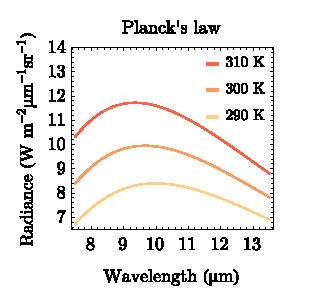
\includegraphics[scale=1]{pics/Chapter_01/PlancksLaw.eps}
		\vspace{-0.1cm}
		\caption{Radiation of black body described by Planck's law}
		\label{fig:BBradiation}
	\end{subfigure}
	\hspace{1em}
	\begin{subfigure}[t]{.3\linewidth}
		\centering
		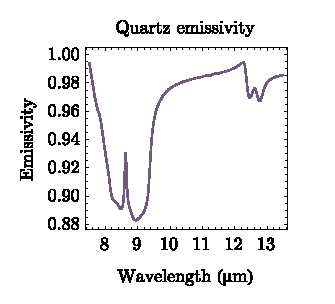
\includegraphics[scale=1]{pics/Chapter_01/QuartzSpectrum.eps}
		\vspace{-0.1cm}
		\caption{Quartz spectral emissivity}
		\label{fig:QuartzEmissivity}
	\end{subfigure}
	\hspace{1em}
	\begin{subfigure}[t]{.3\linewidth}
		\centering
		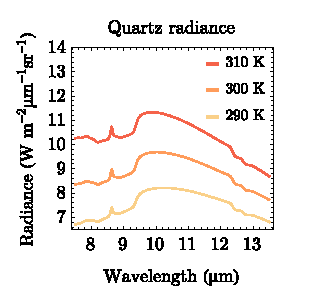
\includegraphics[scale=1]{pics/Chapter_01/QuartzRadiance.eps}
		\vspace{-0.1cm}
		\caption{Radiance of quartz}
		\label{fig:QuartzRadiance}
	\end{subfigure}
	\vspace{1.5 em}
	\caption{Principles of radiation of real surfaces.}
\end{figure}


\subsubsection*{Wien's displacement law}
The peak of black body radiation at wavelength $\lambda_{max}$ is described by Wien's displacement law \cite{H11}:
$$ \lambda_{max} = \frac{b}{T},$$
where $b$ is Wien's displacement constant ($2.8977721\times 10^{-3}\,\SI{}{m}\,\SI{}{K}$). As was mentioned before, the temperature of most of natural and artificial surfaces observed by airborne remote sensing ranges in 270 – 330 K. According to the Wien's displacement law, the peak of emitted radiation varies roughly from $8.8\,\SI{}{\micro\meter}$ to $10.7\,\SI{}{\micro\meter}$. This range is in coincidence with the atmospheric window situated between $8\,\SI{}{\micro\meter}$ to $13\,\SI{}{\micro\meter}$. The atmospheric transmittance in this atmospheric window is very high and thus it is relevant for acquisition of remotely sensed thermal data.

\subsubsection*{Kirchhoff's law of thermal radiation}
Emitting and absorbing properties of an object at local thermodynamic equilibrium surrounded by an isothermal environment are related through by Kirchhoff's law of thermal radiation \cite{K60}. It states that an object's surface absorptivity $\alpha(\lambda)$ at a given wavelength is equal to the object's surface emissivity $\varepsilon(\lambda)$ at the same wavelength:
$$ \alpha(\lambda) = \varepsilon(\lambda). $$
Energy conservation implies that energy incident to the object's surface can be reflected, transmitted or absorbed. Considering the fractions of incident energy the following equation holds:
$$ 1 = \rho(\lambda) + \tau(\lambda) + \alpha(\lambda), $$
where $\rho(\lambda)$ is the object's surface spectral reflectivity, $\tau(\lambda)$ is the object's surface spectral transmissivity and $\alpha(\lambda)$ is the object's surface spectral absorptivity. Applying Kirchhoff's law to opaque material ($\tau(\lambda) = 0$) results in following equation:
\begin{equation} 
1 = \rho(\lambda) + \varepsilon(\lambda) \quad \Rightarrow \quad \rho(\lambda) = 1 - \varepsilon(\lambda).
\label{eq:KirchHoffsLawImplication}
\end{equation}

All mentioned principles in this section will be further used in explanation of properties of airborne thermal hyperspectral data and its processing.

	\cleardoublepage
	\pagestyle{mystyle}
\chapter{Airborne thermal hyperspectral data properties}
\label{chap:Data}

This chapter provides insights into technical parameters of the TASI and processing chain of image data acquired by this sensor. Knowledge of the instrument parameters and processing chain gives important overview of the image data properties and their components. The result of the processing chain described in this chapter is a georeferenced image data containing land-leaving radiance. Such an image data form an input for further processing. Let us note that this chapter omits naming physical quantities dependent on wavelength as ``spectral'' for the sake of clarity. However, all quantities remain wavelength dependent.

\section{Instrument technical specifications}

The TASI sensor is developed by Itres Ltd. (Calgary, Canada) and is one of the very few commercially available pushbroom hyperspectral TIR sensors equipped with a mercury cadmium telluride array. Each of its 600 across-track imaging pixels contains 32 bands all of which are in the TIR region. Bands are situated in the 8 to $\SI{11.5}{\micro\meter}$ region and have a Full Width at Half Maximum $\mathrm{FWHM} \approx \SI{0.11}{\micro\meter}$ with Noise Equivalent Temperature difference $\mathrm{NE\Delta T} \approx 0.1\,\mathrm{K}$. The response functions of the TASI sensor are described by the Gaussian functions as depicted in Figure \ref{fig:ResponseFunctionsChap2}. 

The shape of the response functions implies that any quantity observed by TASI sensor is of finite spectral-bandwidth. Quantities need to be transformed to band-effective quantities in order to relate them with certain wavelengths. The band-effective quantities are obtained by using the weighted average:
%Thus quantities measured by sensor are transformed to band-effective quantities using weighted average:
\begin{equation}
	X_i = \frac{\int_{\lambda_1}^{\lambda_2} r_i(\lambda) X(\lambda) \,\mathrm{d}\lambda}{\int_{\lambda_1}^{\lambda_2} r_i(\lambda)\,\mathrm{d}\lambda},
	\label{eq:weightedAverage}
\end{equation}
where $r_i(\lambda)$ is the response function of band $i$, $\lambda_1$ and $\lambda_2$ are the lower and upper boundaries of band $i$ and $X$ can be substituted by any quantity. Figure \ref{fig:QuartzByTASIChap2} illustrate the radiance of quartz (solid line) and band-effective values of radiance measured by the TASI sensor (red dots). A sensor of this type is available at the Global Change Research Institute CAS (Brno, Czech Republic) and it is a part of the Flying Laboratory of Imaging Systems (FLIS) \cite{HF14}.

\begin{figure}[thb]
	\centering
	\vspace{1em}
	\begin{subfigure}[t]{.5\linewidth}
		\centering
		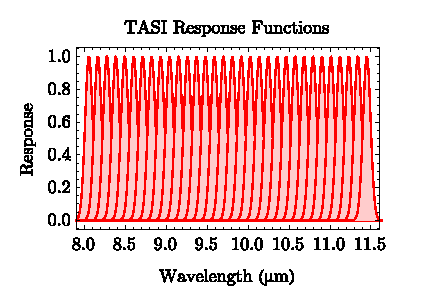
\includegraphics[scale=1]{pics/Chapter_02/TASIResponseFunctions.eps}
		\caption{Response functions of TASI sensor}
		\label{fig:ResponseFunctionsChap2}
	\end{subfigure}
	\hspace{2em}
	\begin{subfigure}[t]{.4\linewidth}
		\centering
		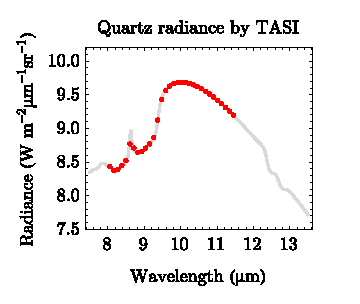
\includegraphics[scale=1]{pics/Chapter_02/QuartzByTASI.eps}
		\caption{Radiance of quartz at 300 K measured by TASI sensor}		
		\label{fig:QuartzByTASIChap2}
	\end{subfigure}
	\vspace{1.5 em}
	\caption{TASI response functions.}
\end{figure}

\section{Image data pre-processing}

The main objective of image data pre-processing is transformation of acquired raw image data into georeferenced radiance at surface level. It is accomplished by three major steps: radiometric calibration, atmospheric corrections and geometric pre-processing. Radiometric calibration converts digital numbers (DN) into values of radiance at sensor level. Atmospheric corrections compensates the influence of the intervening atmosphere and produces land-leaving radiance. Finally, the geometric pre-processing compensates for image data distortions caused by aircraft movement and registers the image data into a coordinate system.

Supportive field measurements of thermal radiance, surface temperature, emissivity and atmospheric parameters offers valuable data for calibration and validation purposes. Especially in cases of airborne image data for scientific purposes the high quality is strongly demanding. Thus it is necessary to perform supportive measurements in order to achieve precise results and determine the data quality.

It is important to emphasize that currently there does not exist any definitive standard pre-processing chain. This is caused mainly by a small number of sensors with various technical parameters and their different applications. Sensors usually have tailored pre-processing chains, which is the case of TASI sensor as well. Certain parts of processing chain are maintained by commercial tools. However, there are still parts of processing chain that need to be done by in-house tools. In Figure \ref{fig:ProcessingChain} is illustrated the processing chain used at the Global Change Research Institute CAS (Brno, Czech Republic) to pre-process image data acquired by TASI sensor. Individual parts of the diagram will be discussed in the following text. The radiometric calibration and atmospheric corrections are demonstrated with an example of quartz radiance at \SI{300}{\kelvin} as depicted in Figure \ref{fig:RadAtmCorOfQuartz}.

\begin{figure}[thb]
	\centering
	\vspace{0.7 em}
	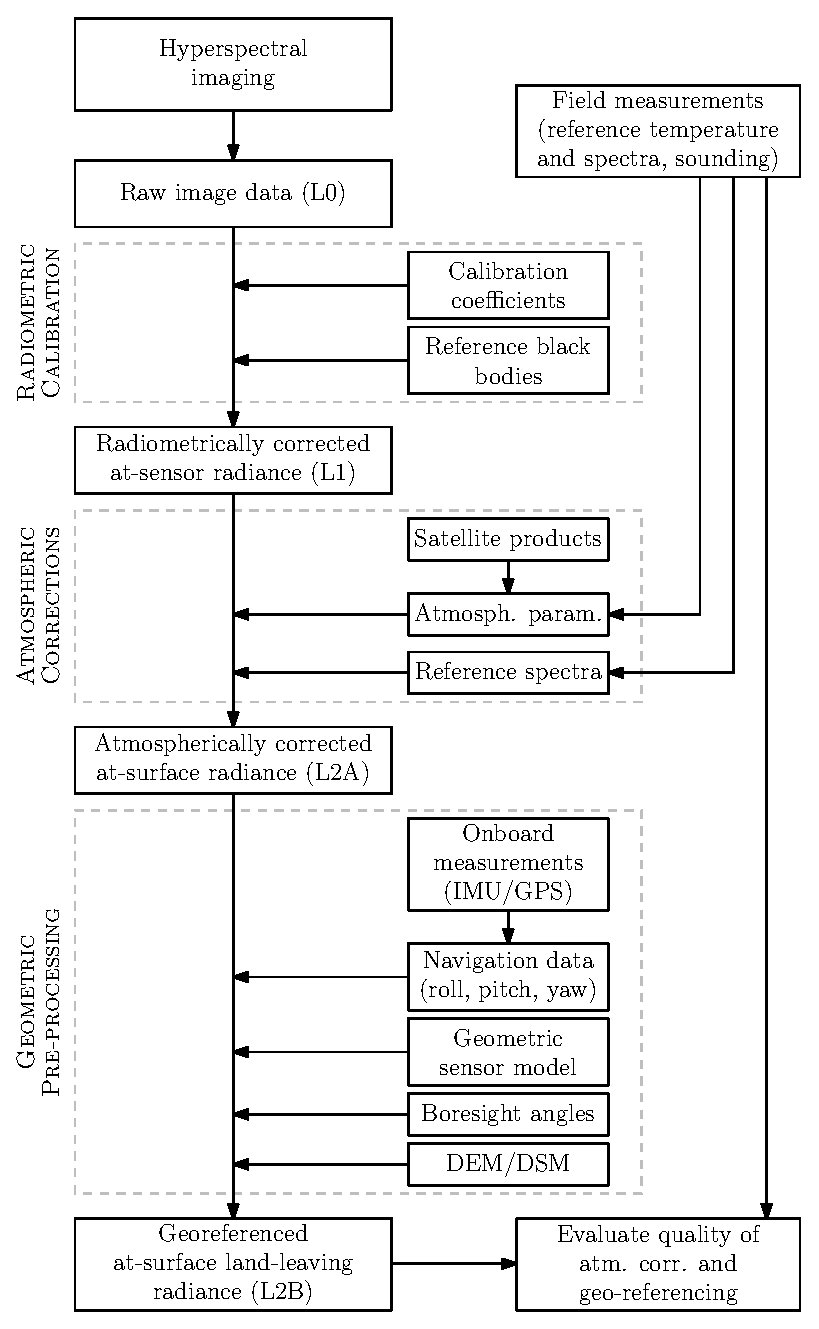
\includegraphics[scale=1]{pics/Chapter_02/Fig_2_3.eps}
	\label{fig:ProcessingChain}
	\vspace{2 em}
	\caption{Processing chain applied to image data acquired by TASI sensor.}
	\label{fig:ProcessingChain}
	\vspace{0.7 em}
\end{figure}

\begin{figure}[htb]
	\centering
	\vspace{1em}
	\begin{subfigure}[t]{.3\linewidth}
		\centering
		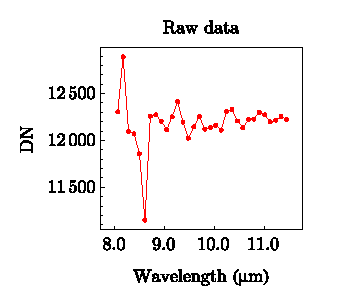
\includegraphics[scale=1]{pics/Chapter_02/calibration-1-DN.eps}
		\vspace{-0.4cm}
		%\caption{Raw image of quartz in DN values}
		\caption{}
	\end{subfigure}
	\hspace{1em}
	\begin{subfigure}[t]{.3\linewidth}
		\centering
		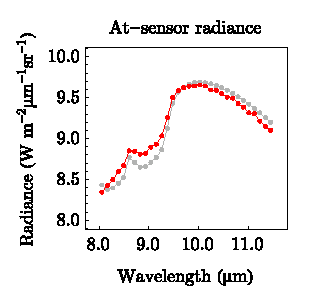
\includegraphics[scale=1]{pics/Chapter_02/calibration-2-Lm.eps}
		\vspace{-0.4cm}
		%\caption{At-sensor radiance of quartz}
		\caption{}
	\end{subfigure}
	\hspace{1em}
	\begin{subfigure}[t]{.3\linewidth}
		\centering
		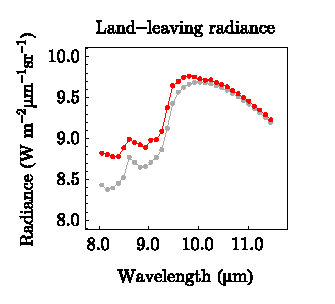
\includegraphics[scale=1]{pics/Chapter_02/calibration-3-Lll.eps}
		\vspace{-0.4cm}
		%\caption{Land-leaving radiance of quartz.}
		\caption{}
	\end{subfigure}
	\vspace{1.5 em}
	\caption{Example of data at various processing stages. Data simulates quartz at \SI{300}{\kelvin} as would be acquired by TASI sensor at altitude of \SI{2000}{\meter} under summer mid-latitude atmosphere: (a) shows raw data, (b) shows data after radiometric calibration (in red) and (c) shows data after corrections of atmospheric transmissivity and upwelling atmospheric radiance (in red). In cases (b) and (c) pure quartz radiance are shown in gray.}
	\label{fig:RadAtmCorOfQuartz}
\end{figure}

\subsection*{Radiometric calibration}

Thermal radiation incident upon the sensor array originates from many additive components (e.g. observed scene, instrument enclosure, intervening atmosphere and others). Incident thermal radiation produces an electrical signal, which is proportional to radiant intensity. This electrical signal is then amplified and converted into voltage and subsequently into DN values (as depicted in Figure \ref{fig:RadAtmCorOfQuartz}a). Radiometric calibration consists of separating signal from the viewed scene and converting it into physical units of radiance. Atmosphere influence is not accounted in this process and thus after radiometric calibration one gets radiance at sensor level (as depicted in Figure \ref{fig:RadAtmCorOfQuartz}b).

The relationship between DN and at-sensor radiance $L_\mathrm{m}$ is the following:
$$ \mathrm{DN} = a + b L_\mathrm{m}, $$
where $a$ and $b$ are calibration coefficients. The calibration coefficient $a$, also known as offset, represents radiation originating from instrument enclosure, sensor dark current and electronic offset. The calibration coefficient $b$, also called gain, determines sensor radiant sensitivity. Calibration coefficients are determined by imaging a set of reference black bodies of known temperature and emissivity. In this context, the term black body is meant to be a surface with emissivity very close to unity. These coefficients are usually determined applying one of two methods: 1) imaging two black bodies at different temperature directly before imaging, or 2) combining black body image data from laboratory and black body image data acquired before imaging.

In the first case are usually used two black bodies of different temperatures. Temperatures of these black bodies enclose temperatures expected to occur in the scene. Let us consider the radiance of cold black body $L(T_\mathrm{C})$ and the radiance of hot blackbody $L(T_\mathrm{H})$. The calibration coefficients can be obtained from:
\begin{eqnarray*}
	a &=& \frac{\mathrm{DN}_\mathrm{H} L(T_\mathrm{C}) - \mathrm{DN}_\mathrm{C} L(T_\mathrm{H}) }{ L(T_\mathrm{C}) - L(T_\mathrm{H}) } \\
	b &=& \frac{\mathrm{DN}_\mathrm{C} - \mathrm{DN}_\mathrm{H}}{ L(T_\mathrm{C}) - L(T_\mathrm{H}) },
\end{eqnarray*}
where $\mathrm{DN}_\mathrm{C}$ and $\mathrm{DN}_\mathrm{H}$ are digital numbers measured by sensor viewing cold black body and hot black body, respectively. This procedure is commonly used in case of other instruments for measuring thermal radiation, such as $\mathrm{\mu}$FTIR \cite{HK96}.

\newpage
The determination of calibration coefficients in the second case assumes that gain calibration coefficient $b$ does not change under different conditions. Thus, it is sufficient to perform series of black body measurements at different temperatures in order to determine gain calibration coefficient $b$. These measurements can be performed in the laboratory once per season. However, offset calibration coefficient $a$ does not remain stable and changes under different conditions. Hence, it is necessary to image a black body at known temperature directly before acquisition to account for variability of this coefficient.

Again, it is important to emphasize that all quantities and both calibration coefficients are wavelength dependent. Spectral calibrations are part of the radiometric calibrations. To determine spectral calibrations, band centers of every pixel using laser beam at different wavelengths are determined in the laboratory. Determined positions do not change over time significantly. However, the spectral shift occurs under different conditions and thus it needs to be determined for every scene. Spectral shift estimation is usually based on the spectral features of the atmosphere or certain materials.

In case of TASI sensor, commercial software for radiometric calibration delivered by Itres company (Calgary, Canada) is used. SparCal software \cite{software:SparCal} is used to determine all parameters necessary for radiometric calibrations from laboratory measurements. RCX software \cite{software:RCX} is used for additional  estimation of calibration parameters and for processing raw image data. The resulting radiometrically calibrated image data are radiance at sensor level $L_\mathrm{m}$.

\subsection*{Atmospheric corrections}

Radiometric calibrations deliver image data containing radiation from the surface, attenuated by atmosphere, plus radiation from the atmosphere along the line of sight. Thus the measured radiance at sensor level ($L_\mathrm{m}$) consists mainly of radiance emitted from the land surface, downwelling atmospheric radiance ($L^\downarrow_\mathrm{atm}$) reflected by the surface and the atmospheric upwelling radiance ($L^\uparrow_\mathrm{atm}$). The sum of all these components is expressed by a radiative transfer equation (RTE) as follows:
\begin{equation} 
\label{eq:RTE}
L_\mathrm{m} = \tau \varepsilon B(T_\mathrm{s}) + \tau (1 - \varepsilon) L^\downarrow_\mathrm{atm} + L^\uparrow_\mathrm{atm},
\end{equation}
where $B(T_\mathrm{s})$ is radiance of the surface at temperature $T_\mathrm{s}$ according to the Planck's law, $\varepsilon$ is the surface's emissivity and $\tau$ is atmospheric transmittance. It is important to emphasize that all elements in the equation are wavelength dependent but notation for this is omitted for the sake of clarity. Since sensors are of finite bandwidth, quantities in eq. (\ref{eq:RTE}) are replaced by band-effective equivalents according to the eq. (\ref{eq:weightedAverage}). Moreover, RTE can be used under the assumption of cloud-free atmosphere under local thermodynamic equilibrium. The meaning of the RTE is illustrated in the Figure \ref{fig:FigRTE}, where $\rho$ is reflectivity. Kirchhoff's law of thermal radiation implies that reflectivity $\rho$ can be rewritten as $(1 - \varepsilon)$ for opaque materials, as shown in eq. (\ref{eq:KirchHoffsLawImplication}).

\begin{figure}[htbp]
	\centering
	\vspace{1em}
	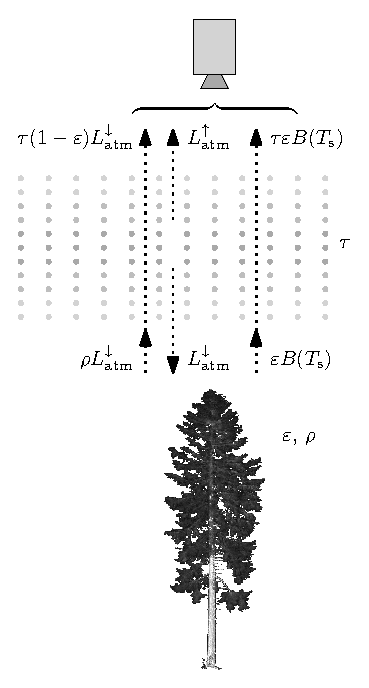
\includegraphics{pics/Chapter_02/Fig_3_2.eps}
	\vspace{1.5 em}
	\caption{The radiance incident to the sensor in the thermal region originates mainly from three sources: 1) radiance $\tau\varepsilon B(T_s)$ emitted by an object; 2) reflected downwelling atmospheric radiance $\tau(1-\varepsilon)L_\mathrm{atm}^\downarrow$; 3) upwelling atmospheric radiance $L_{atm}^\uparrow$ emitted by the atmosphere itself.}
	\label{fig:FigRTE}
\end{figure}

The goal of the atmospheric corrections is to determine atmospheric transmittance, downwelling and upwelling atmospheric radiance and compensate for them. The quantification of these quantities is usually based on radiative transfer models of the atmosphere. For this purpose MODerate resolution atmospheric TRANsmission (MODTRAN) model \cite{BG06} is usually used. MODTRAN simulates atmospheric parameters such as atmospheric transmittance, downwelling and upwelling atmospheric radiance based on input parameters such as vertical profiles of water vapour content and temperature, CO$_2$ concentration, the choice of model atmosphere (if measured profiles are not available) and many others. In general, input parameters can be obtained in two ways: 1) by \textit{in-situ} measurements; 2) by satellite-based products.

The most common \textit{in-situ} measurement is radio sounding. A radiosonde is launched during the overflight and it is used to measure vertical temperature and water vapour profile of the atmosphere. Other \textit{in-situ} instruments can be used as well, for example sunphotometer for obtaining water vapor content or different radiometers for measuring sky or surface radiance. Another source of water vapour and temperature profiles is satellite-based products acquired close to the time of aircraft overflight. The most common is MOD07\_L2 product \cite{B11} generated by Moderate Resolution Imaging Spectroradiometer (MODIS) instrument. Illustration of the transmittance, downwelling and upwelling atmospheric radiance generated by MODTRAN using MOD07\_L2 products as input are depicted in Figure \ref{fig:AtmParams}.

\begin{figure}[htb]
	\centering
	\vspace{1em}
	\begin{subfigure}[t]{.3\linewidth}
		\centering
		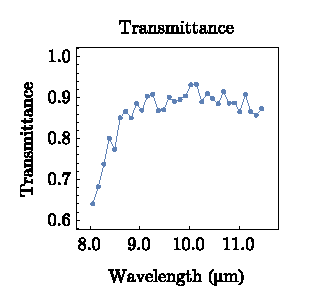
\includegraphics[scale=1]{pics/Chapter_02/Transmittance.eps}
		\vspace{-0.4cm}
		%\caption{Atmospheric transmittance}
		\caption{}
	\end{subfigure}
	\hspace{1em}
	\begin{subfigure}[t]{.3\linewidth}
		\centering
		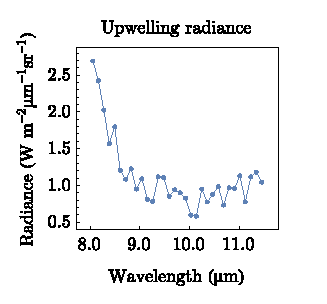
\includegraphics[scale=1]{pics/Chapter_02/Upwelling.eps}
		\vspace{-0.4cm}
		%\caption{Upwelling atmospheric radiance}
		\caption{}
	\end{subfigure}
	\hspace{1em}
	\begin{subfigure}[t]{.3\linewidth}
		\centering
		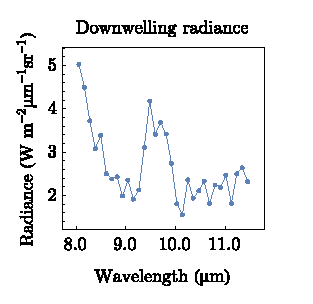
\includegraphics[scale=1]{pics/Chapter_02/Downwelling.eps}
		\vspace{-0.4cm}
		%\caption{Downwelling atmospheric radiance}
		\caption{}
	\end{subfigure}
	\vspace{1.5 em}
	\caption{Example of atmospheric parameters used for atmospheric correction of TASI image data acquired at altitude of \SI{2000}{\meter} above surface during summer season.}
	\label{fig:AtmParams}
\end{figure}

In case of thermal hyperspectral images, various algorithms for estimating atmospheric effects based just on the image data itself were developed. Usually it is applied to one of the following: In-Scene Atmospheric Corrections (ISAC) introduced by Young et al. \cite{Y02} and Autonomous Atmospheric Compensation (AAC) introduced by Gu et al. \cite{GG00}. The advantage of using one of these algorithms is that no supporting data are necessary. The drawback of these methods remains in estimation of just atmospheric transmittance and upwelling atmospheric radiance.

Once all the atmospheric parameters are determined, it remains to compensate for them. Compensating for atmospheric transmittance and upwelling atmospheric radiance leads to land-leaving radiance ($L_\mathrm{LL}$):
\begin{equation}
\label{eq:landleavingRadiance}
L_\mathrm{LL} = \varepsilon B(T_\mathrm{s}) + (1 - \varepsilon) L^\downarrow_\mathrm{atm}.
\end{equation}
The example of land-leaving radiance is shown in Figure \ref{fig:RadAtmCorOfQuartz}c. The contribution fro downwelling atmospheric radiance is not possible to separate without knowledge of emissivity. Hence, image data after atmospheric corrections are made of land-leaving radiance $L_\mathrm{LL}$. Compensation for downwelling atmospheric radiance is part of the temperature and emissivity separation described in Chapter \ref{chap:TES}.

Atmospheric corrections for the TASI sensor, as part of processing chain, are not performed by commercial products. However, there exists commercial tools that allow complex solution for atmospheric corrections. An example of such a tool is ATCOR \cite{RS02} which is based on look-up tables generated by MODTRAN and takes into account terrain topography and sensor parameters. It offers basic temperature and emissivity separation algorithms as well. Apart from the mentioned solution, atmospheric corrections rely on extracting data from \textit{in-situ} measurements or satellite products, running radiative transfer models and applying derived atmospheric parameter on image data. Alternatively, algorithms for atmospheric parameters estimation from image data can be implemented. In both cases, atmospheric corrections involve creating in-house tools.

%\begin{figure}[htb]
%	\centering
%	\vspace{1em}
%	\begin{subfigure}[t]{.3\linewidth}
%		\centering
%		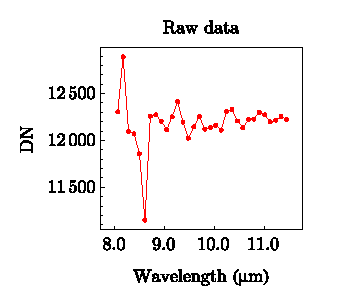
\includegraphics[scale=1]{pics/Chapter_02/calibration-1-DN.eps}
%		\vspace{-0.4cm}
%		%\caption{Raw image of quartz in DN values}
%		\caption{}
%	\end{subfigure}
%	\hspace{1em}
%	\begin{subfigure}[t]{.3\linewidth}
%		\centering
%		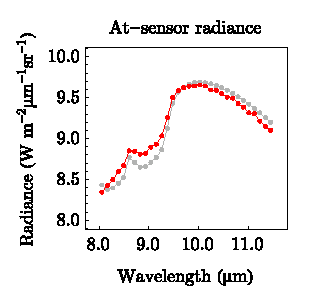
\includegraphics[scale=1]{pics/Chapter_02/calibration-2-Lm.eps}
%		\vspace{-0.4cm}
%		%\caption{At-sensor radiance of quartz}
%		\caption{}
%	\end{subfigure}
%	\hspace{1em}
%	\begin{subfigure}[t]{.3\linewidth}
%		\centering
%		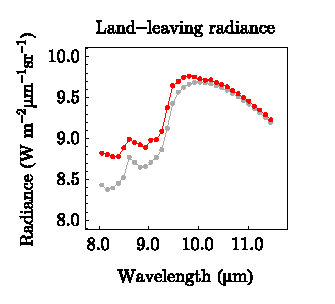
\includegraphics[scale=1]{pics/Chapter_02/calibration-3-Lll.eps}
%		\vspace{-0.4cm}
%		%\caption{Land-leaving radiance of quartz.}
%		\caption{}
%	\end{subfigure}
%	\vspace{1.5 em}
%	\caption{Example of data at various processing stages. Data simulates quartz at \SI{300}{\kelvin} as would be acquired by TASI sensor at altitude of \SI{2000}{\meter} under summer mid-latitude atmosphere: (a) shows raw data, (b) shows data after radiometric calibration (in red) and (c) shows data after corrections of atmospheric transmissivity and upwelling atmospheric radiance (in red). In cases (b) and (c) pure quartz radiance are shown in gray.}
%	\label{fig:RadAtmCorOfQuartz}
%\end{figure}

\subsection*{Geometric pre-processing}

Acquired image data are distorted during their acquisition and geometric pre-processing accounts for all factors causing these distortions. During geometric pre-processing aircraft motion, terrain variations and geometric sensor model are taken into account in order to register image data into reference frame.

Ancillary data about aircraft position and movement, terrain structure and geometric sensor model are necessary. The aircraft needs to be equipped with IMU/GNSS systems for recording aircraft position (longitude, latitude and altitude) and aircraft orientation (roll, pitch and heading angles). Terrain structure is obtained from Digital Surface Model (DSM) or Digital Elevation Model (DEM). These data are derived from aerial laser scanning or from stereo images. Aerial laser scanning can be performed either simultaneously with image data acquisition or separately. Other sources of DEM/DSM are national services or~satellite products (e.g. ASTER product AST14DEM). The geometric sensor model is usually delivered by the sensor manufacturer.

The process applied on image data during geometric pre-processing is called geo-orthoreferencing. It consists of two successive steps: direct image data geocoding and resampling. Direct image data geocoding consists of geometric corrections and orthogonalization of the image data. These are further resampled into a regular grid of the reference frame with the desired coordinate system (e.g. Universal Transverse Mercator coordinate system). Image data are resampled into desired spatial resolution applying nearest neighbor, bilinear or cubic interpolation. For scientific purposes nearest neighbor interpolation is commonly used since it preserves spectral information and does not combine spectra from surrounding pixels.

Geometric pre-processing of image data acquired by TASI sensor are performed by GeoCor software \cite{software:GCSS} delivered by Itres company (Calgary, Canada). The difference between distorted image data and georeferenced image data is illustrated in Figure \ref{fig:Georeferencing}. 

\begin{figure}[thb]
	\centering
	\vspace{1em}
	\begin{subfigure}[t]{.38\linewidth}
		\centering
		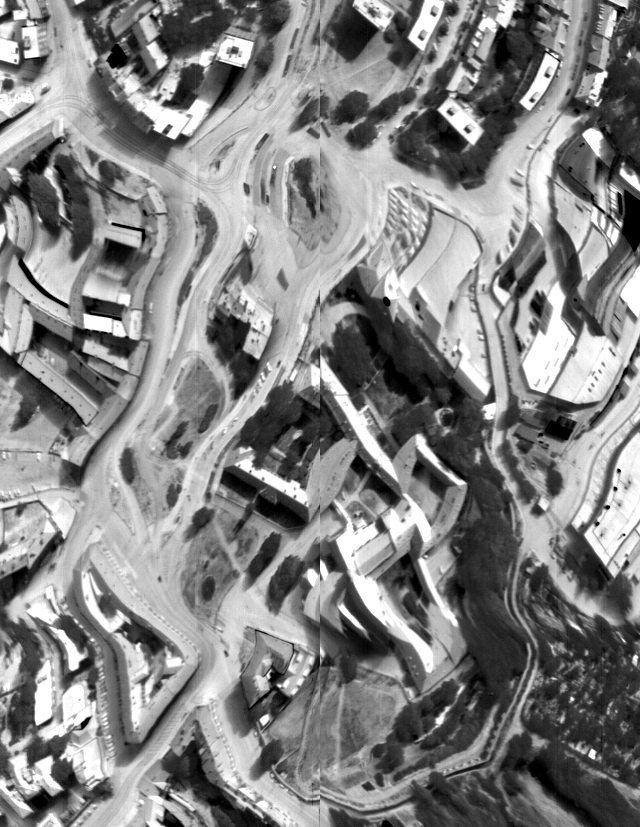
\includegraphics[scale=0.24]{pics/Chapter_02/TASIcalibrated.png}
		\caption{Distorted raw geometry image data.}
		\label{fig:ResponseFunctions}
	\end{subfigure}
	\hspace{2em}
	\begin{subfigure}[t]{.52\linewidth}
		\centering
		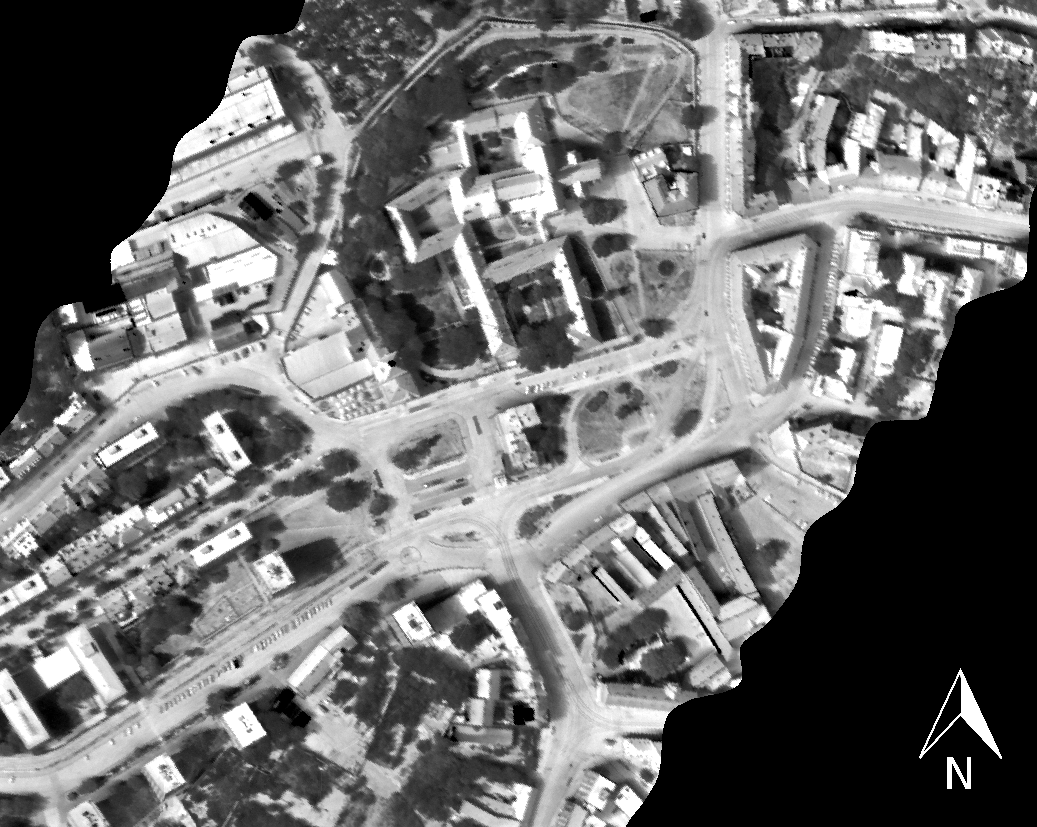
\includegraphics[scale=1]{pics/Chapter_02/TASIgeoreferencedcut.png}
		\caption{Georeferenced image data.}		
		\label{fig:QuartzByTASI}
	\end{subfigure}
	\vspace{1.5 em}
	\caption{Illustration of land-leaving radiance image data before and after geometric pre-processing.}
	\label{fig:Georeferencing}
\end{figure}




	\cleardoublepage
	\pagestyle{mystyle}
\chapter{Temperature and emissivity separation}
\label{chap:TES}

Pre-processed thermal image data provide valuable information about the properties of the observed surfaces, most importantly their temperature and~emissivity. But in~order to determine temperature and~emissivity from observed radiance one must solve a system of RTEs. Data from multispectral and~hyperspectral TIR sensors offer the opportunity to derive both the temperature as well as emissivity spectrum, which can be used to characterize the material composition of surfaces. However, observing radiance in $N$ bands yields $N$ radiative transfer equations but $N+1$ unknowns ($N$ emissivities plus temperature), which results in~the underdetermined system of equations. The estimation of temperature and~emissivity from such a system of equations is usually addressed as \textit{temperature-emissivity separation}. This chapter describes several approaches for separating temperature and emissivity. It firstly introduces a few commonly used methods and~then focuses on the most popular approach called the Temperature and~Emissivity Separation algorithm (TES). The last part of this chapter focuses on enhancing the accuracy and~precision of the products generated by the TES algorithm. The main improvement is accomplished by replacing one of the TES modules with a newly designed one that takes advantage of a relationship between brightness temperature (i.e. temperature obtained from land-leaving radiance under the assumption of emissivity $\varepsilon = 1$) and~emissivity. The improved TES algorithm is called Optimized Smoothing for Temperature Emissivity Separation (OSTES) and~is introduced in~\cite{PK16}.

\section{Available approaches}
\label{sec:AvailApproach}

Many approaches have been developed to overcome the problem of having an underdetermined system of RTEs \cite{LT13}. Methods used to overcome the problem of underdetermined system of RTEs are usually based on adding empirical or semiempricial constraints. 

Algorithms for temperature and~emissivity estimation depend on sensor architecture and~acquisition context. Some algorithms require knowledge of Normalized Difference Vegetation Index (NDVI) \cite{SR00}, surface type \cite{SW98} or even emissivity \cite{JC09}. Others are based on multitemporal \cite{W08} or multiangle \cite{SS07} acquisition. Only a few algorithms can retrieve temperature and~emissivity from a single scene without ancillary surface information, whether using multispectral or hyperspectral data. The most common are: the grey body emissivity method \cite{BP96}, the linear emissivity constraint temperature emissivity separation method \cite{WW11}, spectral smoothing \cite{B08} and~the TES algorithm \cite{GR98}. Principles of the last four mentioned methods are described in~the following text. The most attention is paid to the TES algorithm, as it is the most popular and~it is widely applied to many data.

\subsection*{Gray body emissivity method}

Barducci and~Pippi \cite{BP96} proposed an algorithm that is based on an assumption of flat spectral emissivity beyond $\SI{10}{\micro\meter}$. To solve the system of RTEs it is enough to find at least two spectral bands with the same emissivity. This can be achieved in~case of airborne thermal hyperspectral data. The drawback of this method is its sensitivity to instrument noise.

\subsection*{Linear emissivity constraint temperature emissivity separation method}

As Wang et al. \cite{WW11} describe, this method is based on the idea of substituting spectral emissivity with a piecewise linear function. The emissivity spectrum is divided into segments, in~which spectral emissivities are assumed to be linearly dependent on wavelength. Thus, it is necessary for every segment to estimate gain and~offset. It implies that the number of spectral bands has to be equal to, or greater than number of unknowns resulting from segmentation to piecewise linear functions.

\subsection*{Spectral smoothing}

The spectral smoothing algorithm, also known as ARTEMISS (Automatic Retrieval of Temperature and~EMIssivity using Spectral Smoothness), was reported by Borel at \cite{B98} and~\cite{B08}. The algorithm is based on the assumption that spectra of solids are much more smooth than spectra of gases. Thus by smoothing spectra one removes spectral features introduced by atmosphere and~obtains spectral emissivity. Moreover, current implementation described in~\cite{B08} includes modified ISAC algorithm called ARTISAC, which estimates atmospheric transmissivity for further choice of the correct atmospheric model. Atmospheric models contain so called TUD (atmospheric Transmissivity, Upwelling and~Downwelling atmospheric radiance) and~are stored in~look-up tables (LUT). Then temperature is varied until the spectral emissivity is the smoothest possible, where the smoothness criterion is the standard deviation of measured radiance minus simulated radiance. The spectral smoothness method can be described briefly by following steps:
\begin{enumerate}
	\item Estimation of atmospheric transmissivity using ARTISAC algorithm
	\item Determination of few the closest atmosphere models from TUD-LUT according to the estimated atmospheric transmissivity
	\item Use of these atmosphere models as input to spectral smoothness algorithm for a few pixels chosen from the image and~the atmosphere model, which results in~smoothest emissivity in~most of the cases, is chosen as the correct one
	\item Use chosen atmosphere model for the whole image and~estimate temperature and~emissivity by applying the spectral smoothing procedure
\end{enumerate}

\section{Temperature and~emissivity separation algorithm (TES)}
\label{sec:TES}

The TES algorithm was originally developed for the ASTER sensor \cite{GR98}. ASTER was launched in~December 1999 onboard NASA's Terra platform. TES has since then found widespread use with other multispectral and~hyperspectral sensors. Several studies have discussed the implementation of TES with AHS data \cite{SJ06, JS12}. Application of TES to data acquired by the TASI sensor is mentioned in~a few studies as well \cite{WX11, PP12}. Apart from the mentioned sensors, the TES algorithm has been modified for the Digital Airborne Imaging Spectrometer (DAIS) sensor \cite{SJ02}. Concerning spaceborne sensors, the TES algorithm has also been suggested for the Spinning Enhanced Visible and~Infrared Imager (SEVIRI) \cite{JS14}, the MODIS \cite{HH11} and~the Multispectral Thermal Imager (MTI) \cite{MB02} data processing. Moreover, the TES algorithm is being suggested for the future HyspIRI mission \cite{HH11-2}.

The TES algorithm is based on a semi-empirical relationship between spectral contrast (i.e. difference between the highest and~lowest values in~the emissivity spectrum) and~the minimum emissivity. The algorithm consists of three modules, namely the Normalization Emissivity Module (NEM) \cite{G86}, the Ratio module and~the Maximum-Minimum Difference (MMD) module \cite{M94}. The inputs to the algorithm are land-leaving radiance $L_\mathrm{LL}$ and~downwelling radiance $L^{\downarrow}_\mathrm{atm}$. Let us remind the reader that land-leaving radiance is obtained from eq. (\ref{eq:RTE}) by compensating for atmospheric transmissivity $\tau$ and~atmospheric upwelling radiance $L^{\uparrow}_\mathrm{atm}$:
\begin{equation}
\label{eq:landleavingRadiance}
L_\mathrm{LL} = \varepsilon B(T_\mathrm{s}) + (1 - \varepsilon) L^\downarrow_\mathrm{atm}.
\end{equation}

The NEM module performs an iterative process for estimating temperature and~emissivity, and~compensating for the downwelling radiance. The output of the NEM module is an initial estimation of temperature and~emissivity. Then the ratio module normalizes the emissivities obtained by the NEM module using their arithmetic mean. Thus one obtains the so called $\beta$ spectrum, which is less sensitive to sensor noise. Finally, the maximum and~minimum of the $\beta$ spectrum are found and~their difference (MMD) is used in~following semi-empirical relationship:
\begin{equation} 
\label{eq:MMD}
\varepsilon_\mathrm{min} = 0.994 - 0.687 \times \mathrm{MMD}^{0.737}. 
\end{equation}
Derivation of eq. (\ref{eq:MMD}) is explained in~following paragraph. Ratioing the $\beta$ spectrum back to an emissivity spectrum with knowledge of minimum emissivity increases the precision of the emissivity spectrum estimates. The band with the highest emissivity is then used for temperature estimation.

\begin{figure}[!t]
	\centering
	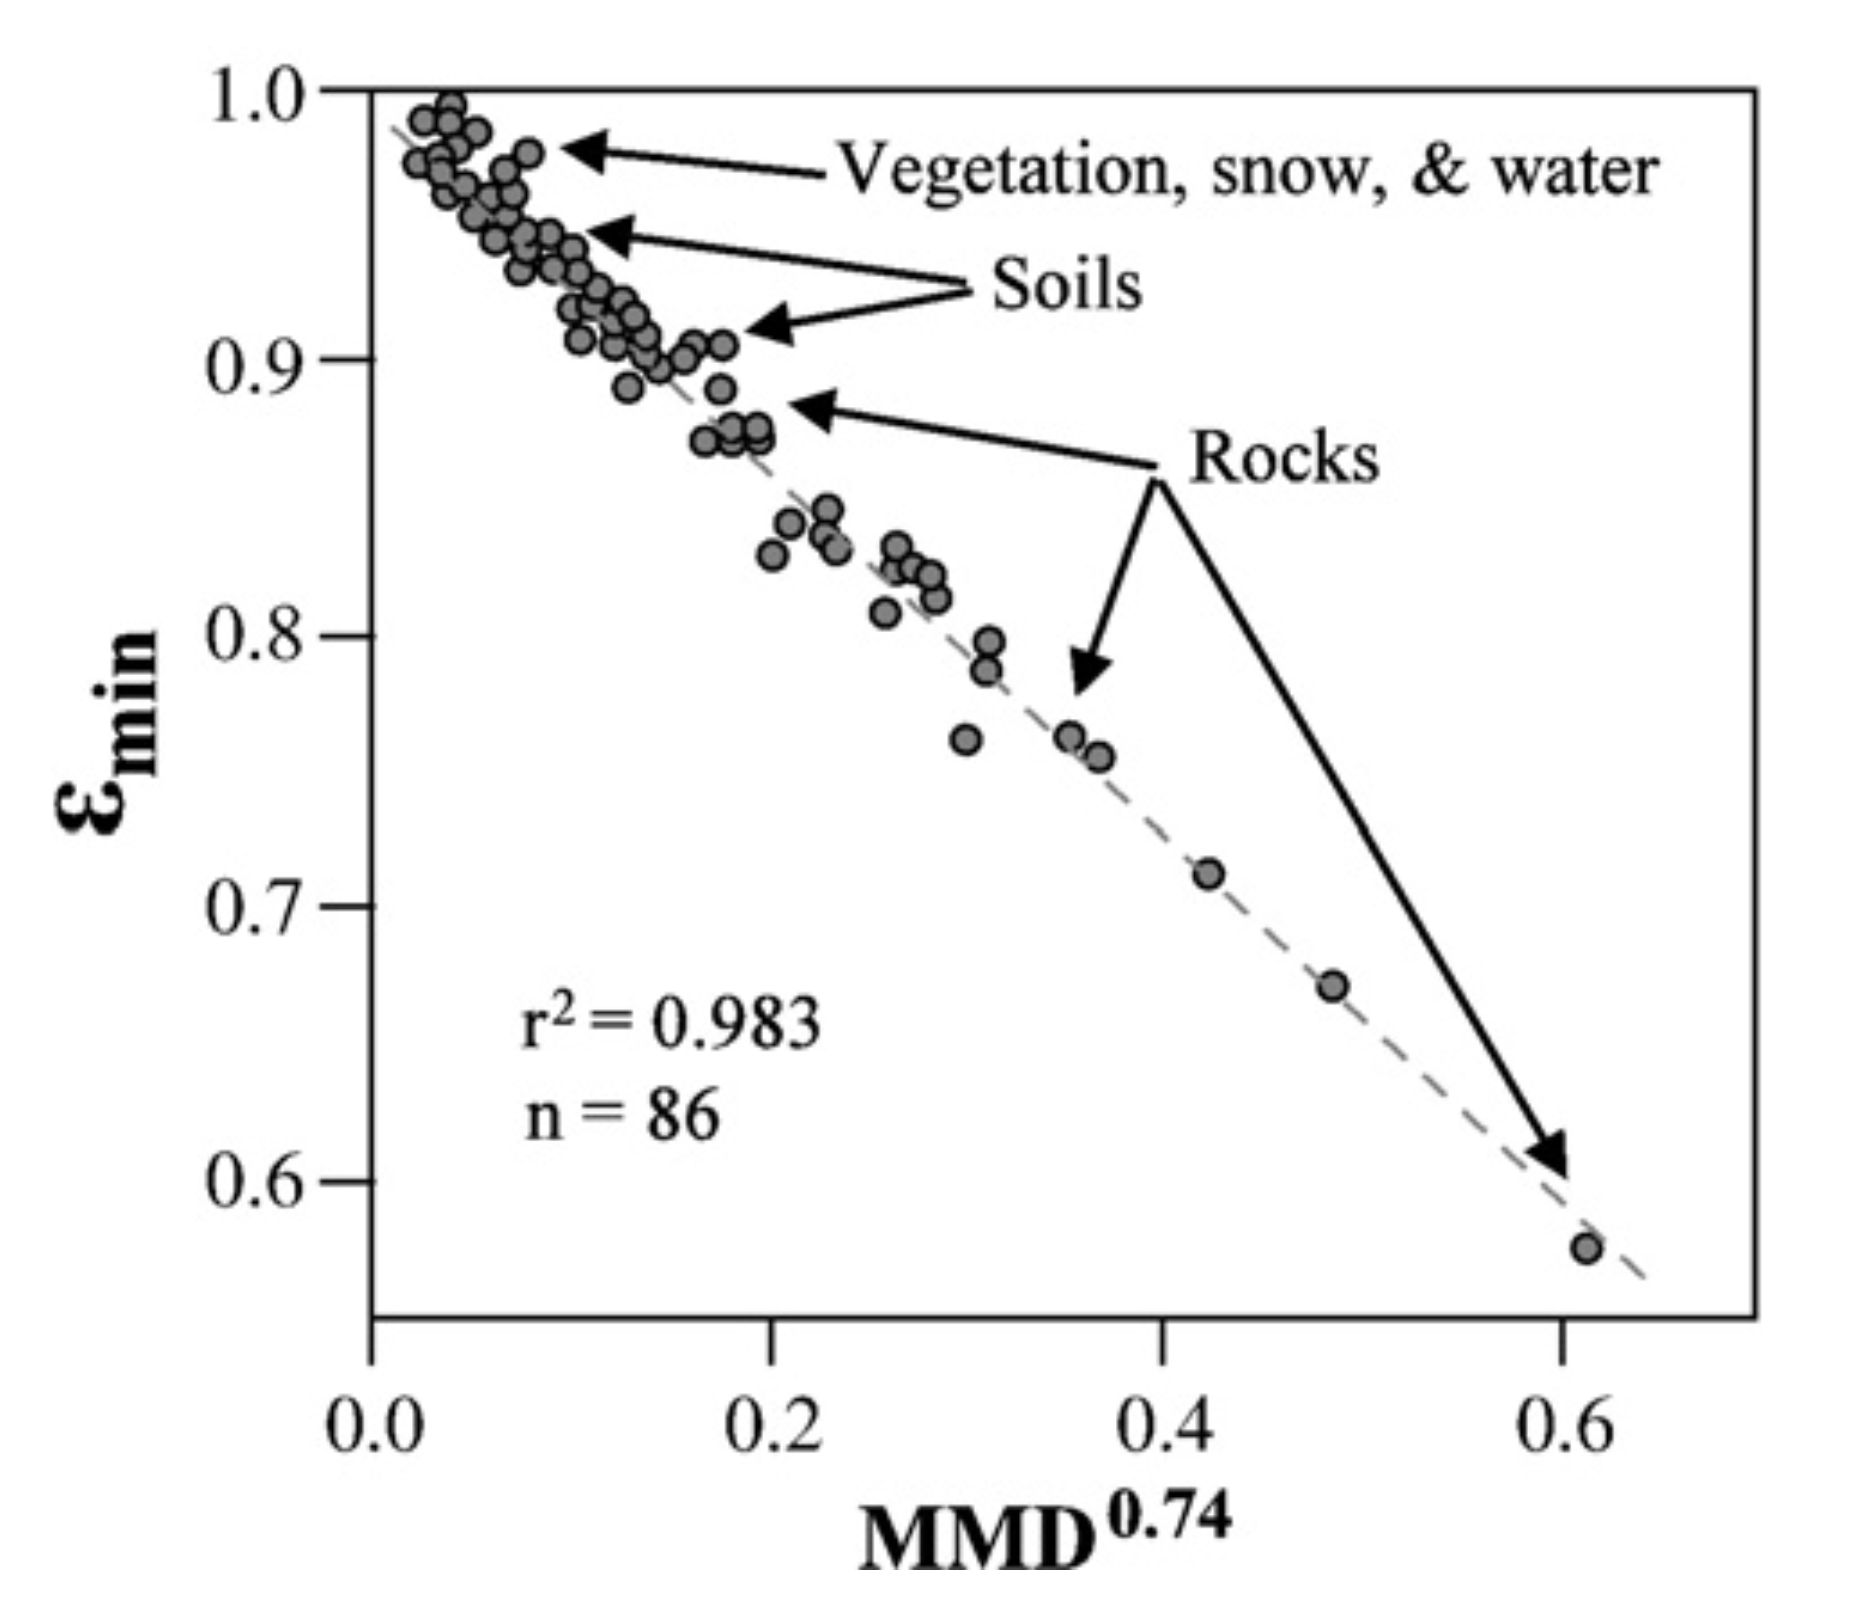
\includegraphics[scale=0.2]{pics/Chapter_03/EpsMinMMD.png}
	\vspace{1.5 em}
	\caption{Semi-empirical relationship between emissivity contrast and~minimum spectral emissivity as shown in~study reported by Sabol et al. \cite{SG09}.}
	\label{fig:EpsMinMMD}
\end{figure}

The relationship between spectral contrast and~minimum emissivity, shown in~eq. (\ref{eq:MMD}), is a regression based on 86 laboratory spectra of rocks, soils, vegetation, snow and~water chosen from the ASTER spectral library \cite{BH09}. This relationship is depicted in~the Figure \ref{fig:EpsMinMMD}. It is important to note that eq. (\ref{eq:MMD}) is tailored for the ASTER sensor. To apply  {TES to a} different sensor,  {the} regression of $\varepsilon_\mathrm{min}$ on MMD  {must be} refined by using sensor specific response functions. 

After ASTER was launched, \cite{GG06} and~\cite{SG09} suggested to replace the power regression shown in~eq. (\ref{eq:MMD}) with linear regression. The replacement is connected with modification of the threshold for separating materials with low spectral contrast. The main advantage is elimination of artefacts in~retrievals. However, the drawback is loss of accuracy in~cases of materials with low spectral contrast \cite{SG09}. The TES algorithm used for generation ASTER standard products \cite{B15}, as well as its modifications for other sensors \cite{SJ06, JS12, WX11, SJ02, JS14, HH11, MB02, HH11-2}, is based on the power law regression. Thus, in~this work the TES algorithm is considered to be that using the power regression.

\section{TES algorithm improvement}

The algorithm described below brings a new approach for separating temperature and~emissivity by replacing the NEM module in~the TES algorithm with a completely new module. The new module is based on the similarity between brightness temperature spectral features and~emissivity spectral features. Brightness temperature is obtained from land-leaving radiance under the assumption of emissivity $\varepsilon=1$ for every wavelength. Although land-leaving radiance includes some portion of reflected downwelling radiance, it still retains the spectral features arising from the emissivity of the surface materials, which is $0.6$ or higher for natural materials \cite{GR98}. Since the magnitude of downwelling radiance is usually much lower than the surface radiance the features contained in~the brightness temperature spectra may be distorted but will not be completely hidden. The new module approximates this relation between brightness temperature $T_\mathrm{b}$ and~emissivity.

\begin{figure}[!t]
	\centering
	\vspace{1em}
	\begin{subfigure}[t]{.3\linewidth}
		\centering
		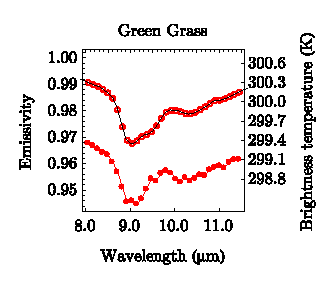
\includegraphics[scale=1]{pics/Chapter_03/GreenGrass_Emiss_vs_BrightTemp.eps}
		\caption{}
	\end{subfigure}
	\hspace{1em}
	\begin{subfigure}[t]{.3\linewidth}
		\centering
		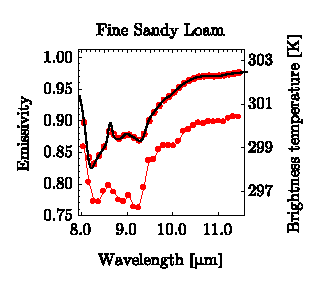
\includegraphics[scale=1]{pics/Chapter_03/FineSandyLoam_Emiss_vs_BrightTemp.eps}
		\caption{}
	\end{subfigure}
	\hspace{1em}
	\begin{subfigure}[t]{.3\linewidth}
		\centering
		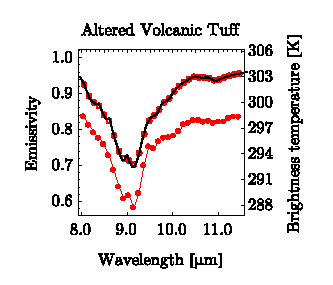
\includegraphics[scale=1]{pics/Chapter_03/AlteredVolcanicTuff_Emiss_vs_BrightTemp.eps}
		\caption{}
	\end{subfigure}
	\vspace{1.5 em}
	\caption{Emissivity spectra (black solid line) of three samples chosen from ASTER spectral library \cite{BH09}. Symbols represent band-effective values of emissivity (empty symbols) and~brightness temperature (full symbols) for TASI sensor. }
	\label{fig:emissivitySpectra_spectra}
\end{figure}

In order to demonstrate the relationship, three emissivity samples with different spectral contrasts were chosen from the ASTER spectral library \cite{BH09}, namely green grass, fine sandy loam and~altered volcanic tuff. These emissivities are depicted in~Figure \ref{fig:emissivitySpectra_spectra} (solid lines) together with corresponding band-effective values for TASI sensor (empty symbols). These emissivities were applied to Plank's law at temperature $300\,\mathrm{K}$ and~combined with downwelling radiance from standard mid-latitude summer atmosphere generated by MODTRAN \cite{BG06}. The resulting radiances, were transformed to band-effective quantities with respect to TASI response functions. Brightness temperatures for every band of each sensor were obtained by applying inverse Planck's law on a sample of land-leaving radiances under the assumption of $\varepsilon=1$. Figure \ref{fig:emissivitySpectra_spectra} also includes brightness temperatures (full symbols) in~order to demonstrate spectral similarity with emissivity. Figure \ref{fig:relationship} plots emissivity against brightness temperature for the chosen samples (empty symbols). These quantities clearly exhibit relationship with linear trend regardless of spectral contrast. Also displayed in~Figure \ref{fig:relationship} are lines that approximate this relationship, derived in~the manner described later in~the next. 

The only factor that can jeopardize the linear relationship between brightness temperature and~emissivity is the high magnitude of downwelling radiance in~comparison with surface radiance. This will occur rarely, if at all, as described in~the first paragraph of this section. Let us emphasise that the brightness temperature and~emissivity relationship can be approximated by the linear relationship at any surface temperature since we are interested in~the brightness temperature features rather than in~absolute values. The algorithm description below uses band-effective values of quantities linked to $i$-th band by subscript index $i$. 

The dependence of emissivity $ {\varepsilon_i}$ on brightness temperature $ {T_{\mathrm{b}_i}}$ will be approximated by following equation:
\begin{equation} \varepsilon_{ {i}} =  {p} T_{\mathrm{b}_{ {i}}} +  {q}, \label{eq:relationship}\end{equation}
where $ {p}$ and~$ {q}$ are empirical coefficients. These coefficients are determined by solving the system of two equations using two points, namely maximum brightness temperature coupled with emissivity equal to 1 and~minimum brightness temperature coupled with lowest emissivity $\varepsilon_\mathrm{min}$:
\begin{equation}
\begin{aligned}
	1 &=  {p} \max (T_{\mathrm{b}_{ {i}}}) +  {q}, \\
	\varepsilon_\mathrm{min} &=  {p} \min (T_{\mathrm{b}_{ {i}}}) +  {q}.
\end{aligned}
\label{eq:sytemofeq}
\end{equation}
The next step is estimation of the the lowest emissivity $\varepsilon_\mathrm{min}$.

This is done by varying $\varepsilon_\mathrm{min}$ over the range  {of possible emissivities for natural materials $[0.6,1{ {]}}$}, determining corresponding coefficients $ {p}$ and~$ {q}$ by solving eq. (\ref{eq:sytemofeq}) and~then approximating emissivity by eq. (\ref{eq:relationship}) using brightness temperature for all spectral bands. The estimated emissivity is then used together with land-leaving radiance $L_\mathrm{LL}$ and~downwelling radiance $L^\downarrow$ (subscript $_\mathrm{ATM}$ is omitted for clarity reasons) in~a computation that yields spectral radiance:
\begin{equation}
	L^{\prime}_{ {i}} = \frac{L_{\mathrm{LL}_{ {i}}}-(1-\varepsilon_{ {i}})L^\downarrow_{ {i}}}{\varepsilon_{ {i}}}.
	\label{eq:lprime}
\end{equation}
The temperature in~every spectral band is derived from spectral radiance $L^{\prime}$ applying inverse Plank's law. The highest one is chosen as the reference temperature $T_\mathrm{max}$. Finally, the estimated spectral radiance $L^{\prime}$ and~Planck's law at the reference temperature $T_\mathrm{max}$ are normalized and~compared against each other as follows:
\begin{equation*}
	\sum_{ {i}} \left| \frac{B_{ {i}}(T_\mathrm{max})}{||B(T_\mathrm{max})||_1} - \frac{L^\prime_{ {i}}}{||L^\prime||_1} \right|.
\end{equation*}
The value of $\varepsilon_\mathrm{min}$ is considered final if its corresponding spectral radiance $L^{\prime}$  {is the best fit to Plank's law}.

\begin{figure}[!t]
	\centering
	\vspace{1em}
	\begin{subfigure}[t]{.3\linewidth}
		\centering
		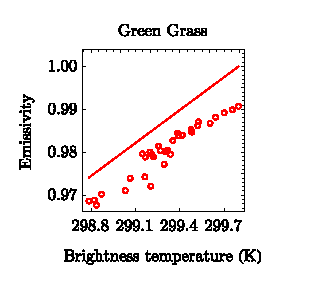
\includegraphics[scale=1]{pics/Chapter_03/GreenGrass_Emiss2BrightTemp.eps}
		\caption{}
	\end{subfigure}
	\hspace{1em}
	\begin{subfigure}[t]{.3\linewidth}
		\centering
		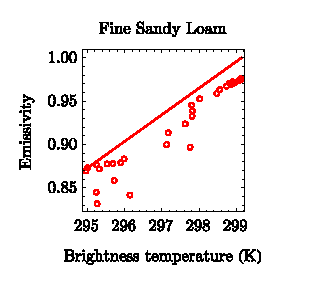
\includegraphics[scale=1]{pics/Chapter_03/FineSandyLoam_Emiss2BrightTemp.eps}
		\caption{}
	\end{subfigure}
	\hspace{1em}
	\begin{subfigure}[t]{.3\linewidth}
		\centering
		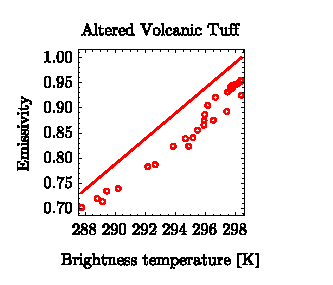
\includegraphics[scale=1]{pics/Chapter_03/AlteredVolcanicTuff_Emiss2BrightTemp.eps}
		\caption{}
	\end{subfigure}
	\vspace{1.5 em}
	\caption{Symbols represent examples of the relationship between brightness temperature $T_\mathrm{b}$ and~emissivity as would be observed by the TASI sensor. Lines illustrate the approximations of the relationship between brightness temperature and~emissivity. The procedure used for estimation of the brightness temperature and~emissivity relationship is described in~the text.}
\label{fig:relationship}
\end{figure}

The whole process of determining $\varepsilon_\mathrm{min}$ can be understood as smoothing the spectrum by finding the optimal value of $\varepsilon_\mathrm{min}$. Pseudocode depicted in~Figure \ref{fig:FunctionCode} summarizes the above described procedure as a function \textsc{SmoothingErr}($\varepsilon_\mathrm{min},L_\mathrm{LL},L^\downarrow$) evaluating the error between Planck's law and~estimated spectral radiance. This function is minimized with respect to the variable $\varepsilon_\mathrm{min}$ as follows:
\begin{equation*}
\underset{\varepsilon_\mathrm{min} \in  {[0.6,1]}}{\text{arg\,min}}\:\text{\textsc{SmoothingErr}}(\varepsilon_\mathrm{min},L_\mathrm{LL},L^\downarrow).
\label{eq:costFunction}
\end{equation*}

Continuous curves in~Figure \ref{fig:relationship} show the optimal brightness temperature and~emissivity relationship approximation. Let us emphasize that by applying emissivities obtained from the approximated relationship between brightness temperature and~emissivity to eq. (\ref{eq:lprime}), one gets $L^\prime$ as the best fit to Planck's law. This means that $B^{-1}(L^\prime_i)$ produces a temperature value for each band. These temperatures have minimum variability since they are derived from the best fit to Planck's law. Let us also remind the reader that maximum brightness temperature is coupled with emissivity equal to 1, which implies that it is a part of the set of temperatures with smallest variability. It is important to note that maximum brightness temperature $T_\mathrm{b}$ computed from land-leaving radiance is usually smaller than surface temperature $T$ computed from surface radiance. Land-leaving radiance is smaller than surface radiance since natural materials are of emissivity higher than $0.6$ and~the contribution from reflected downwelling radiance is usually much lower than surface radiance. By reason of maximum brightness temperature $T_\mathrm{b}$ being smaller than surface temperature $T$ and~by being part of the set of temperatures with smallest variability, it can be concluded that maximum temperature from the set of temperatures tends to be the closest to the surface temperature $T$ and~is therefore taken as the reference one.

\begin{figure}[!t]
\centering
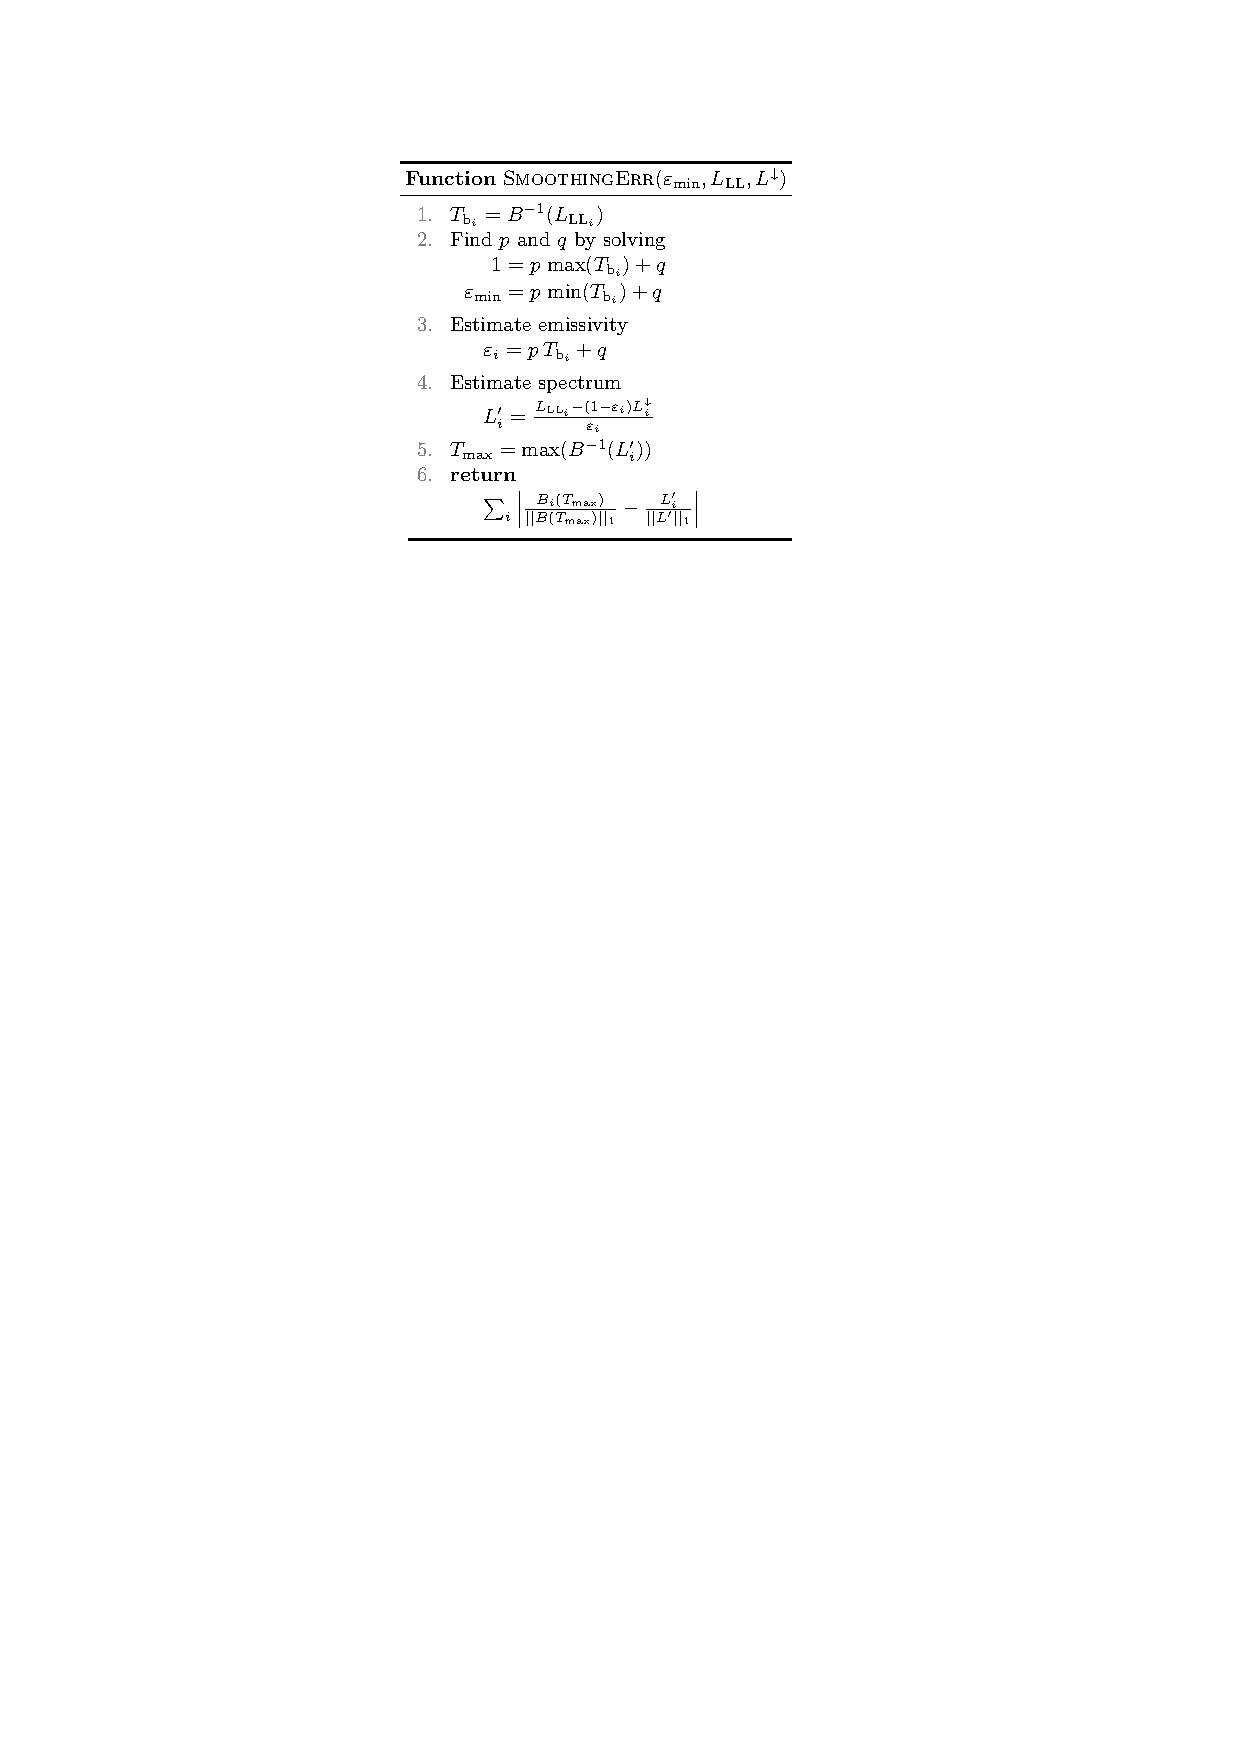
\includegraphics[scale=1]{pics/Chapter_03/pseudo_code.pdf}
\vspace{1.5 em}
\caption{Pseudocode of the function that is being minimized in~order to estimate the value of $\varepsilon_\mathrm{min}$.}
\label{fig:FunctionCode}
\end{figure}

Before passing emissivity to the Ratio and~MMD modules, it is  {recomputed} according to the following equation:
\begin{equation}
\varepsilon_{ {i}} = \frac{L_{\mathrm{LL}_{ {i}}} - L^\downarrow_{ {i}}}{B_{ {i}}(T) - L^\downarrow_{ {i}}},
\label{eq:emissivityComputation}
\end{equation}
where $T$ is the maximum temperature associated with optimal $\varepsilon_\mathrm{min}$. Equation (\ref{eq:emissivityComputation}) is derived from eq. (\ref{eq:landleavingRadiance}) and~it is important for relating temperature and~emissivity. This recomputation keeps temperature and~emissivity consistent with each other (i.e. the same temperature can be derived from any emissivity band). The emissivity is then further processed with the Ratio and~MMD modules, with minor changes to  {the} original version of the TES algorithm as it is described in~\cite{GR99} and~\cite{GR98}. These changes include: 1) there is no refinement of $\varepsilon_\mathrm{max}$ according to the emissivity spectral contrast, 2) the threshold $T_1$ for separation emissivities with small spectral contrast is not applied, and~3) the number of MMD iterations is set to one. Let us emphasize that before reporting algorithm outputs, emissivity is recomputed by eq. (\ref{eq:emissivityComputation}) using the final value of temperature.

	\cleardoublepage
	\pagestyle{mystyle}
\chapter{OSTES Validation}
\label{chap:OSTESValid}

The OSTES algorithm was tested on both synthetic and real data. Synthetic data were generated from spectral and climatological  libraries such that they cover many possible scenes and conditions. These data were simulated as would be acquired with ASTER, AHS and TASI sensor. The OSTES was further tested on a real data. For this purpose were chosen image data acquired by ASTER and TASI sensor. The ASTER image data include water bodies of the Caspian Sea and Lake Baikal. The TASI image data contain urban areas of city of Brno. 

\section{Synthetic Data}

\subsection*{Imaging Systems}

Synthetic data are intended to cover many possible situations of acquiring thermal data. Therefore three different sensor architectures were chosen to test the OSTES algorithm and compare the results with the TES algorithm.

From the wide range of airborne sensors operating in the TIR region two are chosen as examples: AHS operated by Spanish Institute of Aeronauics (INTA) and developed by ArgonST (Fairfax, USA), and TASI sensor. These sensors offer data of great importance in applications. Notable studies include areas of
mineral mapping \cite{NK14}, 
soil moisture estimation \cite{SF12}, 
urban studies \cite{SO12},
soil organic carbon estimation \cite{PC14} and
crop water stress characterization \cite{PP12},
among others.

\begin{figure}[!t]
\centering
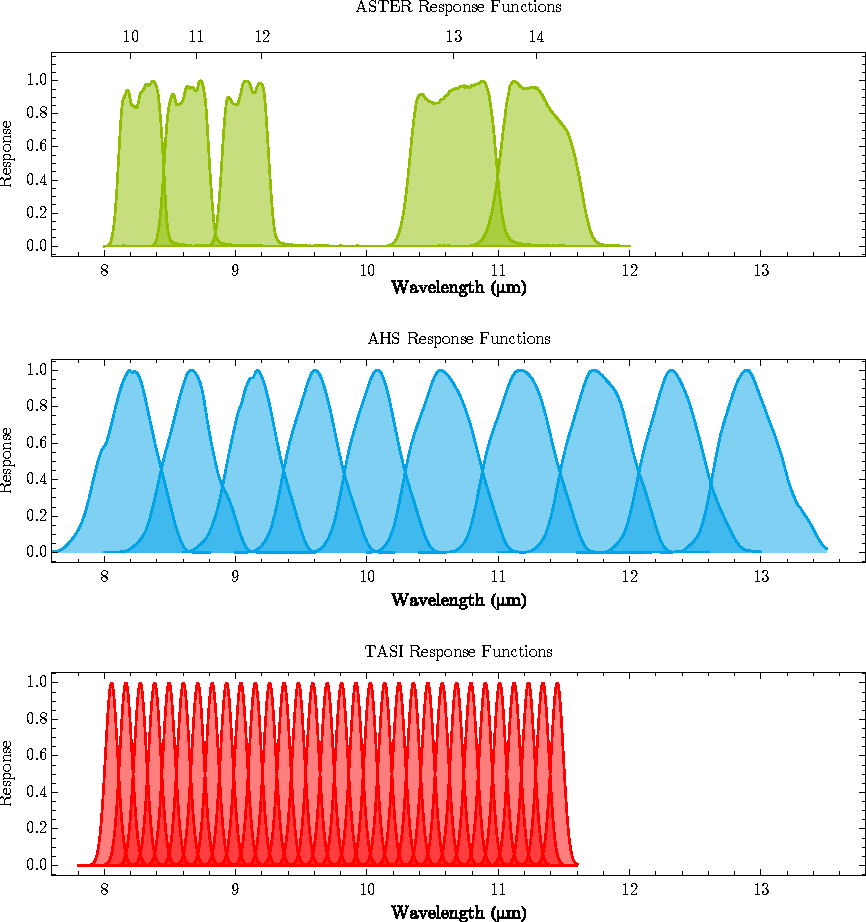
\includegraphics[width=0.9\linewidth]{pics/Chapter_04/response_functions_all.pdf}
\vspace{1.5 em}
\caption{Response functions for ASTER, AHS and TASI sensors. The ASTER Band Numbers are shown above the ASTER response functions.}
\label{fig:ResponseFunctions}
\end{figure}
 
The above-mentioned airborne sensors were chosen together with the ASTER sensor to analyze the performance of the OSTES algorithm. ASTER consists of 15 bands of which 5 are situated in TIR region with Noise Equivalent Temperature difference $\mathrm{(NE\Delta T)} \approx 0.3\,\mathrm{K}$. The spatial resolution of the TIR bands is $90\,\mathrm{m}$. The AHS sensor has been fully operational from 2005 \cite{FM05}. Its sensor operates in 80 spectral bands where the last 10 bands cover atmospheric window from 8 to $\SI{13}{\micro\meter}$ \cite{SJ06}. The AHS TIR bands have a  {Full Width at Half Maximum} $\mathrm{(FWHM)} \approx \SI{0.5}{\micro\meter}$ with $\mathrm{NE\Delta T} \approx 0.5\,\mathrm{K}$. The third sensor we will consider is TASI sensor. It contains 32 bands all of which are in the TIR region. Bands are situated in the 8 to $\SI{11.5}{\micro\meter}$ region and have a $\mathrm{FWHM} \approx \SI{0.11}{\micro\meter}$ with $\mathrm{NE\Delta T} \approx 0.1\,\mathrm{K}$. The response functions of these sensors are depicted in Figure \ref{fig:ResponseFunctions}.

\subsection*{Data Set}

A data set of 6588 samples was artificially created to compare the performance of the TES and OSTES algorithms. Samples include 108 different natural surfaces chosen from ASTER spectral library \cite{BH09} at different temperatures coupled with 61 different atmospheric conditions taken from TIGR (TOVS Initial Guess Retrieval) database \cite{CS85, CC98}. Sample temperatures range from \SI{244}{\kelvin} to \SI{310}{\kelvin}. In order to simulate real conditions, every sample at a certain temperature is coupled with a certain type of atmosphere. The chosen atmospheres represent a variety of possible conditions within polar, mid-latitude and tropical airmasses. These samples were processed to land-leaving and downwelling radiance, as standard TES algorithm input, and they were transformed to band-effective quantities with respect to the ASTER, AHS and TASI response functions. Samples were passed to the algorithms individually.

\begin{table}[!t]
\vspace{0.5em}
\footnotesize
\centering
\begin{tabular}{lcccc}
\toprule
Sensor & $a$ & $b$ & $c$ & $r^2$\\ \hline
ASTER & $0.994$ & $-0.687$ & $0.737$ & $0.983$ \\
AHS & $1.000$ & $-0.782$ & $0.817$ & $0.994$ \\
TASI & $1.001$ & $-0.737$ & $0.760$ & $0.997$ \\
\bottomrule
\end{tabular}
\vspace{1.5 em}
\caption{Regression coefficients of $\varepsilon_\mathrm{min} = a + b\:\mathrm{MMD}^c$ and coefficients of determination $r^2$.}
\label{table:MMDcoef}
\normalsize
\end{table}

\newpage
Simulated data for the ASTER sensor were processed with the current implementation of TES, as it is used for generation of ASTER standard products AST\_05 and AST\_08 \cite{B15}. The version of the original TES algorithm in cases of AHS and TASI sensors was implemented in a manner similar to that described in \cite{JS12}. In addition, the implementation omits the $\varepsilon_\mathrm{max}$ refinement for emissivities with low spectral contrast. The OSTES was applied to all sensors as it is described in section \ref{sec:TES}.

Let us remind the reader that the regression coefficients in the (\ref{eq:MMD}) needs to be refined for each sensor with respect to its response functions. The regression coefficients in (\ref{eq:MMD}) were recomputed for AHS and TASI sensors using their respective response functions. In both cases the regression was performed on a set of 108 spectra chosen from same categories and library as in the ASTER case. The coefficients for different sensors are shown in the Table~\ref{table:MMDcoef}.

\subsection*{Validation}

Samples were passed to the TES and OSTES algorithms and the temperature and emissivity results were compared with true values. We divide the results into two groups according to the emissivity spectral contrast. For each sensor type we determined a threshold for Maximum-Minimum emissivity Difference (MMD) in order to separate the samples with small spectral contrast such as water, vegetation, snow or samples with small particle sizes from other samples with higher spectral contrast. The threshold was determined for each sensor separately since different response functions and spectral ranges result in different MMD values for the same sample. The performance of both TES versions was determined by subtracting retrieved temperature from true temperature value. The temperature error and chosen MMD values for ASTER, AHS and TASI are shown in Figure~\ref{fig:SimualtedDataTemperatureErrorVsLowVsHighMMD}.

\begin{figure}[!b]
	\centering
	\vspace{1em}
	\begin{subfigure}[t]{.3\linewidth}
		\centering
		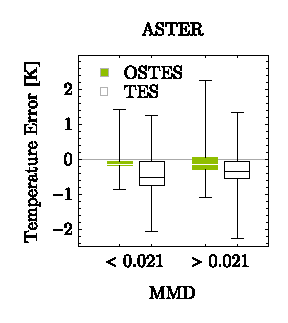
\includegraphics[scale=1]{pics/Chapter_04/Simulated_data_ASTER.eps}
		\caption{}
	\end{subfigure}
	\hspace{1em}
	\begin{subfigure}[t]{.3\linewidth}
		\centering
		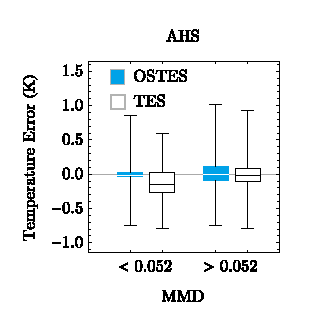
\includegraphics[scale=1]{pics/Chapter_04/Simulated_data_AHS.eps}
		\caption{}
	\end{subfigure}
	\hspace{1em}
	\begin{subfigure}[t]{.3\linewidth}
		\centering
		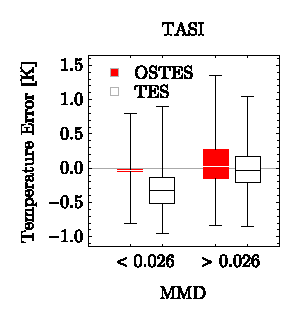
\includegraphics[scale=1]{pics/Chapter_04/Simulated_data_TASI.eps}
		\hspace{1cm}\caption{}
	\end{subfigure}
	\vspace{1.5 em}
	\caption{Box plots representing temperature error produced by OSTES and TES algorithm for ASTER, AHS and TASI sensor. Results are divided in two groups based on the Maximum-Minimum emissivity Difference (MMD) in order to demonstrate the improvement of the OSTES algorithm. Whiskers represent minimum and maximum of temperature error.}
	\label{fig:SimualtedDataTemperatureErrorVsLowVsHighMMD}
\end{figure}

Note that the temperature retrievals using OSTES are both more accurate and more precise than TES in the case of samples with low spectral contrast. It is also important to note that no significant improvement is evident for samples with higher spectral contrast. 

Let us remind the reader that every sample is processed under several different atmospheric conditions coupled with different sample temperatures. Thus the standard deviation of temperature and emissivity error is indicative of the algorithm's sensitivity to seasonal fluctuations. A comparison of standard deviations of temperature errors introduced by both TES approaches reveals that the OSTES is less sensitive to changes in atmosphere and sample temperature for samples with low MMD. However, the standard deviations of temperature errors of samples with higher MMD are similar. Standard deviations of temperature errors obtained by the OSTES and TES algorithms are summarized in the Table \ref{table:StandardDeviations}.

\section{Comparison with ASTER standard products}

The OSTES temperature and emissivity were compared with ASTER standard products AST\_08 (kinetic temperature) and AST\_05 (surface emissivity). For this purpose were chosen scenes containing water bodies. Water emissivity is well-known and does not vary significantly which offers a unique opportunity for testing various algorithm features. Water bodies are commonly used for calibration \cite{TP05-2,T05} and validation \cite{TP05, TP01} purposes.

\begin{table}[!t]
\vspace{0.5em}
\footnotesize
\centering
\begin{tabular}{cccc}
\toprule
Sensor & MMD & OSTES & TES \\ \hline
ASTER 	& $< 0.021$ & 0.25 & 0.50 \\
 		& $> 0.021$ & 0.36 & 0.43 \\ \hline
AHS 		& $< 0.052$ & 0.13 & 0.20 \\
 		& $> 0.052$ & 0.20 & 0.19 \\ \hline
TASI 	& $< 0.026$ & 0.16 & 0.32 \\
 		& $> 0.026$ & 0.32 & 0.30 \\
\bottomrule
\end{tabular}
\vspace{1.5 em}
\caption{Standard deviations of temperature errors obtained by applying OSTES and TES algorithm on simulated data as seen by ASTER, AHS and TASI grouped according to the sample Maximum-Minimum emissivity Difference (MMD). }
\label{table:StandardDeviations}
\normalsize
\end{table}

Testing was focused on: 1) investigating the impact of  various atmospheric conditions on emissivity retrievals of the same material, and 2) emissivity smoothness over homogeneous areas. Both tests were performed on ASTER scenes containing large water bodies, since water emissivity is well-known. For the first test we chose five scenes of the Caspian Sea acquired in various seasons of the year. For the second test we chose Lake Baikal. The list of all scenes used, together with their acquisition and processing dates, is given in Table \ref{table:ASTERScenes}. For every scene we downloaded ASTER standard products AST\_09T, AST\_08 and AST\_05 delivering land-leaving and downwelling radianace, surface kinetic temperature and surface emissivity, respectively. Product AST\_09T was used as input to the OSTES algorithm. The resulting temperatures and emissivities were then compared with the AST\_08 and AST\_05 standard products. The emissivity variability over large and homogeneous water bodies was chosen to be the quality indicator, since we are interested in the retrieval of material properties, which should be essentially constant over time and space.

\begin{table}[!t]
\vspace{0.5em}
\footnotesize
\centering
\begin{tabular}{cccc}
\toprule Location & Acq date (UTC) & Processing date & \parbox[c][1.4cm][c]{1.8cm}{\centering { Precipitable \\ water \\ $\mathrm{[kg\,m^{-3}]}$}} \\ \hline
Caspian Sea & 11.02.2001 - 07:35:55 & 19.11.2015 &  { 9} \\
Caspian Sea & 29.06.2002 - 07:31:47 & 19.11.2015 &  {30} \\
Caspian Sea & 21.08.2004 - 07:29:35 & 19.11.2015 &  {21} \\
Caspian Sea & 30.09.2001 - 07:35:57 & 19.11.2015 &  {28} \\
Caspian Sea & 13.11.2008 - 07:24:21 & 19.11.2015 &  {10} \\
Lake Baikal & 22.07.2002 - 04:17:29 & 27.08.2015 &  {18} \\

\bottomrule
\end{tabular}
\vspace{1.5 em}
\caption{ASTER scenes used for algorithm testing}
\label{table:ASTERScenes}
\normalsize
\end{table}

\subsection*{Caspian Sea}

From the Caspian Sea scenes we chose samples of size $40 \times 40$ pixels over uniform, cloudless waterbody. These subsets were processed by the OSTES algorithm and the emissivity results were averaged for every scene. The results are plotted in Figure \ref{fig:CaspianSeaEmissivity} along with the emissivities that were delivered in the AST\_05 product and averaged over the same spatial subset. In most cases the AST\_05 emissivity spectra appear to be closer to the sea water emissivity spectra taken from ASTER spectral library \cite{BH09}. However, the temperature retrievals of extracted samples obtained by OSTES and TES are very close (not shown). The average temperature difference of AST\_08 and OSTES results computed from all Caspian Sea samples is 0.2\,K (s.d. 0.2\,K). The fact that the temperatures obtained with the two algorithms are very close, but the emissivities are not implies that the emissivity spectra from AST\_05 product are not consistent with temperature from AST\_08 product. We verified this inconsistency by taking the temperatures delivered in AST\_08 and the downwellig and land-leaving radiances delivered in AST\_09T and putting these into (\ref{eq:emissivityComputation}) to obtain emissivities that are different from what is in the AST\_05 product. These emissivity spectra derived from AST\_08 and AST\_09T, which we refer to as ``recomputed emissivities'', are depicted on Figure \ref{fig:CaspianSeaEmissivity} as well. 

Comparison of recomputed emissivity spectra with OSTES emissivity retrievals shows that spectra are nearly identical in scenes acquired on 29.6.2002 and 30.9.2001. Agreement between these emissivity spectra are the consequence of similar AST\_08 and OSTES temperatures; the average difference is \SI{-0.04}{\kelvin} (s.d. \SI{0.15}{\kelvin}). It may be important to note that these scenes contain clouds in part adjacent to the processed sample. On the other hand OSTES results perform slightly better in scenes acquired on 11.2.2001, 21.8.2004 and 13.11.2008. The average temperature difference between AST\_08 and OSTES in these scenes is \SI{0.28}{\kelvin} (s.d. \SI{0.13}{\kelvin}). Nevertheless, none of the emissivity spectra agrees with expected values.

\begin{figure*}[!t]
\centering
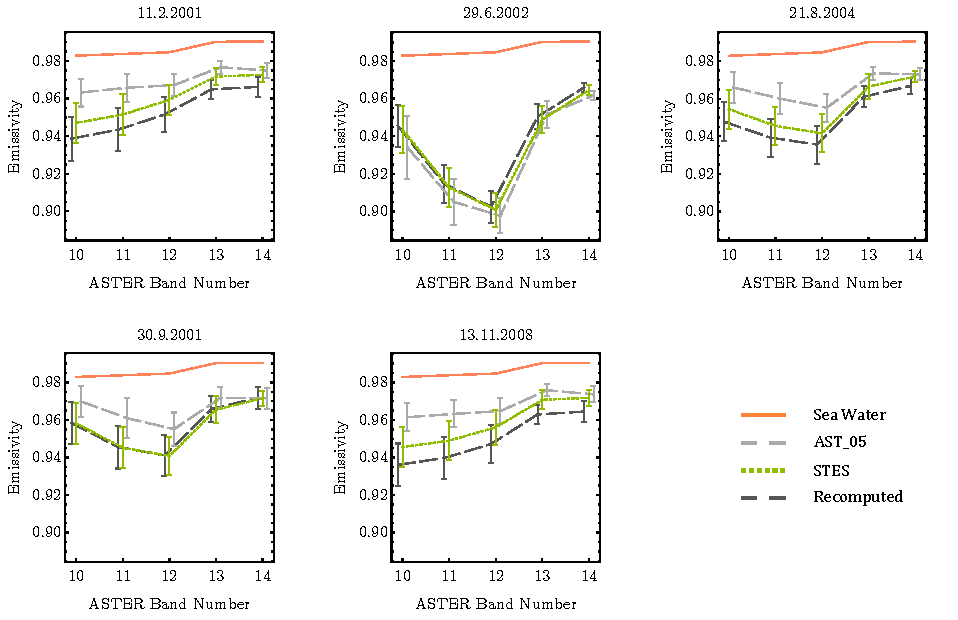
\includegraphics[width=0.98\linewidth]{pics/Chapter_04/Caspian.pdf}
\vspace{1.5 em}
\caption{Emissivity of Caspian Sea in different seasons obtained from the ASTER standard product AST\_05, OSTES retrieval, and emissivity recomputation according to the temperature from AST\_08 and land-leaving and downwelling radiance from AST\_09T. Emissivities were extracted from an area of size $40 \times 40$ pixels over pure and cloudless waterbody. Error bars display standard deviation.}
\label{fig:CaspianSeaEmissivity}
\end{figure*}

\begin{figure}[!h]
\centering
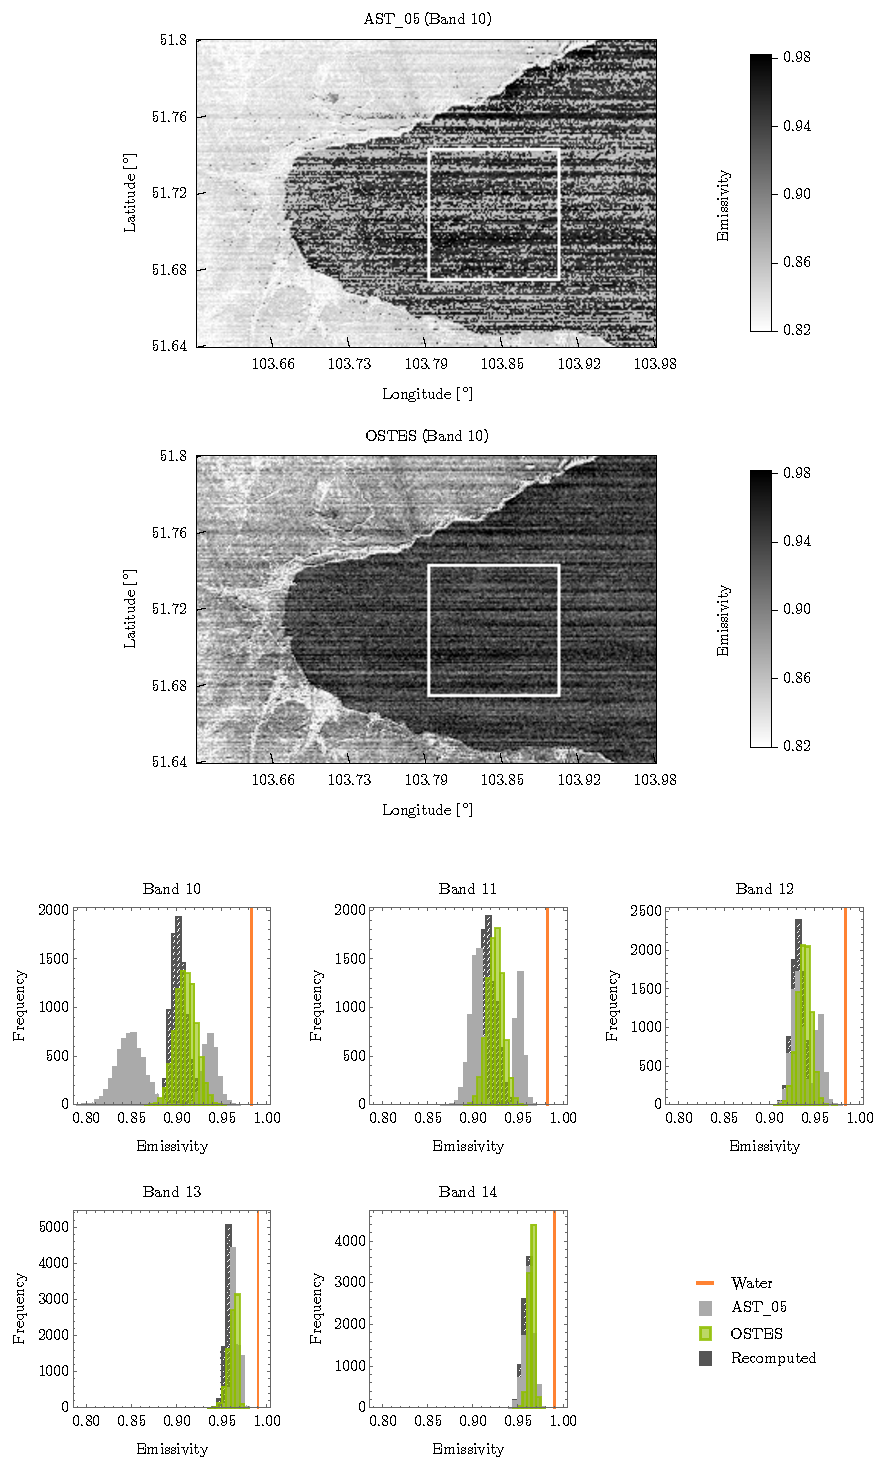
\includegraphics[width=0.76\linewidth]{pics/Chapter_04/Baikal.pdf}
\vspace{1.5 em}
\caption{
ASTER band 10 emissivity images of Lake Baikal obtained from ASTER standard product AST\_05 (top) and OSTES emissivity retrieval (middle). In both images the same contrast stretching is used. The white square represents the area from which emissivity histrograms were created (bottom panel). Histograms show distributions of AST\_05 emissivity, OSTES emissivity and recomputed emissivity according to the temperature from AST\_08 and land-leaving and downwelling radiance from AST\_09T. Vertical line depicted in histograms indicates the expected value of water emissivity retrieved from ASTER spectral library \cite{BH09}.}
\label{fig:Bajkal}
\end{figure}

\subsection*{Lake Baikal}

The difference in emissivity obtained by the two versions of TES is further illustrated in the scene over Lake Baikal shown in Figure \ref{fig:Bajkal}. In this figure the white squares on the images define a water body sample of size $90 \times 90$ pixels that was used to produce the values in the histograms below the images. The expected values of sea water emissivity (red vertical line) are included in the Figure \ref{fig:Bajkal}. The histograms show the OSTES emissivity retrievals compared against the AST\_05 standard product, as well as the emissivity recomputed with respect to the temperature delivered by AST\_08 and land-leaving and downwelling radiance delivered by AST\_09T, as described in the previous paragraph. Inspection of the ASTER standard product AST\_05 shows that emissivity values in bands 10, 11 and 12 over the homogeneous study sample are clustered around two distinct values. This creates step discontinuities which are reflected in the bimodal distributions in the histograms and in the noisy patterns in the left image. This will be discussed further below. In contrast to AST\_05 emissivities, OSTES emissivity results are smoother and the histograms do not show any significant bimodality. The recomputed and OSTES emissivity retrievals are similar. However, the OSTES emissivities tend to be closer to the expected values. In addition to the noise, striping is also visible in the image. Striping is caused by electronic noise and can distort emissivity spectra by triggering thresholds included in the original TES algorithm. This can cause step discontinuities. Temperature retrievals are not significantly affected. Striping is more thoroughly discussed in \cite{GA11}. Even though the AST\_05 and OSTES emissivities differ significantly in some bands, the temperature retrievals are very similar. The average difference is \SI{0.25}{\kelvin} (s.d. \SI{0.18}{\kelvin}). Similar to the discussion regarding Caspian Sea emissivity retrievals, it can also be concluded in this case that none of the emissivity spectra have satisfying values.

\begin{figure}[!t]
\centering
\vspace{0.8 em}
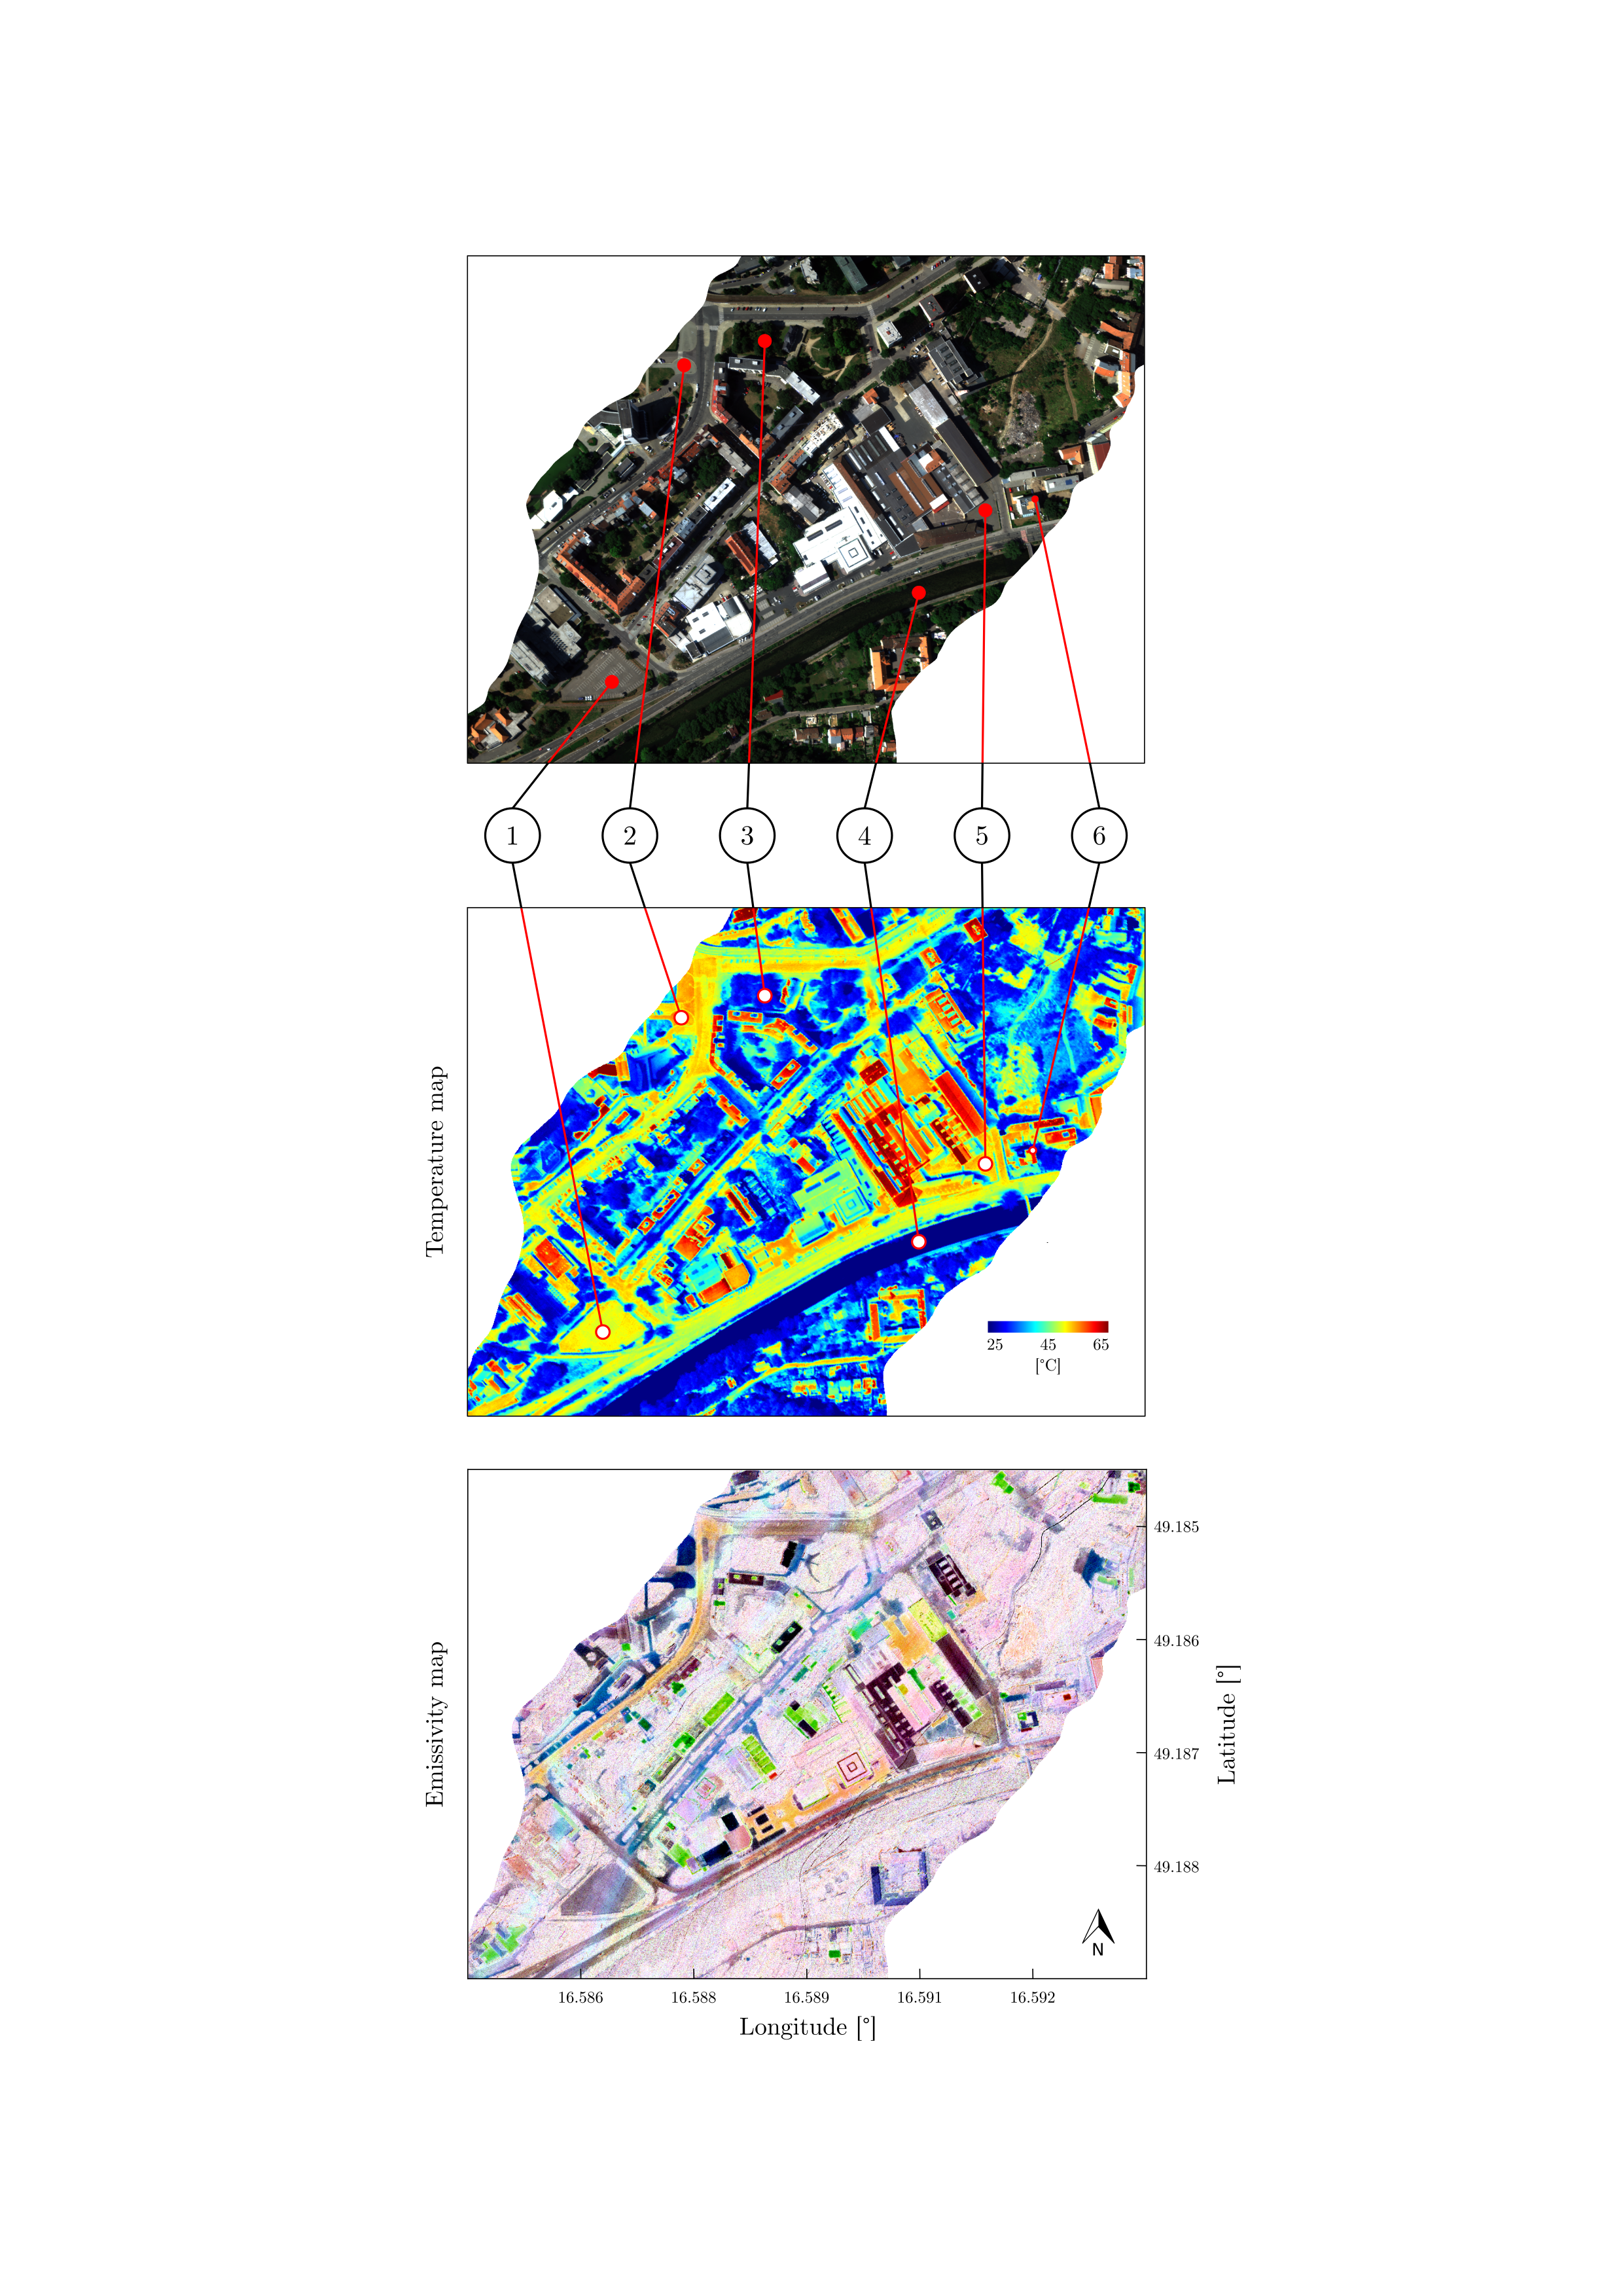
\includegraphics[scale=0.85]{pics/Chapter_04/Brno.pdf}
\vspace{2 em}
\caption{
Part of flight line over the city of Brno. Image data were acquired on 4.7.2015 at 14:03 (UTC). The top image displays RGB composition of the studied area. The middle image depicts temperature map obtained from OSTES algorithm applied on image data from TASI sensor. The bottom image is false color emissivity map obtained from OSTES algorithm (red - band 10, green - band 15, blue - band 20). On the top and middle images are shown locations and labels \textit{in-situ} measurements.}
\label{fig:Brno}
\end{figure}

The discrepancies in shape and magnitude of emissivity spectra can be the result of various source of errors but the main error source has been attributed to imperfect atmospheric corrections \cite{TP01, TP05}. Table \ref{table:ASTERScenes} indicates the amount of precipitable water in the atmosphere for each of the investigated scenes. These values were obtained from NOAA's Climate Forecast System Reanalysis. It can be observed that discrepancies in emissivity spectra are related to amount of precipitable water in the atmosphere. Notable works discussing emissivity retrievals over agricultural areas and water bodies are \cite{CC07, SJ07}. One suggested improvement is the water vapour scaling method \cite{T05, GA11}.

The step discontinuities in emissivity values over homogeneous areas can occur due to various thresholds deciding how to treat the sample during processing. The original TES algorithm starts in the NEM module assuming a maximum emissivity spectra $\varepsilon_\mathrm{max}=0.99$. The NEM module is then restarted with refined $\varepsilon_\mathrm{max}$ according to the emissivity retrieved from the first NEM pass. When the NEM iterations do not converge, then the correction for downwelling radiance is not possible, and obtained values of temperature and emissivity are reported as final. The original version of TES processes samples according to the MMD of emissivity spectra obtained from the NEM module either by incorporating (\ref{eq:MMD}) or by presetting emissivity to $\varepsilon = 0.983$. Some authors \cite{GG06}, \cite{SG09} have suggested that the value of the threshold used for classifying observations into groups with either low or high spectral contrast should be changed or completely removed. Observations with wrongly determined spectral contrast or observations with spectral contrast close to any threshold result in step discontinuities. On the contrary, the OSTES does not set any thresholds for materials with low spectral contrast and so it is expected to generate smoother results on homogeneous areas with low spectral contrast.

\section{Application to TASI Image Data}

The OSTES algorithm was applied on image data acquired by TASI sensor and the results were compared with emissivities obtained from \textit{in-situ} mesaurements and the TES algorithm esmissivity estiamtions. 

\subsection*{Experiment Setup}

The study was performed using data acquired over the city of Brno, Czech Republic (lat: 49.2, lon: 16.6). The examined data are subset of a flight line crossing the city from south-west to north-east. The acquisition was performed on 4.7.2015 at 14:03 (UTC). The FLIS operated by Global Change Research Institute CAS (Brno, Czech Republic) \cite{HF14} was used for this acquisition. FLIS consists of Compact Airborne Spectrographic Imager (CASI), Shortwave infrared Airborne Spectrographic Imager (SASI) and TASI sensor. All sensors are developed by Itres Ltd. (Calgary, Canada).

Within this study were performed \textit{in-situ} measurements of urban materials with Fourier transform infrared (FTIR) Spectrometer Models 102 developed by D\&P Instruments (Simsbury, USA). The emissivity of measured surfaces was estimated by a spectral smoothing algorithm \cite{HJ98}. Emissivity spectra of water and deciduous trees were not measured but instead they were extracted from ASTER spectral library \cite{BH09}. All emissivity spectra were resampled with respect to TASI response functions. The study area and locations of the \textit{in-situ} measurements are shown in the upper part of the Figure \ref{fig:Brno}. 

Spectral emissivity libraries are very useful for calibration and validation purposes. Let us emphasize that there are many other spectral emissivity libraries available apart from ASTER spectral library. Notable libraries are Johns Hopkins University Spectral Library \cite{SW91}, Arizona State University Spectral Library \cite{CB00}, United States Geological Survey Spectral Library \cite{CS16} and the Spectral Library of Urban Materials (SLUM) \cite{KS14}. In the Appendix \ref{app:Library} is described a spectral emissivity library which is specifically focused on spoil substrates.

\subsection*{The OSTES implementation to the TASI Processing Chain}

Image data acquired by the TASI sensor were radiometrically, atmospherically and gemetrically pre-processed as described in the Chapter~\ref{chap:Data}. The result of the pre-processing is land-leaving radiance, which is the first input parameter for the OSTES and the TES algorithm. The second input parameter to the both algorithms is downwelling atmospheric radiance. This quantity was obtained from radiative transfer model MODTRAN~\cite{BG06}. The input to MODTRAN requires temperature and water vapour profiles, which were extracted from MOD07\_L2 product~\cite{B11} generated from MODIS image data.

The described procedure of the temperature and emissivity estimation from the pre-processed TASI image data is the continuation of the processing chain introduced in the Chapter~\ref{chap:Data}. The schematic illustration of the OSTES implementation into the processing chain of the TASI image data is depicted in the Figure~\ref{fig:OSTESProcessingChain}, which is the continuation of the processing chain depicted in the Figure~\ref{fig:ProcessingChain}. The whole processing chain of TASI image data described in this work is operational at Global Change Research Institute CAS (Brno, Czech Republic).

\begin{figure}[thb]
	\centering
	\vspace{0.7 em}
	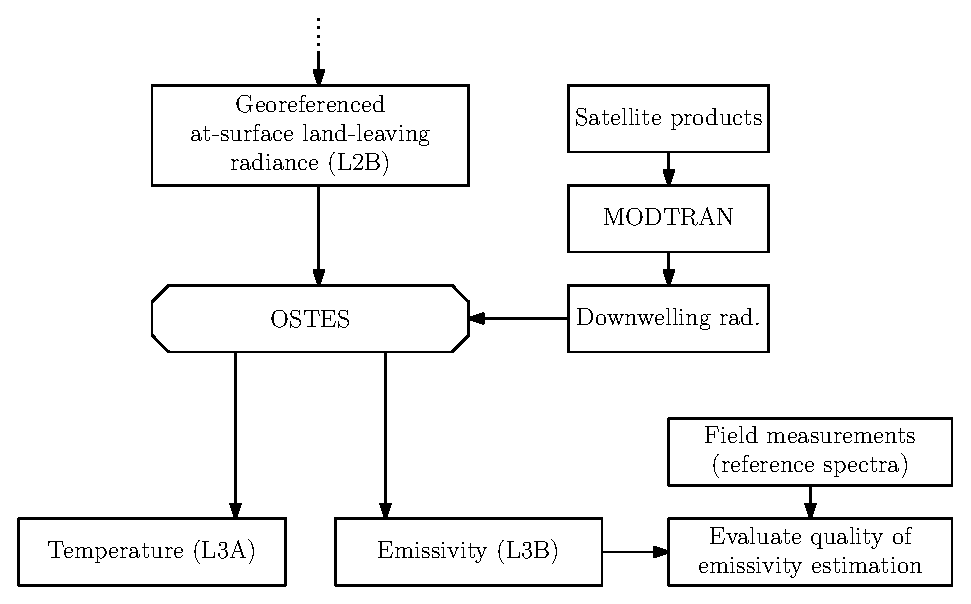
\includegraphics[scale=1]{pics/Chapter_04/OSTES_processing_chain.eps}
	\vspace{2 em}
	\caption{Continuation of the processing chain of the TASI image data introduced in the Chapter \ref{chap:Data} and depicted in the Figure \ref{fig:ProcessingChain}. This part illustrates temperature and emissivity separation processing chain applied to the pre-processed TASI image data.}
	\label{fig:OSTESProcessingChain}
	\vspace{0.7 em}
\end{figure}

The processing of the TASI image data acquired during this experiment was limited to 22 spectral bands. First five and last five spectral bands were not considered since they were affected by imperfect atmospheric corrections.

The TASI image data were processed by the TES and OSTES algorithms in order to~compare the temperature and emissivity retrievals. The TASI image data were processed with the TES algorithm by substituting OSTES algorithm in the processing chain of~TASI image data. The implementation of the TES algorithm is based on the implementation described in~the \cite{JS12} without the $\varepsilon_\mathrm{max}$ refinement for emissivities with low spectral contrast.
 
\subsection*{Comparison}

Temperature and emissivity results of the OSTES algorithm are depicted in the middle and lower part of Figure \ref{fig:Brno} in the form of a temperature and emissivity map. The temperature map shows high temperature differences between vegetated and built areas. Emissivity map is a false color composition (red - band 10, green - band 15, blue - band 20) showing variability of surface materials in the image data.

\newpage
The \textit{in-situ} measurements were not performed during the overflight. Therefore temperature could not be used for the comparison and the validation of the TES and OSTES algorithms. The comparison of the TES and the OSTES algorithms' performance was tested against six emissivities obtained from \textit{in-situ} measurements. Results are shown in the Figure \ref{fig:BrnoEmissivityComparison} below, where error bars display standard deviation. Both TES and OSTES emissivity retrievals are very similar. The OSTES performs slightly better than TES in cases of deciduous trees and Svratka River. However, none of these two spectra agrees with the shape and magnitude of the expected emissivity spectra. These discrepancies can be caused by various sources of errors but the main error source has been attributed to the imperfect atmospheric corrections. Emissivities of the spot 5, asphalt parking lots, retrieved by the TES and OSTES significantly differ from \textit{in-situ} measurement. This shift in magnitude is introduced by the insufficient compensation of the downwelling radiance. This spot is surrounded by buildings, which increase the amount of downwelling radiance. This additional radiance is not included in the atmospheric parameters retrieved from MODTRAN. The rest of the emissivity retrievals are considered to follow \textit{in-situ} measurements well. Let us emphasize the reader that OSTES offers only moderate improvements in emissivity retrievals. These are not possible to observe in this comparison due to the magnitude of the error introduced by the imperfect atmospheric corrections. 

These data were acquired within a campaign focused on detecting urban heat island of the city of Brno. The main goal was determination of parameters affecting temperatures in the city. Preliminary observations are introduced in the Appendix \ref{app:Visualisation}.

\begin{figure}[!t]
\centering
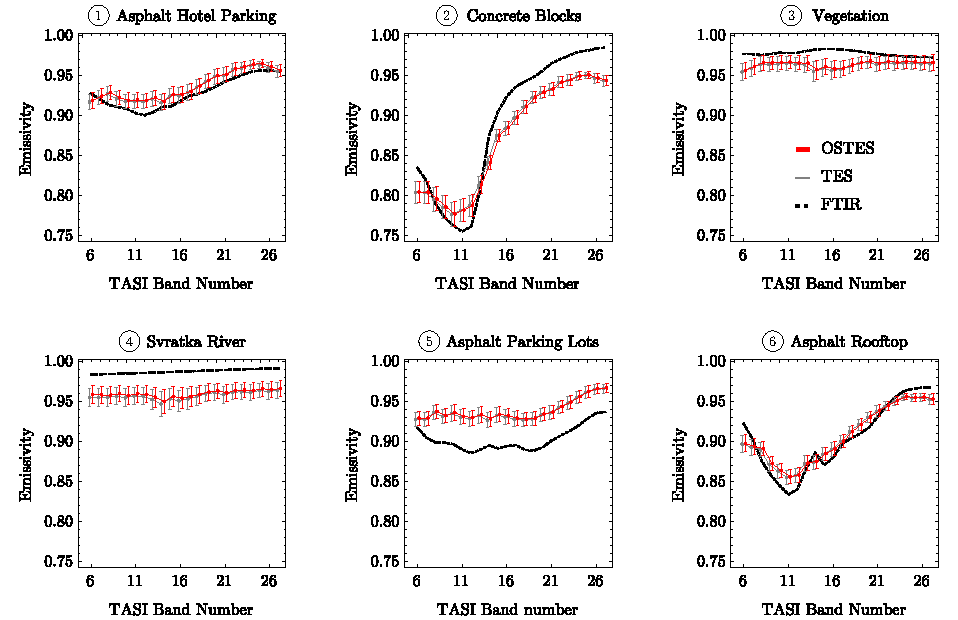
\includegraphics[width=\linewidth]{pics/Chapter_04/Brno-Emissivity-Comparison.pdf}
\vspace{1.5 em}
\caption{Comparison of TES and OSTES emissivity retrievals with emissivities obtained from \textit{in-situ} measurements. Error bars display standard deviation.}
\label{fig:BrnoEmissivityComparison}
\end{figure}




	\cleardoublepage
	\pagestyle{mystyle}
\chapter{Ground Measurements}

\section{Introduction}

Post-mining sites represent areas of large-scale and intensive disturbance. They have serious impact on the surrounding landscape in many countries of the world. Original ecosystems are destroyed, and the restoration of ecosystem functions and services is necessary \cite{BH01}. Afforestation is widely used reclamation method. Many studies demonstrate that post-mining sites have a large potential for carbon sequestration if afforestation has been applied \cite{VF13, FL13, SL05, UL06}. This can contribute to mitigate the increase in atmospheric $\mathrm{CO_2}$ concentrations.

During opencast mining a large amount of substrate above the coal layer is removed and relocated in heaps covering extensive areas. These heaps consist of material often excavated from depths of several hundred meters. This material is called spoil substrate and it can vary in its physical and chemical properties. The heterogeneity is largely affected by geology and the method of mining and heaping. For this reason the substrates differ substantially from recent soils. They often have extreme pH and may contain high concentrations of heavy metals, polyphenols (i.e., products of coal decomposition) and salt content. Such properties can significantly impact a success and/or speed of vegetation development at post mining sites. Therefore a proper knowledge on spoil substrate properties and distribution is necessary in land rehabilitation. 

Thermal remote sensing can provide beneficial tools for monitoring of post-mining areas. Particularly, land surface emissivity (LSE) can be used for spoil substrates classification. In addition, physical and chemical properties can be estimated by spectral analysis of LSE. Land surface temperature (LST) is closely connected to soil moisture which is important for establishment of new ecosystems.

LST is coupled with LSE and thus one quantity cannot be derived without knowledge of the second. These quantities cannot be explicitly derived from radiance measurement. The reason is that by observing radiance in N bands one gets N unknown emissivities plus one unknown temperature. Such a system of equations is underdetermined (i.e., more unknown than known variables). Several algorithms have been suggested to solve this problem \cite{LT13}. These algorithms either require knowledge of LSE in advance, or an estimate LSE as a part of their output. A library of spectral emissivities can be utilized for: 1) determination of LST, 2) material classification, and 3) LSE validation of airborne and satellite thermal remote sensing data.

This work describes a spectral library of spoil substrate emissivities from brown coal mining sites in the Czech Republic near towns of Sokolov, Chodov, Bílina and Ustí nad Labem (Fig. \ref{fig:SpoilSubstratesMap}). The spectral library contains emissivities, soil pH in water and in KCl, soil conductivity, content of water soluble Na and K, Al and Fe in KCl, loss on ignition and content of polyphenols. In addition to all measured physical and chemical parameters, sample’s latitude and longitude are listed. The dataset consists of 24 spoil substrate samples, which were homogenized by mixing and sieving before any sample analysis. The toxicity test and measurement of chemical properties are discussed at length in \cite{FK05}. Data collection for emissivity retrievals was performed outdoors in Petri dishes using a Fourier transform infrared (FTIR) spectrometer Model 102 (D\&P Instruments, United States). The emissivity of each sample was estimated by a spectral smoothing algorithm \cite{HJ98}.

\begin{figure*}[!t]
\centering
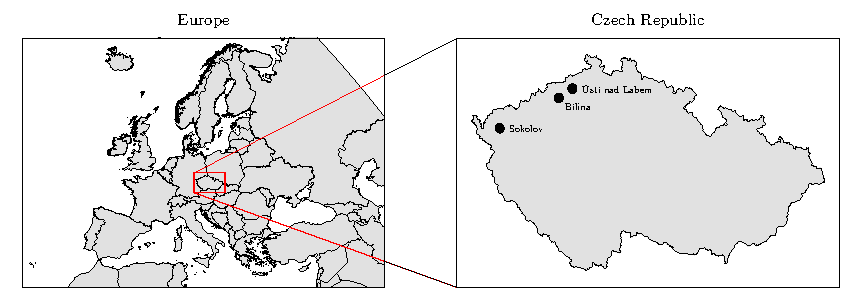
\includegraphics[width=0.95\linewidth]{pics/Chapter_05/map.pdf}
\vspace{1.5 em}
\caption{Locations of brown coal mining sites from which spoil substrate samples were extracted.}
\label{fig:SpoilSubstratesMap}
\end{figure*}

Datasets containing LSE are rare in comparison with datasets containing LST measurements. The most well-known spectral libraries containing emissivities are the ASTER Spectral Library \cite{BH09}, Johns Hopkins University Spectral Library \cite{SW91}, Arizona State University Spectral Library \cite{CB00}, United States Geological Survey Spectral Library \cite{CS16} and the Spectral Library of Urban Materials (SLUM) \cite{KS14}. However, these spectral libraries do not include neither geographical coordinates of samples nor representatives of spoil substrates. One example of a spectral library of emissivities from calibration/validation sites containing coordinates for each sample is described in \cite{SM09}. The dataset described in this paper is exceptional in its nature and location. 

The data presented in this paper were used in a study focused on mapping of spoil substrates for site re-cultivation \cite{Z14} as well as in a study discussing spoil substrates toxicity \cite{FK05}. The mining site was also mapped with the Airborne Hyperspectral Scanner (AHS) in visible, near infrared, shortwave infrared and longwave infrared regions for mineral classification purposes \cite{NK14}. Examples of emissivity spectra retrieved from AHS and their corresponding samples spectra extracted from the library are depicted in Fig. \ref{fig:AHSvsFTIRcomparison}. Samples spectra from the library were spectrally resampled with respect to AHS response functions using weighted averages \cite{LT13}. Comparison of retrieved spectra in case of samples 11 and 19 shows good agreement in shape. Sample 12 exhibit deviations mainly between bands 3 and 4 (9.24 and 9.68 µm). This can be explained by the fact that AHS pixel has 5x5 m pixel size and these pixels were not pure thus had more complex mineral composition than the collected samples. Discrepancies in magnitude can be addressed to imperfect atmospheric corrections or to different soil state during overflight.

\begin{figure}[!t]
	\centering
	\vspace{1em}
	\begin{subfigure}[t]{.3\linewidth}
		\centering
		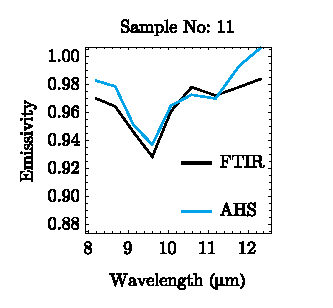
\includegraphics[scale=1]{pics/Chapter_05/Sample_no_11.eps}
		\caption{}
	\end{subfigure}
	\hspace{1em}
	\begin{subfigure}[t]{.3\linewidth}
		\centering
		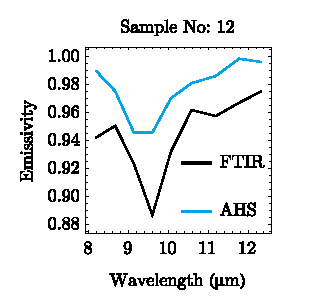
\includegraphics[scale=1]{pics/Chapter_05/Sample_no_12.eps}
		\caption{}
	\end{subfigure}
	\hspace{1em}
	\begin{subfigure}[t]{.3\linewidth}
		\centering
		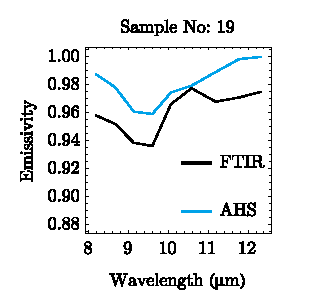
\includegraphics[scale=1]{pics/Chapter_05/Sample_no_19.eps}
		\caption{}
	\end{subfigure}
	\vspace{1.5 em}
	\caption{Examples of corresponding emissivity spectra retrieved from AHS and from spectral library of spoil substrates’. Emissivity spectra from the library were measured by FTIR and they were resampled with respect to AHS response functions. }
	\label{fig:AHSvsFTIRcomparison}
\end{figure}

Any activity involving remote sensing over these mining sites can benefit from publicly releasing the spectral library of spoil substrates emissivity. Apart from remote sensing application, data in spectral library can be further analyzed for identifying relationships between a sample’s spectral emissivity and its chemical properties.

TODO: Data are describe in appendix A and library itself is part supplementary file of article...

\section{Methods}

The study area is situated around two post mining districts: 1) Sokolov – coal-mining district near towns of Sokolov and Chodov (North-West Czech Republic) and 2) North Czech coal mining district near towns of Bílina and Ustí nad Labem (North Czech Republic). Open-pit mines produce large areas of tailings where spoil material was sampled. Claylike tertiary sediments dominate in these districts.

Spoil substrates were sampled from bare soil without vegetation. Samples contained negligible amounts of organic matter. Extracted samples were further homogenized by mixing and sieving trough a 2 mm screen. Homogenized samples were divided into two groups, from which the first one was used for chemical analysis and the second one for toxicity testing. Samples set for chemical analysis were air dried and stored in a dark place at room temperature. Soil pH in water and in 1N KCl (which is 74.56 g of potassium chloride diluted in 1000 mL of water \cite{J03}) was measured using a pH meter with glass electrode in suspension. The suspension was prepared in 1:5 spoil to water ratio and 1:5 spoil to KCl ratio. Conductivity was measured in filtrated suspension using a conductometer. The suspension was prepared in 1:5 spoil to water ratio. Content of water soluble Na and K was also measured in filtrated water suspension (1:5 spoil to water ratio) using an ion selective electrode. Both suspensions were left to stay overnight. Al and Fe contents in 1N KCl eluate, (1:5 spoil to water ratio), were determined by spectrophotometer Spectra AA 640 (Varian, Australia). Loss on ignition was measured by burning spoil samples at 600 °C for 5 h. This process is called ashing. To determine the amount of polyphenols samples were kept in 80\% ethanol (1:5 spoil to ethanol ratio) and stayed for 24 h. Samples were then filtrated and the polyphenol content was determined spectrophotometrically by Folin–Ciocalteau reagent at a wavelength of 765 nm \cite{HL97}. Gallic acid was used as a standard for calibration. The polyphenol content was expressed as mg/100 g of soil. Toxicity was determined by enchytraeid toxicity test. The test is based on the population growth of pot worms in substrates. The details of the measurement are discussed in \cite{FK05}.

Spoil substrates emissivity measurements were collected with Designs and Prototypes Model 102 (United States) portable FTIR spectrometer. The measurement was performed outdoor under clear sky conditions during two consecutive days in summer season. The spectroradiometer was pre-heated to maximum expected ambient day temperature during the nights before both measurement days. Spectrometer orientation during measurements was south to avoid shadows. Fore-optics field-of-view was 4.8° and it was 60 cm away from the sample. Such a configuration resulted in spot size of approximately 5 cm. Samples were put in Petri dish of diameter 14 cm and they were let to be heated up naturally by sunlight. Samples temperatures ranged from 40 °C to 50 °C. Every sample was measured at three different spots. The measurement of one spot consists of ten measurements, which were averaged. The resulting emissivity of each sample is the average of all three measurements. Sample temperature and emissivity were determined by a spectral smoothing algorithm, as described in \cite{HJ98}.

During the measurements the instrument was calibrated using two blackbodies at different temperatures. A cold blackbody was set to ambient temperature (30 °C) and warm blackbody was set just above the sample temperature (40 – 50 °C). The calibration procedure during first four spoil samples was done between the changing of each sample. The calibration procedure during the rest of the measurements was done between every fourth sample. Before every sample a measurement was made of a diffuse gold reflectance plate (Infragold from Labsphere Inc.), to compensate for downwelling radiance, as suggested in \cite{GV13}. The measurement of one sample along with instrument calibration and measurement of the diffuse gold reflectance plate took around 15 minutes. A description of the procedures for converting instrument response to radiance and compensating for downwelling radiance can be found in \cite{HJ98} and \cite{HK96}.

Some of the spoil substrate emissivity spectra are greater than one at certain wavelengths. This inaccuracy occurs at both ends of provided wavelengths interval (i.e. near 8 µm and near 14 µm). Data at these wavelengths are on the edge of atmospheric window and thus the cause of the inaccuracy is imperfect compensation for downwelling radiance. Samples with numbers 33, 34 and 38 are missing header information of latitude and longitude. Absent values are indicated by ‘NA’ string. In these cases the origin of the sample is specified with respect to closest town (either Bílina or Sokolov). We still find these data meaningful, since they can be used as spectral endmembers.


\section{Data Properties}

All samples are claylike sediments which imply that spectral features of clay can be found in every emissivity spectra. Fig. \ref{fig:SpectraPreview} depicts three examples of spoil samples taken from the spectral library. Sample 02 (Fig. \ref{fig:SpectraPreview}a) is clay consisting mostly of kaolinite with significant peaks at 8.90, 9.50, and 10.00 µm. Sample 06 (Fig. \ref{fig:SpectraPreview}b) is coal combined with sand and clay. The emissivity spectrum of this sample contains kaolinite features mixed with a quartz feature at 8.50, 8.90, 9.30 and 10.00 µm. The sample 33 (Fig. \ref{fig:SpectraPreview}c) is bentonite rich for montmorillonite. Montmorillonite has typical dip in spectral emissivity at 9.43 µm. The spectral emissivity library of spoil substrates includes also image providing a preview of all samples in library similar to images shown in Figure 3.

\begin{figure}[!t]
	\centering
	\vspace{1em}
	\begin{subfigure}[t]{.3\linewidth}
		\centering
		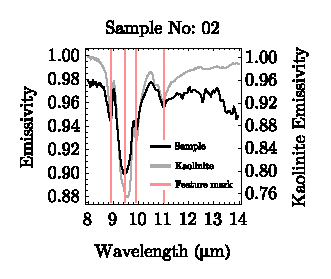
\includegraphics[scale=1]{pics/Chapter_05/Sample_no_02.eps}
		\caption{}
	\end{subfigure}
	\hspace{1em}
	\begin{subfigure}[t]{.3\linewidth}
		\centering
		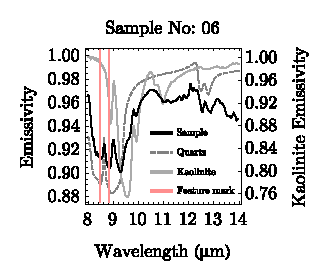
\includegraphics[scale=1]{pics/Chapter_05/Sample_no_06.eps}
		\caption{}
	\end{subfigure}
	\hspace{1em}
	\begin{subfigure}[t]{.3\linewidth}
		\centering
		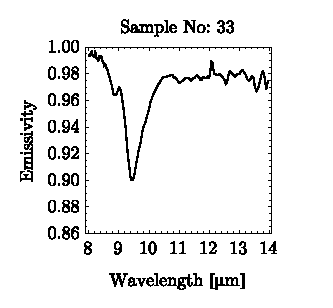
\includegraphics[scale=1]{pics/Chapter_05/Sample_no_33.eps}
		\caption{}
	\end{subfigure}
	\vspace{1.5 em}
	\caption{Spectra of three samples taken from the spectral emissivity library of spoil substrates: (a) sample 02 representing clay rich for kaolinite; (b) sample 06 representing coal combined with sand and clay; (c) sample 33 representing bentonite. }
	\label{fig:SpectraPreview}
\end{figure}

Thermal remote sensing can be used for classification of spoil substrates and for determination of their physical and chemical properties. The spectral library presented in this paper can ease and enhance all these activities. Obtained information together with LST are valuable for selection and monitoring of restoration process on post-mining sites.

\section{Spectral Smoothing Algorithm}




%% zaver
	\cleardoublepage
	\pagestyle{myzaver}
\chapter{Conclusion}

The TES algorithm is well established and popular for several reasons: it retrieves temperature and emissivity of natural surfaces simultaneously without any previous knowledge of surface type and it is widely applicable to range of multispectral and hyperspectral sensors. This suggests that the algorithm is a good benchmark for temperature and emissivity separation. \textcolor{red}{Any improvement to the TES algorithm} can benefit \textcolor{red}{processing of thermal data} from many sources.

This work introduced a module that estimates temperature and emissivity from an approximation of the relationship between brightness temperature and emissivity. The new module replaces the NEM module in the original TES to create an algorithm we call OSTES. The performance of OSTES was firstly tested on a set of simulated data recomputed with respect to ASTER, AHS and TASI response functions. Results show that temperature estimations using OSTES are more accurate and precise than TES for samples with low spectral contrast. It should be noted that this improvement is of modest size when compared to the already accurate results that can be obtained with TES. OSTES and TES perform similarly for samples with a high spectral contrast. The results also reveal that OSTES is less sensitive to  variations in atmospheric conditions.

The OSTES was also \textcolor{red}{compared against the} ASTER standard product AST\_09T over the Caspian Sea and Lake Baikal. By comparing the OSTES results to ASTER standard products AST\_08 (temperature) and AST\_05 (emissivity) we found that temperature retrievals of both algorithms are very close. However, it was also found that temperatures included in AST\_08 product are not consistent with emissivities delivered by AST\_05 product in the sense of (\ref{eq:emissivityComputation}). Thus emissivities were recomputed based on downwelling and land-leaving radiance from AST\_09T and temperature from AST\_08. Comparing all three emissivity retrievals over  {the} Caspian Sea in different seasons shows that emissivity from AST\_05 to be closest and recomputed emissivity to be the furthest from expected sea water emissivity values extracted from ASTER Spectral Library, except in the June  {and September scenes}, which  {are} expected to have the largest water vapour burden in the atmosphere. It is also observed that the AST\_05 emissivities over Lake Baikal exhibit step discontinuities. In the same region OSTES and recomputed emissivities tend to be smoother with OSTES emissivities being closer to expected value of water emissivity. All emissivity retrievals are probably affected by inaccurate atmospheric corrections since none of the obtained spectra had emissivity values close to expected values.

We conclude that improvements in atmospheric compensation will be crucial for further improvements in emissivity results. Thus, further work should be focused on this topic. We believe it is important to validate the performance of future improvements by using data acquired by a variety of multispectral and hyperspectral sensors, such as AHS and TASI. Additional improvements in OSTES will consider modifications of cost function represented in (\ref{eq:costFunction}) and illustrated in Fig. \ref{fig:FunctionCode}. Better approximations of the relationship between brightness temperature and emissivity could result in better temperature and emissvity retrievals. 

Since TES plays important role in the TIR data processing, we suggest to use OSTES instead of TES mainly because of higher precision and accuracy under conditions of low spectral contrast, and because of the consistency between retrieved temperature and emissivity. We hope that improvements introduced by OSTES will help to enhance the quality of temperature and emissivity results.

\cleardoublepage
%% dodatky
\pagestyle{mydodatky}

\begin{appendices}

\chapter{Spectral Emissivity Library of Spoil Substrates}
\label{app:Library}

The spectral library consists of 24 ASCII files. Each file describes one spoil substrate. Individual files are named according to the sample number. Files consist of a file header and spectral emissivities. Both file parts are described in the subsections below.

\section{Header}

The format of header is similar to format of ASTER Spectral Library header \cite{BH09}. Each file contains 26 lines of header, which includes available sample information. The header is divided into four sections separated by empty lines. First part contains 9 lines discussing sample classification, particle size and sample origin. Sample origin is expressed by latitude and longitude on the reference ellipsoid WGS84. This information is summarized in the following fields:

\begin{enumerate}
	\item	Name
	\item Type
	\item Class
	\item Particle size
	\item Sample No
	\item Owner
	\item Origin
	\item Latitude
	\item Longitude
\end{enumerate}

A second section contains information about sample toxicity and chemical properties. The unit of each quantity is indicated in square brackets after quantity name. This header section contains following fields:

\begin{enumerate}
	\item toxicity
	\item pH in H20
	\item pH in KCl
	\item conductivity
	\item water soluble Na
	\item water soluble K
	\item Al in KCl
	\item Fe in KCl
	\item loss on ignition
	\item polyphenol content
\end{enumerate}

A third section contains reference to \cite{FK05}, which discusses toxicity measurement and chemical analysis. Finally, the fourth header section contains the names of two columns, in which the following spectral emissivity data are aligned. Metadata in each header line contains an attribute name followed by a colon (ASCII Character 3A) and tab (ASCII Character 09) and then the corresponding value.

\section{Spectral Emissivity}

After the header part, the file continues on lines 27 – 213 with spectral emissivity data aligned in two columns. As header file indicates, the first column contains wavelength in micrometers and the second column contains corresponding emissivity value. Values in each row are separated by tab. The emissivity of each sample is provided in wavelengths interval from 8 µm to 14 µm. Sampling in this interval is non-linear.

\begin{figure*}[!t]
\centering
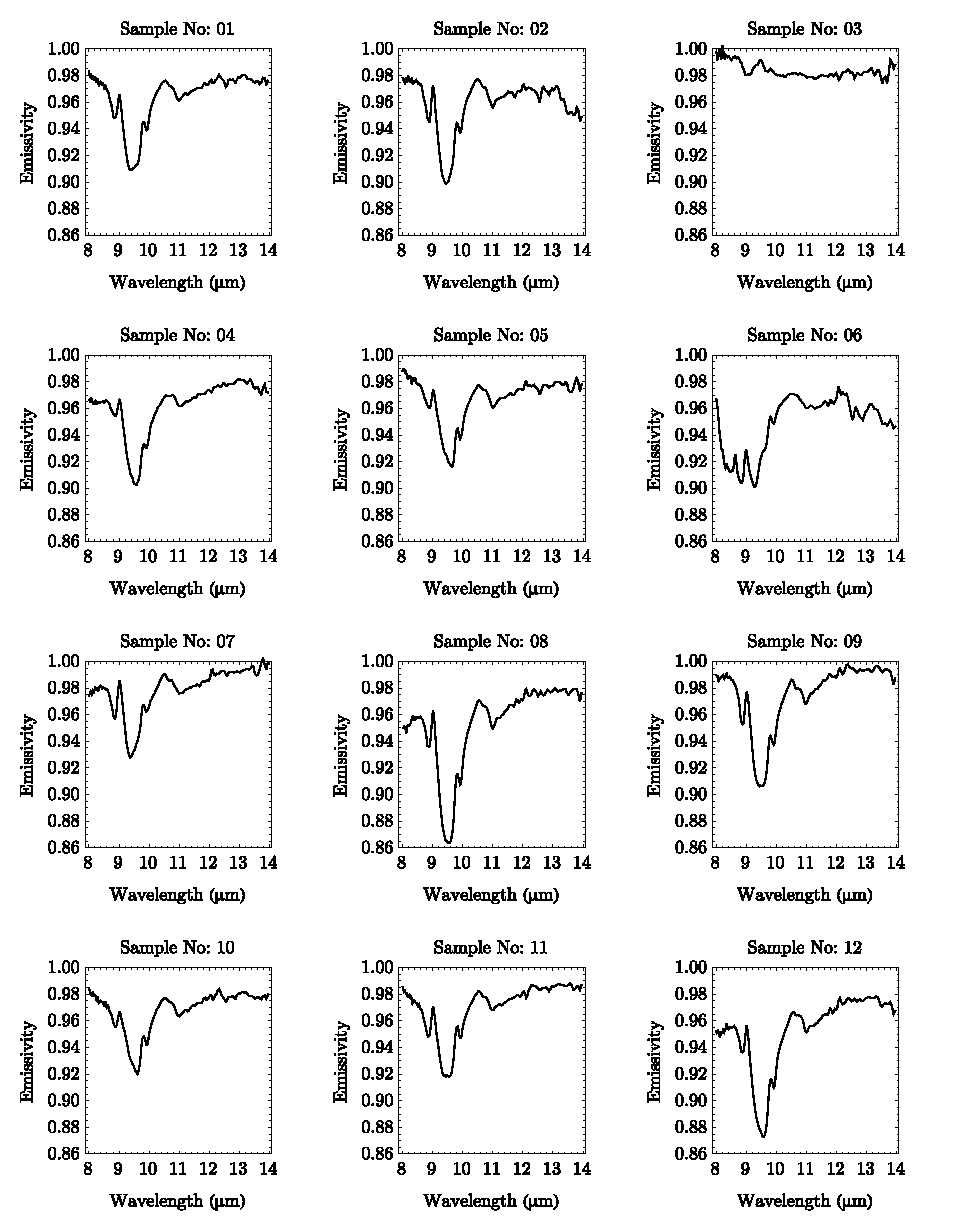
\includegraphics[width=0.95\linewidth]{pics/Chapter_05/spectral_library_pt1.eps}
\vspace{1.5 em}
\caption{TODO.}
\label{fig:SpoilSubstratesPreviewPt1}
\end{figure*}

\begin{figure*}[!t]
\centering
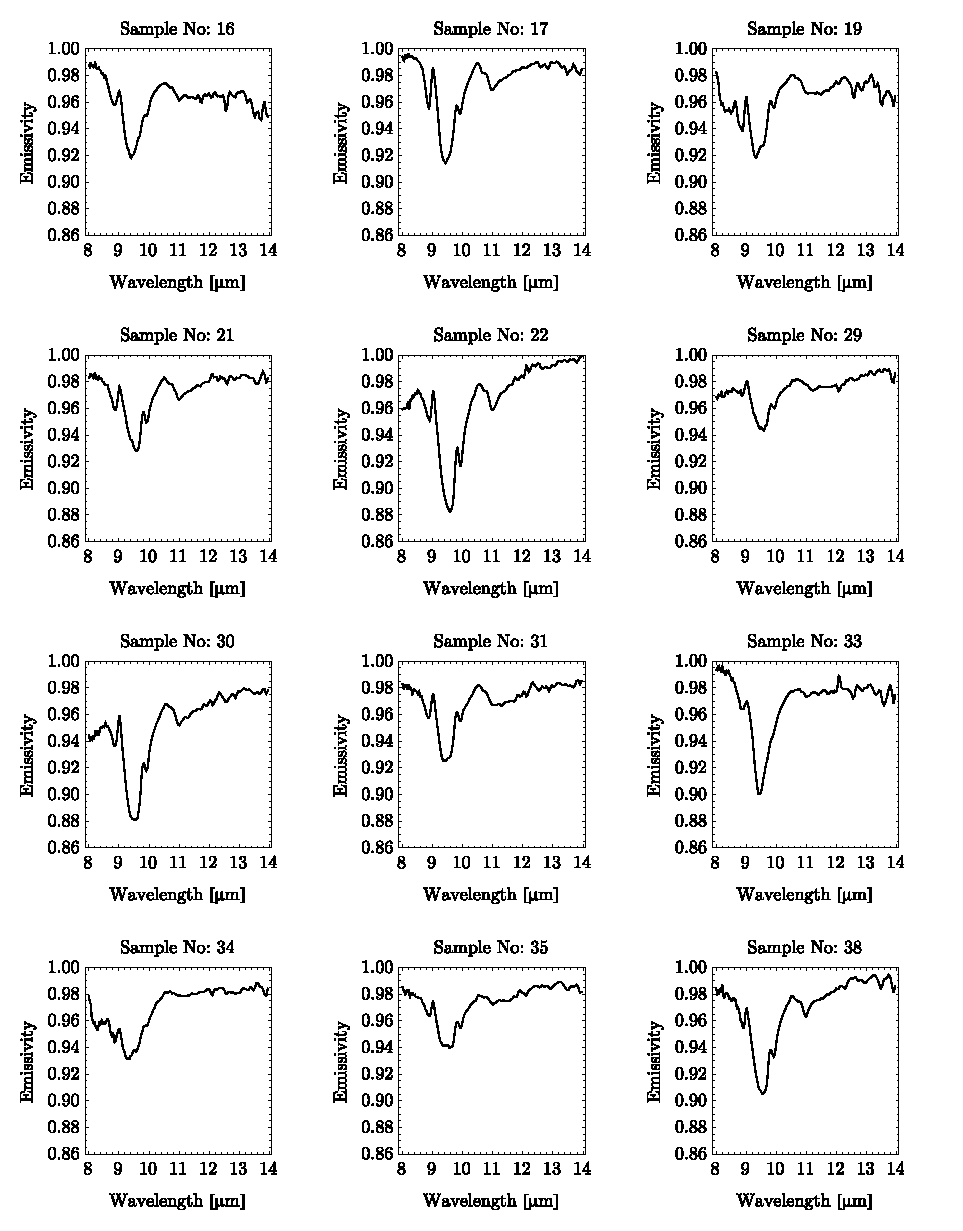
\includegraphics[width=0.95\linewidth]{pics/Chapter_05/spectral_library_pt2.eps}
\vspace{1.5 em}
\caption{TODO.}
\label{fig:SpoilSubstratesPreviewPt1}
\end{figure*}

\begin{appendices}

\chapter{Spectral Emissivity Library of Spoil Substrates}
\label{app:Library}

Spectral emissivity libraries contains valuable information about Earth surface materials, which can be utilised for validation and calibration purposes of airborne or satellite image data. Several libraries are currently available among which is also a spectral emissivity library of spoil substrates \cite{PP16}. This appendix introduces mentioned library in detail.

\section{Introduction}

Post-mining sites represent areas of large-scale and intensive disturbance. They can have significant impacts on the surrounding landscape in many countries of the world. Original ecosystems can be damaged or destroyed, and the restoration of ecosystem functions and services is necessary \cite{BH01}. Afforestation is widely used reclamation method. Many studies demonstrate that post-mining sites have a large potential for carbon sequestration if afforestation has been applied \cite{VF13, FL13, SL05, UL06}. This can contribute to mitigate the current increase in atmospheric $\mathrm{CO_2}$ concentrations.

During opencast mining a large amount of substrate above the coal layer is removed and relocated in heaps covering extensive areas. These heaps consist of material often excavated from depths of several hundred meters. This material is called spoil substrate and it can vary in its physical and chemical properties. The heterogeneity is largely affected by geology and the method of mining and heaping. For this reason the substrates differ substantially from recent soils. They often have extreme pH and may contain high concentrations of heavy metals, polyphenols (i.e., products of coal decomposition) and salt content. Such properties can significantly impact a success and/or speed of vegetation development at post mining sites. Therefore a proper knowledge on spoil substrate properties and distribution is necessary in land rehabilitation. 

Thermal infrared remote sensing can provide beneficial tools for monitoring of post-mining areas. Particularly, land surface emissivity (LSE) can be used for spoil substrates classification. In addition, physical and chemical properties can be estimated by spectral analysis of LSE. Land surface temperature (LST) is closely connected to soil moisture which is important for establishment of new ecosystems. All of this information is required when proper land reclamation should be applied. This can include mainly substrate mechanical treatment, such as trenching in order to regulate water regime, chemical treatment (e.g., liming), and selection of appropriate tree species.

LST is coupled with LSE and thus one quantity cannot be derived without knowledge of the second. These quantities cannot be explicitly derived from radiance measurement. The reason is that by observing radiance in N bands one gets N unknown emissivities plus one unknown temperature. Such a system of equations is underdetermined (i.e., more unknown than known variables). Several algorithms have been suggested to solve this problem \cite{LT13}. These algorithms either require knowledge of LSE in advance, or an estimate LSE as a part of their output. A library of spectral emissivities can be utilized for: 1) determination of LST, 2) material classification, and 3) LSE validation of airborne and satellite thermal remote sensing data.

This work describes a spectral library of spoil substrate emissivities from brown coal mining sites in the Czech Republic near towns of Sokolov, Chodov, Bílina and Ustí nad Labem (Figure \ref{fig:SpoilSubstratesMap}). The spectral library contains emissivities, soil pH in water and in KCl, soil conductivity, content of water soluble Na and K, Al and Fe in KCl, loss on ignition and content of polyphenols. In addition to all measured physical and chemical parameters, sample's latitude and longitude are listed. The dataset consists of 24 spoil substrate samples, which were homogenized by mixing and sieving before any sample analysis. The toxicity test and measurement of chemical properties are discussed at length in \cite{FK05}. Data collection for emissivity retrievals was performed outdoors in Petri dishes using a Fourier transform infrared (FTIR) spectrometer Model 102 (D\&P Instruments, United States). The emissivity of each sample was estimated by a spectral smoothing algorithm \cite{HJ98}.

\begin{figure*}[!t]
\centering
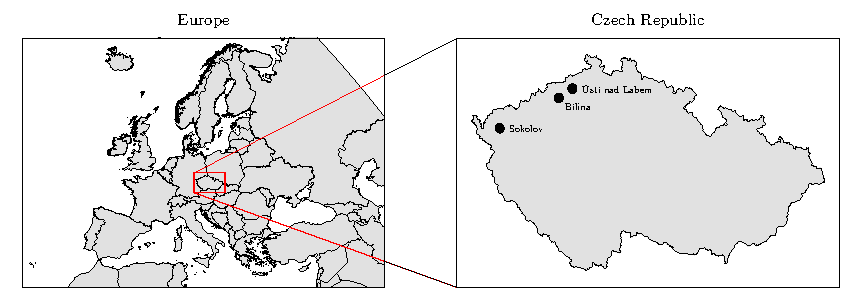
\includegraphics[width=0.95\linewidth]{pics/Chapter_05/map.pdf}
\vspace{1.5 em}
\caption{Locations of brown coal mining sites from which spoil substrate samples were extracted.}
\label{fig:SpoilSubstratesMap}
\end{figure*}

Datasets containing LSE are rare in comparison with datasets containing LST measurements. The most well-known spectral libraries containing emissivities are the ASTER Spectral Library \cite{BH09}, Johns Hopkins University Spectral Library \cite{SW91}, Arizona State University Spectral Library \cite{CB00}, United States Geological Survey Spectral Library \cite{CS16} and the Spectral Library of Urban Materials (SLUM) \cite{KS14}. However, these spectral libraries do not include neither geographical coordinates of samples nor representatives of spoil substrates. One example of a spectral library of emissivities from calibration/validation sites containing coordinates for each sample is described in \cite{SM09}. The dataset described in this paper is exceptional in its nature and location. 

The data presented in this paper were used in a study focused on mapping of spoil substrates for site re-cultivation \cite{Z14} as well as in a study discussing spoil substrates toxicity \cite{FK05}. The mining site was also mapped with the Airborne Hyperspectral Scanner (AHS) in visible, near infrared, shortwave infrared and longwave infrared regions for mineral classification purposes \cite{NK14}. Examples of emissivity spectra retrieved from AHS and their corresponding samples spectra extracted from the library are depicted in Figure \ref{fig:AHSvsFTIRcomparison}. Samples spectra from the library were spectrally resampled with respect to AHS response functions using weighted averages \cite{LT13}. Comparison of retrieved spectra in case of samples 11 and 19 shows good agreement in shape. Sample 12 exhibits deviations mainly between bands 3 and 4 (9.24 and \SI{9.68}{\micro\meter}). This can be explained by the fact that AHS pixel has 5x5 m pixel size and these pixels were not pure thus had more complex mineral composition than the collected samples. Discrepancies in magnitude can be addressed to imperfect atmospheric corrections or to different soil state during overflight.

\begin{figure}[!t]
	\centering
	\vspace{1em}
	\begin{subfigure}[t]{.3\linewidth}
		\centering
		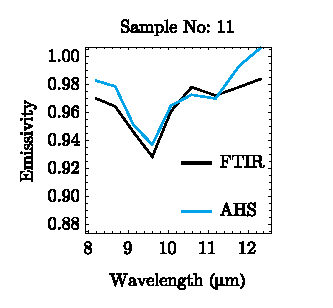
\includegraphics[scale=1]{pics/Chapter_05/Sample_no_11.eps}
		\caption{}
	\end{subfigure}
	\hspace{1em}
	\begin{subfigure}[t]{.3\linewidth}
		\centering
		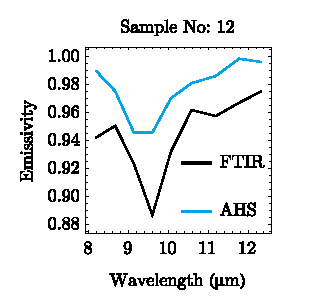
\includegraphics[scale=1]{pics/Chapter_05/Sample_no_12.eps}
		\caption{}
	\end{subfigure}
	\hspace{1em}
	\begin{subfigure}[t]{.3\linewidth}
		\centering
		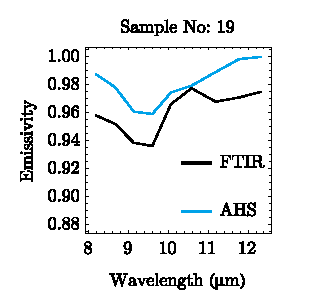
\includegraphics[scale=1]{pics/Chapter_05/Sample_no_19.eps}
		\caption{}
	\end{subfigure}
	\vspace{1.5 em}
	\caption{Examples of corresponding emissivity spectra retrieved from AHS and from spectral library of spoil substrates’. Emissivity spectra from the library were measured by FTIR and they were resampled with respect to AHS response functions. }
	\label{fig:AHSvsFTIRcomparison}
\end{figure}

Any activity involving remote sensing over these mining sites can benefit from publicly releasing the spectral library of spoil substrates emissivity. Apart from remote sensing application, data in spectral library can be further analyzed for identifying relationships between a sample’s spectral emissivity and its chemical properties.

\section{Methods}

The study area is situated around two post mining districts: 1) Sokolov – coal-mining district near towns of Sokolov and Chodov (North-West Czech Republic) and 2) North Czech coal mining district near towns of Bílina and Ustí nad Labem (North Czech Republic). Open-pit mines produce large areas of tailings where spoil material was sampled. Claylike tertiary sediments dominate in these districts.

Spoil substrates were sampled from bare soil without vegetation. Samples contained negligible amounts of organic matter. Extracted samples were further homogenized by mixing and sieving trough a \SI{2}{\milli\meter} screen. Homogenized samples were divided into two groups, from which the first one was used for chemical analysis and the second one for toxicity testing. Samples set for chemical analysis were air dried and stored in a dark place at room temperature. Soil pH in water and in 1N KCl (which is \SI{74.56}{\gram} of potassium chloride diluted in \SI{1000}{\milli\liter} of water \cite{J03}) was measured using a pH meter with glass electrode in suspension. The suspension was prepared in 1:5 spoil to water ratio and 1:5 spoil to KCl ratio. Conductivity was measured in filtrated suspension using a conductometer. The suspension was prepared in 1:5 spoil to water ratio. Content of water soluble Na and K was also measured in filtrated water suspension (1:5 spoil to water ratio) using an ion selective electrode. Both suspensions were left to stay overnight. Al and Fe contents in 1N KCl eluate, (1:5 spoil to water ratio), were determined by spectrophotometer Spectra AA 640 (Varian, Australia). Loss on ignition was measured by burning spoil samples at \SI{600}{\celsius} for \SI{5}{\hour} h. This process is called ashing. To determine the amount of polyphenols, samples were kept in 80\,\% ethanol (1:5 spoil to ethanol ratio) and stayed for \SI{24}{\hour}. Samples were then filtrated and the polyphenol content was determined spectrophotometrically by Folin–Ciocalteau reagent at a wavelength of \SI{765}{\nano\meter} \cite{HL97}. Gallic acid was used as a standard for calibration. The polyphenol content was expressed as \SI{}{\milli\gram\per 100\gram} of soil. Toxicity was determined by enchytraeid toxicity test. The test is based on the population growth of pot worms in substrates. The details of the measurement are discussed in \cite{FK05}.

Spoil substrate emissivity measurements were collected with Designs and Prototypes Model 102 (United States) portable FTIR spectrometer. The measurements were performed outdoors under clear sky conditions during two consecutive days in the summer season. The spectroradiometer was pre-heated to maximum expected ambient day temperature during the nights before both measurement days. The samples were positioned on the south side of the spectrometer to avoid shadows. The fore-optic field-of-view was \SI{4.8}{\degree} and it was \SI{60}{\centi\meter} from the sample. Such a configuration resulted in a spot size of approximately 5 cm. Samples were put in a \SI{14}{\centi\meter} diameter Petri dish and were allowed to be heated up naturally in the sunlight. Sample temperatures ranged from \SI{40}{\celsius} to \SI{50}{\celsius}. Every sample was measured at three different spots. The measurement of one spot consisted of ten measurements, which were averaged. The resulting emissivity of each sample is the average of all three measurements. Sample temperature and emissivity were determined by a spectral smoothing algorithm, as described in \cite{HJ98}.

During the measurements the instrument was calibrated using two blackbodies at different temperatures. A cold blackbody was set to the ambient temperature (\SI{30}{\celsius}) and warm blackbody was set just above the sample temperature (40 -- \SI{50}{\celsius}). The calibration procedure during the first four spoil samples was done between the changing of each sample. The calibration procedure during the rest of the measurements was done between every fourth sample. Before every sample a measurement was made of a diffuse gold reflectance plate (Infragold from Labsphere Inc.), to compensate for downwelling radiance, as suggested in \cite{GV13}. The measurement of one sample along with instrument calibration and measurement of the diffuse gold reflectance plate took around 15 minutes. A description of the procedures for converting instrument response to radiance and compensating for downwelling radiance can be found in \cite{HJ98} and \cite{HK96}.

Some of the spoil substrate emissivity spectra are greater than one at certain wavelengths. This inaccuracy occurs at both ends of provided wavelengths interval (i.e. near \SI{8}{\micro\meter} and near \SI{14}{\micro\meter}). Data at these wavelengths are on the edge of atmospheric window and thus the cause of the inaccuracy is imperfect compensation for downwelling radiance. Samples with numbers 33, 34 and 38 are missing header information of latitude and longitude. Absent values are indicated by ‘NA’ string. In these cases the origin of the sample is specified with respect to closest town (either Bílina or Sokolov). We still find these data meaningful, since they can be used as spectral endmembers.


\section{Data Properties}

All of the samples contain varying amounts and types of clay minerals, as evidenced by their spectral emissivity features. Figure \ref{fig:SpectraPreview} depicts three examples of spoil samples taken from the spectral library. These spectra can be compared with spectra of similar materials extracted from Arizona State University Spectral Library \cite{CB00} and ASTER Spectral Library \cite{BH09}, which are illustrated in the Figure \ref{fig:SpectraPreview} as well. Sample 02 (Figure \ref{fig:SpectraPreview}a) is clay consisting mostly of kaolinite with significant dips at 8.90, 9.44, 9.90, and \SI{11.00}{\micro\meter}. Sample 06 (Figure \ref{fig:SpectraPreview}b) is coal combined with sand and clay. The emissivity spectrum of this sample contains kaolinite features mixed with a quartz feature at 8.47 and \SI{8.83}{\micro\meter}. The sample 33 (Figure \ref{fig:SpectraPreview}c) is bentonite rich for montmorillonite. Montmorillonite has typical dip in spectral emissivity at \SI{9.43}{\micro\meter}. The spectral emissivity library of spoil substrates includes also image providing a preview of all samples in library similar to images shown in Figure \ref{fig:SpectraPreview}.

\begin{figure}[!t]
	\centering
	\vspace{1em}
	\begin{subfigure}[t]{.3\linewidth}
		\centering
		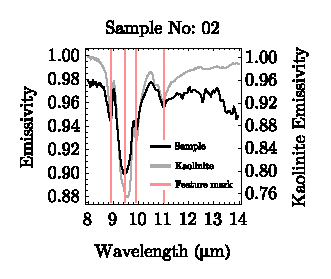
\includegraphics[scale=1]{pics/Chapter_05/Sample_no_02.eps}
		\caption{}
	\end{subfigure}
	\hspace{1em}
	\begin{subfigure}[t]{.3\linewidth}
		\centering
		\includegraphics[scale=1]{pics/Chapter_05/Sample_no_06.eps}
		\caption{}
	\end{subfigure}
	\hspace{1em}
	\begin{subfigure}[t]{.3\linewidth}
		\centering
		\includegraphics[scale=1]{pics/Chapter_05/Sample_no_33.eps}
		\caption{}
	\end{subfigure}
	\vspace{1.5 em}
	\caption{Spectra of three samples taken from the spectral emissivity library of spoil substrates: (a) sample 02 representing clay rich for kaolinite; (b) sample 06 representing coal combined with sand and clay; (c) sample 33 representing bentonite. Kaolinite and montmorillonite spectra were extracted from Arizona State University Spectral Libary \cite{CB00} and quartz spectra was extracted from ASTER Spectral Library \cite{BH09}. Kaolinite spectrum is scaled for clarity reasons.}
	\label{fig:SpectraPreview}
\end{figure}

Thermal infrared remote sensing can be used for classification of spoil substrates and for determination of their physical and chemical properties. The spectral library presented in this paper can ease and enhance all these activities. Obtaining this information together with LST is valuable for selection and monitoring of restoration process at post-mining sites. 

\section{Data Description}

The spectral library consists of 24 ASCII files. Each file describes one spoil substrate. Individual files are named according to the sample number. Files consist of a file header and spectral emissivities. Both file parts are described in the subsections below.

\subsection{Header}

The format of the header is similar to the format of the ASTER Spectral Library header \cite{BH09}. Each file contains 26 lines of header, which includes available sample information. The header is divided into four sections separated by empty lines. First part contains 9 lines discussing sample classification, particle size and sample origin. Sample origin is expressed by latitude and longitude on the reference ellipsoid WGS84. This information is summarized in the following fields:

\begin{enumerate}
	\item	Name
	\item Type
	\item Class
	\item Particle size
	\item Sample No
	\item Owner
	\item Origin
	\item Latitude
	\item Longitude
\end{enumerate}

A second section contains information about sample toxicity and chemical properties. The unit of each quantity is indicated in square brackets after quantity name. This header section contains following fields:

\begin{enumerate}
	\item toxicity
	\item pH in H20
	\item pH in KCl
	\item conductivity
	\item water soluble Na
	\item water soluble K
	\item Al in KCl
	\item Fe in KCl
	\item loss on ignition
	\item polyphenol content
\end{enumerate}

A third section contains reference to \cite{FK05}, which discusses toxicity measurement and chemical analysis. Finally, the fourth header section contains the names of two columns, in which the following spectral emissivity data are aligned. Metadata in each header line contains an attribute name followed by a colon (ASCII Character 3A) and tab (ASCII Character 09) and then the corresponding value.

\subsection{Spectral Emissivity}

After the header part, the file continues on lines 27 – 213 with spectral emissivity data aligned in two columns. As header file indicates, the first column contains wavelength in micrometers and the second column contains corresponding emissivity value. Values in each row are separated by tab. The emissivity of each sample is provided in wavelengths interval from \SI{8}{\micro\meter} to \SI{14}{\micro\meter}. Sampling in this interval is non-linear. Spectral emissivities contained in the spectral library are depicted in Figures \ref{fig:SpoilSubstratesPreviewPt1} and \ref{fig:SpoilSubstratesPreviewPt2}. Spectral emissivity library is part of the supplementary materials to the manuscript \cite{PP16}.

\begin{figure*}[!t]
\centering
\includegraphics[width=0.95\linewidth]{pics/Chapter_05/spectral_library_pt1.eps}
\vspace{1.5 em}
\caption{Depiction of samples' emissivity spectra included in the library of spoil substrates.}
\label{fig:SpoilSubstratesPreviewPt1}
\end{figure*}

\begin{figure*}[!t]
\centering
\includegraphics[width=0.95\linewidth]{pics/Chapter_05/spectral_library_pt2.eps}
\vspace{1.5 em}
\caption{Depiction of samples' emissivity spectra included in the library of spoil substrates.}
\label{fig:SpoilSubstratesPreviewPt2}
\end{figure*}

%%%%%%%%%%%%%%%%%%%%%%%%%%%%%%%%%%%%%%%%%%%%%%%%%%%%%%%%%%%%%%%%%
%% literatura
	\cleardoublepage
	\pagestyle{mybiblio}
\begin{thebibliography}{10}
\addcontentsline{toc}{chapter}{Bibliography}
%\makeatletter
%\def\@biblabel#1{}
%\let\old@bibitem\bibitem
%\def\bibitem#1{\old@bibitem{#1}\leavevmode\kern-\bibindent}
%\makeatother

%\footnotesize

\section*{Author’s publications}
%%%%%%%%%%%%%%%%%%%%%%%%%%%%%%%%%%%%%%%%%%%%%%%%%%%%%%%%%%%%%%%%%%%%%%%%%%%%%%%%%%%%%%%%%%%%%%%%%%%

\bibitem{PP16} PIVOVARNÍK, M., PIKL, M., FROUZ, J., ZEMEK, F., KOPAČKOVÁ, V., NOTESCO, G. and BEN DOR, E. A Spectral Emissivity Library of Spoil Substrates. \textit{Data}. 2016, \textbf{1}(12). DOI: 10.3390/data1020012

\bibitem{NP16} NOVOTNÝ, J., PIVOVARNÍK, M., KHALSA, S.J. and ZEMEK, F. Visualisation of dependencies between city structure and thermal behaviour in Brno. \textbf{In:} \textit{23rd International Archives of the Photogrammetry, Remote Sensing and Spatial Information Sciences Congress, ISPRS 2016}. Prague, 2016, 741-745. DOI: 10.5194/isprsarchives-XLI-B2-741-2016.

\bibitem{JP14} JANOUTOVÁ, R., PIVOVARNÍK, M. Modelling of spruce trees using L-systems. \textbf{In:} \textit{20th International Conference on Soft Computing: Evolutionary Computation, Genetic Programming, Swarm Intelligence, Fuzzy Logic, Neural Networks, Fractals, Bayesian Methods, MENDEL 2014.} Brno, 2014, 153-158. ISSN: 18033814. 

% MOJE PUBLIKACE
%\bibitem{hf_ibcst} Holešovský, J., Fusek, M. (2015). Metody analýzy extrémních hodnot a~jejich softwarová implementace. Odesláno k~publikaci.
%%
%\bibitem{hfm_hsj} Holešovský, J., Fusek, M., Blachut, V., Michálek, J. (2015). Comparison of precipitation extremes estimation using parametric and nonparametric methods. \emph{Hydrological Sciences Journal}. Přijato k~publikaci. DOI 10.1080/02626667.2015.1111517.
%%
%\bibitem{hfm1} Holešovský, J., Fusek, M., Michálek, J. (2015). Modelling of precipitation extremes using parametric and nonparametric methods with automated threshold selection. \emph{International Journal of Mathematics and Computers in Simulation} \textbf{9}, 94-102.
%%
%\bibitem{hfm_recko} Holešovský, J., Fusek, M., Michálek, J. (2014). Automated threshold selection for parametric and non-parametric estimates of intensity-duration-frequency curves. \emph{Proceedings of the 1st International Conference on Mathematical Methods \& Computational Techniques in Science \& Engineering, MMCTSE 2014}. Athens, Greece. ISBN 987-1-61804-256-9.
%%
%\bibitem{hfm_mendel} Holešovský, J., Fusek, M., Michálek, J. (2014). Extreme value estimation for correlated observations. \emph{20th International Conference on Soft Computing MENDEL 2014.} Brno, Czech Republic, 359-364.
%%
%\bibitem{hp_pdmu} Holešovský, J., Popela, P. (2012). Stochastic Extensions of a~Traffic Assignment Problem. \emph{XX International Conference PDMU-2012: Problems of Decision Making under Uncertainties, Proceeding - Applied Papers.} Brno, Czech Republic, 61-70. ISBN 978-80-7231-897-1.
%%
%\bibitem{hpr_mendel} Holešovský, J., Popela, P., Roupec, J. (2013). Disruption in Congested Networks. \emph{Proceedings of 19th International Conference on Soft Computing MENDEL 2013.} Brno, Czech Republic, 191-196. ISBN 978-80-214-4755-4.
%%
%\bibitem{hz_ryby} Olejníčková, Z., Holešovský, J., Vávrová, M., Králová, Z., Michálek, J. (2014). Methylmercury in tissues of fish from the Svratka River, the Czech Republic. \emph{Fresenius Environmental Bulletin} \textbf{23}(12b), 3319-3324.
%%
%\bibitem{hs_zizaly} Škarková, P., Zlámalová Gargošová, H., Holešovský, J., Vávrová, M., Michálek, J., Olejníčková, Z. (2015). Application of statistical methods for ecotoxicological data evaluation. \emph{Fresenius Environmental Bulletin} \textbf{24}(5), 1692-1698.

\subsection*{Scientifically less trustable references}

%%%%%%%%%%%%%%%%%%%%%%%%%%%%%%%%%%%%%%%%%%%%%%%%%%%%%%%%%%%%%%%%%%%%%%%%%%%%%%%%%%%%%%%%%%%%%%%%%%%

\section*{Other references}

%\addcontentsline{toc}{section}{References}

\bibitem{B15}
B.~Eng, personal communication, 2015.

\bibitem{BH09} BALDRIDGE, A.M., HOOK, S.J., GROVE, C.I. and RIVERA, G. The ASTER spectral library version 2.0. \textit{Remote Sensing of Environment}. 2009, \textbf{113}(4), 711-715. DOI: 10.1016/j.rse.2008.11.007.

\bibitem{BP96} BARDUCCI, A. and PIPPI, I. Temperature and emissivity retrieval from remotely sensed images using the "Grey body emissivity" method. \textit{IEEE Transactions on Geoscience and Remote Sensing}. 1996, \textbf{34}(3), 681-695. DOI: 10.1109/36.499748.

\bibitem{BG06} BERK, A., ANDERSON, G.P., ACHARYA, P.K., BERNSTEIN, L.S., MURATOV, L., LEE, J., FOX, M., ADLER-GOLDEN, S.M., CHETWYND, J.H., HOKE, JR. M.L., LOCKWOOD, R.B., GARDNER, J.A., COOLEY, T.W., BOREL, C.C., LEWIS, P.E. and SHETTLE, E.P. MODTRAN5: 2006 update. \textbf{In:} \textit{Algorithms and Technologies for Multispectral, Hyperspectral, and Ultraspectral Imagery XII}. Orlando (Kissimmee), FL, 2006, F2331--F2331. DOI: 10.1117/12.665077.

\bibitem{B11} BORBAS, E., SEEMANN, S.W., KERN, A., MOY, L., LI, J., GUMLEY, L. and MENZEL, W.P. \textit{MODIS Atmospheric Profile Retrieval - ATBD} [online]. 2011. [cit. 2016-08-10]. Available at: http://modis-atmos.gsfc.nasa.gov/\_docs/MOD07\_atbd\_v7\linebreak\_April2011.pdf

\bibitem{B98} BOREL, C. Surface emissivity and temperature retrieval for a hyperspectral sensor. \textbf{In:} \textit{IGARSS '98. Sensing and Managing the Environment. 1998 IEEE International Geoscience and Remote Sensing. Symposium Proceedings. (Cat. No.98CH36174).} Seattle, WA: IEEE, 1998, 546-549. DOI: 10.1109/IGARSS.1998.702966.

\bibitem{B08} BOREL, C. Error analysis for a temperature and emissivity retrieval algorithm for hyperspectral imaging data. \textit{International Journal of Remote Sensing} [online]. 2008, \textbf{29}(17-18), 5029-5045. DOI: 10.1080/01431160802036540.

\bibitem{BH01} BRADSHAW, A.D. and HÜTTL, R.F. Future minesite restoration involves a broader approach. Ecological Engineering. 2001, \textbf{17}(2-3), 87-90. DOI: 10.1016/S0925-8574(00)00149-X. ISSN 09258574.

\bibitem{CC98} CHEVALLIER, F., CHÉRUY, F., SCOTT, N.A. and CHÉDIN, A. A neural network approach for a fast and accurate computation of a longwave radiative budget. \textit{Journal of Applied Meteorology}. 1998, \textbf{37}(11), 1385-1397. DOI: 10.1175/1520-0450(1998)037<1385:ANNAFA>2.0.CO;2.

\bibitem{CS85} CHÉDIN, A., SCOTT, N.A., WAHICHE, C. and MOULINIER, P. The improved initialization inversion method: a high resolution physical method for temperature retrievals from satellites of the TIROS-N series. \textit{Journal of Climate and Applied Meteorology}. 1985, \textbf{24}(2), 128-143. DOI: 10.1175/1520-0450(1985)024<0128:TIIIMA>2.0.CO;2

\bibitem{CB00} CHRISTENSEN, P.R., BANDFIELD, J.L., HAMILTON, V.E., HOWARD, D.A., LANE, M.D., PIATEK, J.L., RUFF, S.W. and STEFANOV, W.L. A thermal emission spectral library of rock-forming minerals. \textit{Journal of Geophysical Research: Planets}. 2000, \textbf{105}(E4), 9735-9739. DOI: 10.1029/1998JE000624.

\bibitem{CS16} CLARK, R.N., SWAYZE, G.A., WISE, R., LIVO, E., HOEFEN, T., KOKALY, R., SUTLEY, S.J. \textit{USGS digital spectral library splib06a} [online]. U.S. Geological Survey, Digital Data Series 231, 2007. [cit. 2016-07-12]. Available at: http://speclab.cr.usgs.gov/spectral.lib06

\bibitem{CC07} COLL, C., CASELLES, V., VALOR, E., NICLÒS, R., SÁNCHEZ, J.M., GALVE, J.M. and MIRA, M. Temperature and emissivity separation from ASTER data for low spectral contrast surfaces. \textit{Remote Sensing of Environment}. 2007, \textbf{110}(2), 162-175. DOI: 10.1016/j.rse.2007.02.008. 

\bibitem{FM05} FERNÁNDEZ-RENAU, A., MEYNART, R., NEECK, S.P., GÓMEZ, J.A., DE MIGUEL, E. and SHIMODA, H. The INTA AHS system. \textbf{In:} \textit{SPIE Proceedings}. Bruges: SPIE, 2005, 471-478. DOI: 10.1117/12.629440.

\bibitem{FK05} FROUZ, J., KRIŠTŮFEK, V., BASTL, J., KALČÍK, J. and VAŇKOVÁ, H. Determination of Toxicity of Spoil Substrates After Brown Coal Mining Using a Laboratory Reproduction Test with Enchytraeus crypticus (Oligochaeta). \textit{Water, Air, \& Soil Pollution}. 2005, \textbf{162}(1-4), 37-47. DOI: 10.1007/s11270-005-5991-y. 

\bibitem{FL13} FROUZ, J., LIVEČKOVÁ, M., ALBRECHTOVÁ, J., CHROŇÁKOVÁ, A., CAJTHAML, T., PIŽL, V., HÁNĚL, L., STARÝ, J., BALDRIAN, P., LHOTÁKOVÁ, Z., ŠIMÁČKOVÁ, H. and CEPÁKOVÁ, Š. Is the effect of trees on soil properties mediated by soil fauna? A case study from post-mining sites. \textit{Forest Ecology and Management}. 2013, \textbf{309}, 87-95. DOI: 10.1016/j.foreco.2013.02.013.

\bibitem{GV13} GARCIA-SANTOS, V., VALOR, E., CASELLES, V., MIRA, M., GALVE, J.M. a COLL, C. Evaluation of Different Methods to Retrieve the Hemispherical Downwelling Irradiance in the Thermal Infrared Region for Field Measurements. \textit{IEEE Transactions on Geoscience and Remote Sensing}. 2013, \textbf{51}(4), 2155-2165. DOI: 10.1109/TGRS.2012.2209891.

\bibitem{G86} GILLESPIE, A.R., \textit{Lithologic mapping of silicate rocks using TIMS} [online]. Jet Propulsion Lab., California Inst. of Tech., Pasadena, CA, United States, 1986. [cit. 2016-08-10]. Available at: http://ntrs.nasa.gov/search.jsp?R=19870007685

\bibitem{GA11} GILLESPIE, A.R., ABBOTT, E.A., GILSON, L., HULLEY, G., JIMÉNEZ-MUÑOZ, J.C. and SOBRINO, J.A. Residual errors in ASTER temperature and emissivity standard products AST08 and AST05. \textit{Remote Sensing of Environment}. 2011, \textbf{115}(12), 3681-3694. DOI: 10.1016/j.rse.2011.09.007.

\bibitem{GR99} GILLESPIE, A.R., ROKUGAWA, S., HOOK, S., MATSUNAGA, T. and KAHLE, A.B. \textit{Temperature/Emissivity Separation Algorithm Theoretical Basis Document, Version 2.4} [online]. Pasadena: Jet Propulsion Laboratory, 1999. [cit. 2016-01-19]. Available at: http://eospso.nasa.gov/sites/default/files/atbd/atbd-ast-05-08.pdf 

\bibitem{GR98} GILLESPIE, A.R., ROKUGAWA, S., MATSUNAGA, T., COTHERN, J.S., HOOK, S. and KAHLE, A.B. A temperature and emissivity separation algorithm for Advanced Spaceborne Thermal Emission and Reflection Radiometer (ASTER) images. \textit{IEEE Transactions on Geoscience and Remote Sensing}. 1998, \textbf{36}(4), 1113-1126. DOI: 10.1109/36.700995.

\bibitem{GG00} GU, D., GILLESPIE, A.R., KAHLE, A.B. and PALLUCONI, F.D. Autonomous atmospheric compensation (AAC) of high resolution hyperspectral thermal infrared remote-sensing imagery. \textit{IEEE Transactions on Geoscience and Remote Sensing}. 2000, \textbf{38}(6), 2557-2570. DOI: 10.1109/36.885203.

\bibitem{GG06} GUSTAFSON, W.T., GILLESPIE, A.R. and YAMADA, G.J. Revisions to the ASTER temperature/emissivity separation algorithm. \textbf{In:} \textit{Second Recent Advances in Quantitative Remote Sensing}. Valencia, 2006, 770-775.

\bibitem{HF14} HANUŠ, J., FABIÁNEK, T., KAPLAN, V. and HOMOLOVÁ, L. Flying laboratory of imaging systems (FLIS) at CzechGlobe. \textbf{In:} \textit{SGEM2014 Conference Proceedings}. 2014, 177-182. DOI: 10.5593/SGEM2014/B23/S10.022. ISBN 978-619-7105-12-4. ISSN 1314-2704.

\bibitem{HL97} HAMOUZ, K., LACHMAN, J., PIVEC, V. and ORSÁK, M. The effect of the conditions of cultivation on the content of polyphenol compounds in the potato varieties Agria and Karin. \textit{Rostlinná Výroba}. 1997, \textbf{43}, 541-546.

\bibitem{HK96} HOOK, S.J. and KAHLE, A.B. The micro fourier transform interferometer (uFTIR) — A new field spectrometer for acquisition of infrared data of natural surfaces. \textit{Remote Sensing of Environment}. 1996, \textbf{56}(3), 172-181. DOI: 10.1016/0034-4257(95)00231-6.

\bibitem{HJ98} HORTON, K.A., JOHNSON, J.R. and LUCEY, P.G. Infrared Measurements of Pristine and Disturbed Soils 2. Environmental Effects and Field Data Reduction. Remote Sensing of Environment. 1998, \textbf{64}(1), 47-52. DOI: 10.1016/S0034-4257(97)00167-3.

\bibitem{H11} HOWELL, J.R. \textit{Thermal radiation heat transfer}. 5th ed. Boca Raton: CRC Press, c2011. 957. ISBN 978-1-4398-0533-6.

\bibitem{HH11} HULLEY, G. and HOOK, S.J. Generating Consistent Land Surface Temperature and Emissivity Products Between ASTER and MODIS Data for Earth Science Research. \textit{IEEE Transactions on Geoscience and Remote Sensing}. 2011, \textbf{49}(4), 1304-1315. DOI: 10.1109/TGRS.2010.2063034.

\bibitem{HH11-2}  HULLEY, G. and HOOK, S.J. \textit{HyspIRI Level-2 Thermal Infrared (TIR) Land Surface Temperature and Emissivity Algorithm Theoretical Basis Document} [online]. Pasadena, California: Jet Propulsion Laboratory, California Institute of Technology, 2011. [cit. 2016-01-19]. Available at: https://hyspiri.jpl.nasa.gov/downloads/Algorithm\_Theoretical\_Basis/HyspIRI\_L2\linebreak\_Surface\_Temperature\_Emissivity\_JPL\_Pub\_11-5\_10102011.pdf

\bibitem{software:SparCal} ITRES. SparCal [software]. [access  1.3.2016]. Available at: http://www.itres.com\linebreak/supporting-products/

\bibitem{software:RCX} ITRES. RCX [software]. [access 1.3.2016]. Available at: http://www.itres.com\linebreak/supporting-products/

\bibitem{software:GCSS} ITRES. GCSS [software]. [access 1.3.2016]. Available at: http://www.itres.com\linebreak/supporting-products/

\bibitem{JC09} JIMÉNEZ-MUÑOZ, J.C., CRISTOBAL, J., SOBRINO, J.A., SORIA, G., NINYEROLA, M. and PONS, X. Revision of the Single-Channel Algorithm for Land Surface Temperature Retrieval From Landsat Thermal-Infrared Data. \textit{IEEE Transactions on Geoscience and Remote Sensing}. 2009, \textbf{47}(1), 339-349. DOI: 10.1109/TGRS.2008.2007125.

\bibitem{JS12} JIMÉNEZ-MUÑOZ, J.C., SOBRINO, J.A. and GILLESPIE, A.R. Surface Emissivity Retrieval From Airborne Hyperspectral Scanner Data: Insights on Atmospheric Correction and Noise Removal. \textit{IEEE Geoscience and Remote Sensing Letters}. 2012, \textbf{9}(2), 180-184. DOI: 10.1109/LGRS.2011.2163699.

\bibitem{JS14} JIMÉNEZ-MUÑOZ, J.C., SOBRINO, J.A., MATTAR, C., HULLEY, G. and GOTTSCHE, F.-M. Temperature and Emissivity Separation From MSG/SEVIRI Data. \textit{IEEE Transactions on Geoscience and Remote Sensing}. 2014, \textbf{52}(9), 5937-5951. DOI: 10.1109/TGRS.2013.2293791. 

\bibitem{J03} JONES, J.B. \textit{Agronomic handbook: management of crops, soils, and their fertility}. Boca Raton, Fla.: CRC Press, c2003. ISBN 0849308976.

\bibitem{K60} KIRCHHOFF, G. Ueber das Verhältniss zwischen dem Emissionsvermögen und dem Absorptionsvermögen der Körper für Wärme und Licht. \textit{Annalen der Physik und Chemie}. 1860, \textbf{185}(2), 275-301. DOI: 10.1002/andp.18601850205.

\bibitem{KS14} KOTTHAUS, S., SMITH, T.E.L., WOOSTER, M.J. and GRIMMOND, C.S.B. Derivation of an urban materials spectral library through emittance and reflectance spectroscopy. \textit{ISPRS Journal of Photogrammetry and Remote Sensing}. 2014, \textbf{94}, 194-212. DOI: 10.1016/j.isprsjprs.2014.05.005.

\bibitem{LT13} LI, Z., TANG, B., WU, H., REN, H., YAN, G., WAN, Z., TRIGO, I.F. and SOBRINO, J.A. Satellite-derived land surface temperature: Current status and perspectives. \textit{Remote Sensing of Environment} [online]. 2013, \textbf{131}, 14-37. DOI: 10.1016/j.rse.2012.12.008.

\bibitem{M94} MATSUNAGA, T. A Temperature-Emissivity Separation Method Using an Empirical Relationship between the Mean, the Maximum, and the Minimum of the Thermal Infrared Emissivity Spectrum. \textit{Journal of the Remote Sensing Society of Japan}. 1994, \textbf{14}(3), 230–241. DOI: 10.11440/rssj1981.14.230

\bibitem{MB02} MUSHKIN, A., BALICK, L.K., and GILLESPIE, A.R. Temperature/emissivity separation of MTI data using the Terra/ASTER TES algorithm. \textbf{In:} \textit{Algorithms and Technologies for Multispectral, Hyperspectral, and Ultraspectral Imagery VIII}. Orlando, FL: SPIE, 2002, 328-337. DOI: 10.1117/12.478764.

\bibitem{NK14} NOTESCO, G., KOPAČKOVÁ, V., ROJÍK, P., SCHWARTZ, G., LIVNE, I. and DOR, E. Mineral Classification of Land Surface Using Multispectral LWIR and Hyperspectral SWIR Remote-Sensing Data. A Case Study over the Sokolov Lignite Open-Pit Mines, the Czech Republic. \textit{Remote Sensing}. 2014, \textbf{6}(8), 7005-7025. DOI: 10.3390/rs6087005.

\bibitem{PC14} PASCUCCI, S., CASA, R., BELVISO, C., PALOMBO, A., PIGNATTI, S. and CASTALDI, F. Estimation of soil organic carbon from airborne hyperspectral thermal infrared data: a case study. \textit{European Journal of Soil Science}. 2014, \textbf{65}(6), 865-875. DOI: 10.1111/ejss.12203.

\bibitem{PP12} PIPIA, L., PEREZ, F., TARDA, A., MARTINEZ, L. and ARBIOL, R. Simultaneous usage of optic and thermal hyperspectral sensors for crop water stress characterization. \textbf{In:} \textit{IEEE International Geoscience and Remote Sensing Symposium}. Munich: IEEE, 2012, 6661-6664. DOI: 10.1109/IGARSS.2012.6352071. 

\bibitem{P00} PLANCK, M. Zur Theorie des Gesetzes der Energieverteilung im Normalspektrum. \textit{Verhandlungen der Deutschen Physikalischen Gesellschaft}. 1900, \textbf{2}(17), p. 237-245.

\bibitem{RC10} RIBEIRO DA LUZ, B. and CROWLEY, J.K. Identification of plant species by using high spatial and spectral resolution thermal infrared (8.0–$\SI{13.5}{\micro\meter}$) imagery. \textit{Remote Sensing of Environment}. 2010, \textbf{114}(2), 404-413. DOI: 10.1016/j.rse.2009.09.019.

\bibitem{RS02} RICHTER, R. a SCHLÄPFER, D. Geo-atmospheric processing of airborne imaging spectrometry data. Part 2: Atmospheric/topographic correction. \textit{International Journal of Remote Sensing}. 2002, \textbf{23}(13), 2631-2649. DOI: 10.1080/01431160110115834.

\bibitem{SG09} SABOL, Jr., D.E., GILLESPIE, A.R., ABBOTT, E. and YAMADA, G. Field validation of the ASTER Temperature–Emissivity Separation algorithm. \textit{Remote Sensing of Environment}. 2009, \textbf{113}(11), 2328-2344. DOI: 10.1016/j.rse.2009.06.008.

\bibitem{SW91} SALISBURY, J.W., WALTER, L.S., VERGO, N., D'ARIA, D.M. \textit{Infrared (2.1-25 um) spectra of minerals}. Baltimore: John Hopkins University Press, 1991. ISBN 0801844398.

\bibitem{SL05} SHUKLA, M. K. a R. LAL. Temporal Changes in Soil Organic Carbon Concentration and Stocks in Reclaimed Minesoils of Southeastern Ohio. \textit{Soil Science}. 2005, \textbf{170}(12), 1013-1021. DOI: 10.1097/01.ss.0000187354.62481.91.

\bibitem{SW98} SNYDER, W. C., WAN, Z., ZHANG, Y. and FENG, Y.-Z. Classification-based emissivity for land surface temperature measurement from space. \textit{International Journal of Remote Sensing}. 1998, \textbf{19}(14), 2753-2774. DOI: 10.1080/014311698214497.

\bibitem{SF12} SOBRINO, J.A., FRANCH, B., MATTAR, C., JIMÉNEZ-MUÑOZ, J.C. and CORBARI, C. A method to estimate soil moisture from Airborne Hyperspectral Scanner (AHS) and ASTER data: Application to SEN2FLEX and SEN3EXP campaigns. \textit{Remote Sensing of Environment}. 2012, \textbf{117}, 415–428. DOI: 10.1016/j.rse.2011.10.018

\bibitem{SJ07} SOBRINO, J.A., JIMÉNEZ-MUÑOZ, J.C., BALICK, L., GILLESPIE, A.R., SABOL, D., and GUSTAFSON, W. Accuracy of ASTER Level-2 thermal-infrared Standard Products of an agricultural area in Spain. \textit{Remote Sensing of Environment}. 2007, \textbf{106}(2), 146-153. DOI: 10.1016/j.rse.2006.08.010. ISSN 00344257.

\bibitem{SJ02} SOBRINO, J.A., JIMÉNEZ-MUÑOZ, J.C., LABED-NACHBRAND, J. and NERRY, F. Surface emissivity retrieval from Digital Airborne Imaging Spectrometer data. \textit{Journal of Geophysical Research: Atmospheres}. 2002, \textbf{107}(D23). DOI: 10.1029/2002JD002197.

\bibitem{SJ06} SOBRINO, J.A., JIMÉNEZ-MUÑOZ, J.C., ZARCO-TEJADA, P.J., SEPULCRE-CANTÓ, G. and DE MIGUEL, E. Land surface temperature derived from airborne hyperspectral scanner thermal infrared data. \textit{Remote Sensing of Environment}. 2006, \textbf{102}(1-2), 99-115. DOI: 10.1016/j.rse.2006.02.001.

\bibitem{SM09} SOBRINO, J.A., MATTAR, C., PARDO, P., JIMÉNEZ-MUÑOZ, J.C., HOOK, S.J., BALDRIDGE, A. and IBAÑEZ, R. Soil emissivity and reflectance spectra measurements. \textit{Applied Optics}. 2009, \textbf{48}(19), 3664-3670. DOI: 10.1364/AO.48.003664.

\bibitem{SO12} SOBRINO, J.A., OLTRA-CARRIÓ, R., JIMÉNEZ-MUÑOZ, J.C., JULIEN, Y., SÒRIA, G., FRANCH, B. and MATTAR, C. Emissivity mapping over urban areas using a classification-based approach: Application to the Dual-use European Security IR Experiment (DESIREX). \textit{International Journal of Applied Earth Observation and Geoinformation}. 2012, \textbf{18}, 141–147. DOI: 10.1016/j.jag.2012.01.022.

\bibitem{SR00} SOBRINO, J.A. and RAISSOUNI, N. Toward remote sensing methods for land cover dynamic monitoring: Application to Morocco. \textit{International Journal of Remote Sensing}. 2000, \textbf{21}(2), 353-366. DOI: 10.1080/014311600210876.

\bibitem{SS07} SÒRIA, G. and J.A. SOBRINO. ENVISAT/AATSR derived land surface temperature over a heterogeneous region. \textit{Remote Sensing of Environment}. 2007, \textbf{111}(4), 409-422. DOI: 10.1016/j.rse.2007.03.017.

\bibitem{T05} TONOOKA, H. Accurate atmospheric correction of ASTER thermal infrared imagery using the WVS method. \textit{IEEE Transactions on Geoscience and Remote Sensing}. 2005, \textbf{43}(12), 2778-2792. DOI: 10.1109/TGRS.2005.857886.

\bibitem{TP01} TONOOKA, H. and PALLUCONI, D. Verification of the ASTER/TIR atmospheric correction algorithm based on water surface emissivity retrieved. \textbf{In:} \textit{Proceedings of the Society of Photo-optical Instrumentation Engineers}. San Diego, CA: SPIE, 2001, 51-58. DOI: 10.1117/12.455143.

\bibitem{TP05} TONOOKA, H. and PALLUCONI, D. Validation of ASTER/TIR standard atmospheric correction using water surfaces. \textit{IEEE Transactions on Geoscience and Remote Sensing}. 2005, \textbf{43}(12), 2769-2777. DOI: 10.1109/TGRS.2005.857883.

\bibitem{TP05-2}  TONOOKA, H., PALLUCONI, D., HOOK, S.J. and MATSUNAGA, T. Vicarious calibration of ASTER thermal infrared bands. \textit{IEEE Transactions on Geoscience and Remote Sensing}. 2005, \textbf{43}(12), 2733-2746. DOI: 10.1109/TGRS.2005.857885.

\bibitem{UL06} USSIRI, D.A.N., LAL, R. and JACINTHE, P.-A. Post-reclamation Land Use Effects on Properties and Carbon Sequestration in Minesoils of Southeastern Ohio. \textit{Soil Science}. 2006, \textbf{171}(3), 261-271. DOI: 10.1097/01.ss.0000199702.68654.1e.

\bibitem{VD01} Edited by VAN DER MEER, F.D. and DE JONG, S.M. \textit{Imaging Spectrometry: Basic Principles and Prospective Applications}. Dordrecht: Kluwer Academic Publishers, 2001. ISBN 978-0-306-47578-8.

\bibitem{VF13} VINDUŠKOVÁ, O. a FROUZ, J. Soil carbon accumulation after open-cast coal and oil shale mining in Northern Hemisphere: a quantitative review. \textit{Environmental Earth Sciences}. 2013, \textbf{69}(5), 1685-1698. DOI: 10.1007/s12665-012-2004-5. 

\bibitem{W08} WAN, Z. New refinements and validation of the MODIS Land-Surface Temperature/Emissivity products. \textit{Remote Sensing of Environment}. 2008, \textbf{112}(1), 59-74. DOI: 10.1016/j.rse.2006.06.026. 

\bibitem{WW11} WANG, N., WU, H., NERRY, H., LI, C. and LI, Z. Temperature and Emissivity Retrievals From Hyperspectral Thermal Infrared Data Using Linear Spectral Emissivity Constraint. \textit{IEEE Transactions on Geoscience and Remote Sensing}. 2011, \textbf{49}(4), 1291-1303. DOI: 10.1109/TGRS.2010.2062527.

\bibitem{WX11} WANG, H., XIAO, Q., LI, H. and ZHONG, B. Temperature and emissivity separation algorithm for TASI airborne thermal hyperspectral data. \textbf{In:} \textit{2011 International Conference on Electronics, Communications and Control (ICECC)}. Ningbo: IEEE, 2011, 1075-1078. DOI: 10.1109/icecc.2011.6066288.

\bibitem{Y02} YOUNG, S.J. An in-scene method for atmospheric compensation of thermal hyperspectral data. \textit{Journal of Geophysical Research}. 2002, \textbf{107}(D24). DOI: 10.1029/2001jd001266.

\bibitem{Z14} Edited by ZEMEK, F.. \textit{Airborne remote sensing: theory and practice in assessment of terrestrial ecosystems.} Brno: Global Change Research Institute CAS, 2014. 159. ISBN 978-80-87902-05-9.

% ASTER applications

\bibitem{VV12} VAN DER MEER, F.D., VAN DER WERFF, H.M.A., VAN RUITENBEEK, F.J.A., et al. Multi- and hyperspectral geologic remote sensing: A review. \textit{International Journal of Applied Earth Observation and Geoinformatio}n. 2012, \textbf{14}(1), 112-128. DOI: 10.1016/j.jag.2011.08.002.

\bibitem{PA04} PIERI, D. and ABRAMS, M. ASTER watches the world's volcanoes: a new paradigm for volcanological observations from orbit. \textit{Journal of Volcanology
  and Geothermal Research}. 2004, \textbf{135}(1-2), 13-28. DOI: 10.1016/j.jvoleores.2003.12.018

\bibitem{FB12} FOSTER, L.A., BROCK, B.W., CUTLER, M.E.J. and DIOTRI, F. A physically based method for estimating supraglacial debris thickness from thermal band remote-sensing data. \textit{Journal of Glaciology}. 2012, \textbf{58}(210), 677-691. DOI: 10.3189/2012JoG11J194. 

\bibitem{SR10} SCHEIDT, S., RAMSEY, M. and LANCASTER, N. Determining soil moisture and sediment availability at White Sands Dune Field, New Mexico, from apparent thermal inertia data. \textit{Journal of Geophysical Research: Earth Surface}. 2010, \textbf{115}(F2). DOI: 10.1029/2009JF001378.

\bibitem{WR11} WENG, Q., RAJASEKAR, U. and HU, X. Modeling Urban Heat Islands and Their Relationship With Impervious Surface and Vegetation Abundance by Using ASTER Images. \textit{IEEE Transactions on Geoscience and Remote Sensing}. 2011, \textbf{49}(10), 4080-4089. DOI: 10.1109/TGRS.2011.

\bibitem{FS08} FRENCH, A., SCHMUGGE, T., RITCHIE, J., HSU, A., JACOB, F. and OGAWA, K. Detecting land cover change at the Jornada Experimental Range, New Mexico with ASTER emissivities. \textit{Remote Sensing of Environment}. 2008, \textbf{112}(4), 1730-1748. DOI: 10.1016/j.rse.2007.08.020.

\end{thebibliography}
	%\cleardoublepage
	%\pagestyle{mylistabbrev}
%\input{Seznam_zkratek}



\end{document}
